\chapter[Simultaneous versus successive transfer]{Nuclear superfluidity}\label{chapter2}
 \epigraph{A superconductor has rather perfect internal phase order\dots The importance of the Josephson effect\dots is that\dots it can pin down the order parameter.}{P. W. Anderson}
\section{Simultaneous versus successive Cooper pair transfer in nuclei}\label{C2S1}
Cooper pair transfer is commonly thought to be tantamount to simultaneous transfer. In this process a nucleon goes over through the $NN$--interaction $v$, the second one does it making use of the correlations with its partner (cf. Figs. \ref{fig_alpha} and \ref{figC7C1} (I)). Consequently, in the independent particle limit, simultaneous  transfer should not be possible (see App. \ref{C7S7C1}). Nonetheless, it remains operative. This is because, in this limit, the particle transferred through $v$ does it together with a second one which profits from the non-orthogonality of the wavefunctions describing the single--particle motion in target and projectile (Figs. \ref{fig_beta} and \ref{figC7C1} (II)). This is the reason why this (non--orthogonality) transfer amplitude has to be treated on equal footing with  the previous one  representing, within the overcomplete basis employed, a natural contribution to simultaneous transfer. In other words, $T^{(1)}$ gives the wrong cross section, even at the level of simultaneous transfer, as it violates two--nucleon transfer sum rules. In fact ($T^{(1)}-T^{(1)}_{NO}$) is the correct, sum rule conserving two-nucleon transfer amplitude to lowest order (first) in $v$. The resulting cancellation is quite conspicuous in actual nuclei  (see Figs. \ref{fig_2A2} (b), \ref{fig_2A3}, and Fig. \ref{fig2A4} for examples in open (superfluid) and closed (normal) nuclei respectively). This is in keeping with the fact that Cooper pairs are weakly correlated systems and the reason why the successive transfer process in which $v$ acts twice (e.g. implying the mean field $U$ in the post-post representation\footnote{\cite{Bayman:82,Potel:13}, Eq. (A7). Within this context see also \cite{Pinkston:82}.}), is the dominant mechanism in pair transfer reactions. While this mechanism seems antithetical to the transfer of  correlated fermions pairs (bosons), it probes, in the nuclear case, the same pairing correlations as simultaneous transfer does\footnote{Within this context note however the possible interplay, in reactions between heavy ions at energies below the Coulomb barrier, between the distance of closest approach and the correlation length $\xi$ (see Sect. \ref{S7.3} as well as Eqs. (\ref{eq3B8})--(\ref{eq3B10})).}. This is because nuclear Cooper pairs (quasi-bosons) are quite extended objects, the two nucleons being (virtually) correlated over distances $\xi$ much larger than typical nuclear dimensions (see Fig. \ref{fig_gamma}). In a two-nucleon transfer process this virtual property becomes real, in the sense that the presence of (normal) density over regions larger than that of the dimensions of each of the interacting nuclei allows for  Cooper pair (abnormal density) manifestation over distances of the order of $\xi$.



Within this context, let us refer to the Josephson effect, associated with the Cooper pair tunneling across a thin barrier separating two metallic superconductors. Because the probability of one-electron-tunneling is of the order of $10^{-10}$, (conventional) simultaneous tunneling associated with a probability of $(10^{-10})^2$ would hardly be observed. Nonetheless, Josephson currents are standard measures in low temperature laboratories\footnote{cf. e.g. \cite{Rogalla:12} and references therein.}.


The same arguments related  to the large value of the correlation length is operative in explaining the fact that Coulomb repulsion is rather weak between partners of Cooper pairs which are, in average, at a distance $\xi (\approx 10^{4}$ \AA{}) much larger than the Wigner-Seitz radius $r_s$ typical of metallic elements ($\approx 1-2$ \AA{}). Consequently, it can be overwhelmed by the long range electron-phonon pairing. Similarly, in widely extended light halo nuclei, the short range bare pairing interaction may play a little role, becoming subcritical (cf. Sect. \ref{App1AF}). The fact that such systems are nonetheless bound, although weakly, testifies to the important role the exchange of collective vibrations between halo nucleons have in binding the associated halo Cooper pair.


The above arguments are at the basis of the fact that second order DWBA theory which add both successive and non-orthogonality contributions to the simultaneous transfer amplitudes, are needed in a quantitative description of the experimental findings.

\begin{figure}
\centerline{\includegraphics*[width=\textwidth,angle=0]{nutshell/figs/fig_alpha.pdf}}
\caption{Contribution of simultaneous transfer, in first order DWBA, to the reaction $A(t,p)B(\equiv A+2)$. The nucleus $A$ is, for simplicity, assumed to contain four nucleons, the triton being composed of two neutrons and one proton. The set of coordinates used to describe the entrance and exit channels are shown in the upper part (bold face vectors represent the coordinates used to describe the relative motion, while the intrinsic coordinates $\xi_A$ represent $\mathbf r_{34}$, $\mathbf r_{56}$ and $\mathbf r_{34-56}$). In the lower part of the figure, the simultaneous two-nucleon transfer amplitude is written (cf. \cite{Potel:13b}). It is of notice that the expression of $T^{(1)}$ violates, in the independent particle basis used, the  two-nucleon transfer sum rule by  $T^{(1)}_{NO}$, amplitude operative also in lowest order of $v$ (Fig. \ref{fig_beta}; see also App. \ref{C7AppC}). It is of notice that of all the relative motion coordinates, only those describing the relative motion of $(t,A)$ and of ($p,B$) have asymptotic values, being those associated with distorted waves.}\label{fig_alpha}
\end{figure}
\begin{figure}
\centerline{\includegraphics*[width=\textwidth,angle=0]{nutshell/figs/fig_beta.pdf}}
\caption{Successive and non-orthogonality contributions to the  amplitude describing two-nucleon transfer in second order DWBA, entering in the expression of the absolute differential cross section $d\sigma/d\Omega=\tfrac{\mu_i\mu_f}{(4\pi\hbar^2)^2}\tfrac{k_f}{k_i}\left|T^{(1)}+T_{succ}^{(2)}-T^{(2)}_{NO}\right|^2$. Concerning $T^{(1)}$ we refer to Fig. \ref{fig_alpha}. In the upper part of the figure the coordinates used to describe the intermediate channel $d+F(\equiv A+1)$ are given (bold face vectors represent the coordinates used to describe the relative motion, while the intrinsic coordinates $\xi_A$ represent $\mathbf r_{34}$, $\mathbf r_{56}$ and $\mathbf r_{34-56}$). In the lower part of the figure, the  expressions corresponding to the $(t,p)$ process are displayed \citep{Potel:13b}. Schematically, the three contributions $T^{(1)}, T^{(2)}_{succ}$ and $T^{(2)}_{NO}$ to the transfer amplitude can be written as $\langle pB|v|tA\rangle$, $\sum \langle pB|v|dF\rangle\langle dF|v|tA\rangle$ and $\sum \langle pB|v|dF\rangle\langle dF| \mathbf{1}|tA\rangle$ respectively, where $v$ is the proton--neutron interaction and $\mathbf 1$ the unit operator. Within this context, while $T^{(2)}_{NO}$ receives contributions from the intermediate (virtual) closed ($d+F$) channel as $T^{(2)}_{succ}$ does, it is first order in $v$ as $T^{(1)}$ is.}\label{fig_beta}
\end{figure}
\begin{figure}
	\centerline{\includegraphics*[width=12cm,angle=0]{nutshell/figs/fig_gamma.pdf}}
\caption{The correlation length associated with a nuclear Cooper pair is of the order of $\xi\approx \hbar v_F/(\pi\Delta)\approx 14 $ fm ($\Delta\approx1.2$ MeV, $v_F/c\approx0.27$).(\textbf{a}) in neutron matter at typical densities of the order of 0.5 saturation density, the $NN$-$^{1}S_0$ short range force, eventually renormalized by medium polarization effects, makes pairs of nucleons moving in time reversal states to correlate over distances larger than nuclear dimensions (dashed circle). How can one get evidence for such an extended object? (\textbf{b}) Hardly when the Cooper bag (balloon) is introduced in  the mean field  of a superfluid nucleus which, acting as a  strong external field, constrains the Cooper pair to be inside the nucleus  with some spill out (long tail of Cooper pair, grey, shaded area; see \cite{Bertsch:05} p. 88) as testified by (\textbf{d}) two-nucleon transfer process (e.g. ($p,t$) reaction), in which the absolute cross section can change in a conspicuous fashion, in going from pure two-particle (uncorrelated configurations) to long tail Cooper pair spill outs. This effect is expected to become stronger by allowing pair transfer between similar superfluid nuclei (see Sect. \ref{S7.3}), in which case the Cooper pair can move in the combined nuclear system resulting from the two heavy ions in weak contact, and at the same time profit of the same type of correlations (superfluidity) as resulting from  similar pair mean fields (\textbf{e}), (\textbf{f}), (\textbf{g}) (see e.g. \cite{Oertzen:13,vonOertzen:01}, and references therein).}\label{fig_gamma}
\end{figure}
\section[Transfer probabilities, enhancement factor]{One- and two-nucleon transfer probabilities}\label{C3S2}
As discussed in Chapter \ref{intro}, the enhancement factor in a two-nucleon transfer reaction can be defined in terms of two-particle units\footnote{cf. e.g. \cite{Broglia:72b,Broglia:73} and references therein.}, similar to what is done in the case of electromagnetic decay. Let us, for simplicity, write such a relation as
\begin{align}\label{eq3.2.1}
\left.\frac{d\sigma}{d\Omega}\right)_{2n}=\left|\langle f|P^\dagger|i\rangle \right|^2\left(\frac{d\sigma}{d\Omega}\right)^{(0)}_{2n},
\end{align} 
where $\left(\frac{d\sigma}{d\Omega}\right)^{(0)}_{2n}$ is the absolute differential cross section associated with a typical pure single--pair configuration $|j^2(0)\rangle$ (or the average value over pairs based on the valence orbitals).  In the case of a superfluid nucleus like e.g. $^{120}$Sn and for $i=$gs(A) and $f=$gs(A+2) as well as $f=2qp$(A+2) one can write 
\begin{align}\label{eq3.2.2}
\left|\langle f|P^\dagger|i\rangle \right|^2=\left\{\begin{array}{l}
 \alpha_0^{'2}=\left(\sum_{\nu>0}U'_{\nu}V'_{\nu}\right)^2=\left(\frac{\Delta}{G}\right)^2\approx\frac{A}{4}\approx 30\; (f=gs),\\
 U_\nu^4\approx 1\; (f=2qp),
\end{array} \right.
\end{align} 
where it has been used $\Delta=12\text{ MeV}/A^{1/2}$ and $G=25\text{ MeV}/A$. Thus, the expected \textit{enhancement} factor\footnote{See e.g. \cite{Brink:05} p. 324} is given by the ratio, 
\begin{align}\label{eq3.2.3}
R=\frac{\left.\frac{d\sigma}{d\Omega}(gs\rightarrow gs)\right)_{2n}}{\left.\frac{d\sigma}{d\Omega}(gs\rightarrow 2qp)\right)_{2n}}\approx 30.
\end{align}
In other words, in superfluid nuclei one expects the $0^+$ pairing vibrational states to carry a (summed) cross section of the order of 3\% that of the $gs\rightarrow gs$ transition (cf. Fig. \ref{fig1.4}).
Now, in defining the quantity $R$, use was made of (\ref{eq3.2.1}). Because both numerator and denominator are linear in $\left(\frac{d\sigma}{d\Omega}\right)_{2n}^{(0)}$, one could as well posit that one has used (\ref{eq3.2.2}) in defining $R$.


The situation is  quite different when one intends to define the ratio of probabilities associated with one- and two-particle transfer processes. One can, in principle, use again  (\ref{eq3.2.1}) for the case of $2n$-transfer and eventually
\begin{align}\label{eq3.2.4}
\left(\frac{d\sigma}{d\Omega}\right)_{1n}=S\left(\frac{d\sigma}{d\Omega}\right)_{1n}^{(0)},
\end{align}
for the case of $1n$-transfer, $S$ being known in the literature as the spectroscopic factor, and used here for illustration purposes only. However, in trying to define an enhancement factor in terms of $P_{2n}/P_{1n}^2$, the approximate relations (\ref{eq3.2.1}) and (\ref{eq3.2.4}) will now condition the physics one is trying to extract from the experimental (empirical) information. In fact, in this case the actual values of $\left(\frac{d\sigma}{d\Omega}\right)_{1n}^{(0)}$ and of $\left(\frac{d\sigma}{d\Omega}\right)_{2n}^{(0)}$ will play an important role, and this can lead to errors. A more proper definition of the transfer probabilities is to be made in terms of the total reaction cross section.


For this purpose let us remind some useful relations. In particular that of the differential reaction cross section 
\begin{align}
\frac{d\sigma}{d\Omega}=|f(\theta)|^2,
\end{align}
where
\begin{align}
f(\theta)=\frac{1}{k}\sum_l(2l+1)e^{i\delta_l}\sin\delta_lP_l(\cos\theta),
\end{align}
$\delta_l$ being the partial wave $l$ phase shift. Let us now use for simplicity the results associated with hard sphere scattering\footnote{cf. e.g. \cite{Sakurai:94}} in the low and high energy limit. Making use of the fact that in the case under discussion the phase shifts $\delta_l$ are related to the regular and irregular spherical Bessel functions,
\begin{align}\label{eq3.2.8}
\tan\delta_l=\frac{j_l(kR)}{n_l(kR)},
\end{align}
and that $\sin^2\delta_l=\tan^2\delta_l/(1+\tan^2\delta_l)$,  one can write in the case in which $kR\ll1$, i.e. in the low--energy, long wavelength, regime
\begin{align}
\tan\delta_l\approx\frac{-(kR)^{2l+1}}{(2l+1)[(2l-1)!!]^2},
\end{align}
implying that one can ignore essentially all $\delta_l$ with $l\neq0$. Thus, $\tan\delta_0=-k R$, $\sin^2\delta_0=(kR)^2$ and one can write,
\begin{align}
\frac{d\sigma}{d\Omega}=\frac{\sin^2\delta_0}{k^2}=R^2.
\end{align}
Consequently,
\begin{align}
\sigma_{tot}=\int\frac{d\sigma}{d\Omega}d\Omega=4\pi R^2\quad(kR\ll1),
\end{align}
a cross section which is four times the geometric cross section $\pi R^2$, namely the area of the disc of radius $R$ that blocks the propagation of the incoming (plane) wave, and has the same value as that of a hard sphere. Because $kR\ll1$  
implies long wavelength scattering, it is not surprising that quantal effects are important, so as to overwhelm the classical picture. Let us now consider the high energy limit $kR\gg 1$. The total cross section is in this case, given by
\begin{align}\label{eq3.2.6}
\nonumber\sigma_{tot}=&\int |f_l(\theta)|^2d\Omega=\frac{1}{k^2}\int_0^{2\pi}d\phi\int_{-1}^{1}d(\cos\theta)\sum_{l=1}^{kR}\sum_{l'=1}^{kR}(2l+1)(2l'+1)\\
&\times e^{i\delta_l}\sin\delta_l\times  e^{-i\delta_{l'}}\sin\delta_{l'}\times P_lP_{l'}=\frac{4\pi}{k^2}\sum_{l=1}^{kR}(2l+1)\,\sin^2\delta_l.
\end{align}
Making use of the relation
\begin{align}\label{eq3.2.7}
\sin^2\delta_l=\frac{\tan^2\delta_l}{1+\tan^2\delta_l}=\frac{[j_l(kR)]^2}{[j_l(kR)]^2+[n_l(kR)]^2}\approx\sin^2\left(kR-\frac{\pi l}{2}\right),
\end{align}
and the fact that so many $l$-values contribute to (\ref{eq3.2.6}), one can replace $\sin^2\delta_l$ by its average value 1/2. Because the number of terms of the sum is roughly $kR$, the same being true for the average value of $(2l+1)$, one can thus write
\begin{align}\label{eq3.2.13}
\sigma_{tot}=\frac{4\pi}{k^2}(kR)^2\frac{1}{2}=2\pi R^2,\quad (kR\gg1)
\end{align}
which, in this short wavelength limit, is not the geometric cross section either. In fact, (\ref{eq3.2.13}) can be split into two contributions each of value $\pi R^2$. One due to reflection in which it can be shown that there is no interference amongst contributions from different $l$--values. A second one (coherent contribution in the forward direction) called shadow because for hard-sphere scattering at high energies, waves with impact parameter less than $R$ must be deflected\footnote{The original German word \textit{Unbestimmtheitsprinzip} (``indefiniteness'' or ``indeterminacy principle'') is sometimes incorrectly translated as ``uncertainty principle'. This is very misleading, since it suggests that the electron or the nucleon actually has a definite position and momentum of which one is uncertain. In fact, the quantum formalism simply does not allow the ascription of a definite position and momentum simultaneously (see \cite{Leggett:87}).}. Consequently, behind the scatterer there must be zero probability for finding the scattered particle and a shadow must be generated\footnote{In terms of wave mechanics, this shadow is due to the destructive interference between the original wave (which would be there even if the scatterer was absent), and the newly scattered wave. Thus, one needs scattering in order to create a shadow. This contribution is intimately related to the optical theorem (\cite{Sakurai:94})
\begin{align*}
\sigma_{tot}=\frac{4\pi}{k}\Im[f(\theta=0,k)]=\frac{4\pi}{k}[f_{shad}(\theta=0,k)]=\frac{4\pi}{k^2}\sum_l(2l+1)\sin^2\delta_l,
\end{align*}
to which it provides its physical interpretation. In fact,  there are two independent ways of measuring $\sigma_{tot}$, namely: i) by integrating the differential cross section $d\sigma/d\Omega=|f(\theta)|^2$ moving around the detector, ii) measuring the attenuation of the incoming beam. Both procedures should give the same result. One then identifies $(4\pi/k)f(\theta=0,k)$ with the attenuation arising from the interference of the elastic wave with the incoming wave. Of notice that in (\ref{eq3.2.6}) the factor $(\pi/k^2)(2l+1)=\pi\lambdabar^2(2l+1)$ is the area of a ring  with radius $b=(l+1/2)\lambdabar$ and width $\lambdabar$ due to quantal indeterminacy. Thus
\begin{align*}
\sigma_{tot}=2\pi(R+\lambdabar/2)^2\quad(kR\gg1).
\end{align*}}.
The quantity
\begin{align}\label{eq3.2.16}
\lambdabar=\frac{\lambda}{2\pi}=\frac{h}{2\pi p}=\frac{\hbar}{p}=\frac{1}{k}=\frac{\hbar}{\sqrt{2mE}},
\end{align}
is the reduced de Broglie wavelength for a massive particle ($E=p^2/2m$). For a proton of energy $E_p\approx 20$ MeV, typical of beams used in $^{120}$Sn$(p,t)^{118}$Sn(gs) and $^{120}$Sn$(p,d)^{119}$Sn($j$) reactions\footnote{Of notice that the reduced wavelength of a photon ($p=E/c$) of the same energy ($E= 20$ MeV) is $\lambdabar (=\lambda/2\pi=\hbar/p=\hbar c/E)\approx 10$ fm (cf. Table 2.1 p. 22 \cite{Satchler:80}).} $\lambdabar\approx 1$ fm, to be compared with the value $R\approx 6$ fm of the radius of $^{120}$Sn. Consequently, we are in a situation of type (\ref{eq3.2.13}), that is,
\begin{align}
\sigma_{tot}=2\pi(6)^2\;\text{fm}^2\approx 2.3\;\text{b}.
\end{align}
Because typical values of the absolute one--particle cross section associated  with the $(p,d)$ reaction mentioned above are few mb (see e.g. Fig. \ref{fig6.2.3} right panel) one can use, for order of magnitude estimate purposes,  
\begin{align}
P_1\approx\frac{5.35\; \text{mb}}{2.3\;\text{b}}\approx 10^{-3},
\end{align}
as the typical probability for such processes. Consequently, one may argue that the probability for a  pair of nucleons to simultaneously tunnel in e.g. the $(p,t)$ process mentioned above is $(P_1)^2\approx10^{-6}$, as near impossible as no matter. Within this context we note that the integrated gs $\rightarrow$ gs absolute cross section $\sigma(^{120}$Sn$(p,t)^{118}$Sn(gs))\\$\approx 2.25 \pm$0.338 mb (see Figs. \ref{fig1.3}, \ref{fig1.5} and \ref{fig8_2_4}). This fact implies that the empirical two--nucleon transfer probability is of the order of $P_2\approx 10^{-3}$. Consequently, $P_2/(P_1)^2\approx 10^{3}$, a ratio which, again, can hardly be explained in terms of a physical enhancement factor.

It is to be noted that similar perplexities also emerged in connection with the understanding of tunneling between weakly coupled superconductors\footnote{Objections were rised by \cite{Bardeen:62,Bardeen:61} (see also \cite{Pippard:12,Cohen:62,McDonald:01}) in connection with the prediction of Josephson (\cite{Josephson:62}, see also \cite{Cohen:62}) that there should be a contribution to the current through an insulating barrier between two superconductors which would behave like direct tunneling of condensed pairs. This is in keeping with the fact that a single electron had a probability of $\approx 10^{-10}$ of getting through, the ``classical'' estimate of simultaneous pair tunneling being $\approx 10^{-20}$, an impossible observation. Let alone the fact that the (local) pairing interaction vanishes inside the barrier (\cite{Anderson:64b,Anderson:70}; see also \cite{Bohr:19} p. xxi-xxiii).}. 


\section{Phase correlation and enhancement factor}\label{S4.3}
When one turns on, in an open shell atomic nucleus like e.g. $^{120}_{50}$Sn$_{70}$, a pairing interaction of strength larger than critical, the system moves into a Cooper pair regime\footnote{Regime which is conditioned by the ``external'' mean field. In other words, regime (abnormal density) which express itself provided there is nucleon (normal) density available. It is of notice that pairing in turn may help extend the range over which normal nuclear density can reach, as in the case of the neutron halo nucleus $^{11}$Li (lying at) defining  the neutron drip line.}. This fact has quantitative (but not qualitative)  consequences concerning the one-particle transfer mechanism,  and regards the size of the mismatch between the relative motion incoming ($p+^{120}$Sn(gs) and outgoing ($d+^{119}$Sn(gs)) trajectories ($Q$-value and recoil effect). This is in keeping with the fact that one has to break a Cooper pair to populate a single  quasiparticle state. From a structure point of view, the depletion of the occupation probability measured in a $(p,d)$ process is correlated with the corresponding increase in occupation observed in $(d,p)$ ($U^2,V^2$ factors). Aside  from the detailed quantitative values, this is quite similar to what is observed in dressed single-particle states in normal nuclei, the single-particle sum rule involving both the ($A-1$) and ($A+1$) aside from the $A$ systems (see App. \ref{C6AppI}). Concerning the phase coherence of the pair correlated wavefunction, it has no consequence for one-particle transfer process, in keeping with the fact that $|e^{i\phi}\sqrt{P_1}|^2=P_1$. A further reminder  that not one, but two-particle transfer is the specific probe of pairing in nuclei.


In fact, qualitative differences are found concerning pair transfer.  When the Fermi system changes from the normal into the superconductivity state, more or less the same set of (phase disordered) renormalized many-body states  become superposed with a fixed phase relation described by\\ $\ket{BCS}_{\mathcal K'}=\prod_{\nu>0}\left(U'_\nu+e^{-2i\phi} V'_\nu a_\nu^\dagger a^\dagger_{\tilde\nu}\right)\ket{0}$, which displays ODLRO\footnote{See footnote \ref{f37c1} Ch. \ref{introduction}.}. As a consequence, in the calculation of th Cooper pair transfer probability, one has to add phased amplitudes before one takes modulus squared. That is
\begin{align}\label{eq3.2.19}
\nonumber P_2=&\left|\frac{1}{\sqrt{2}}\left(U_\nu'\sqrt{P_1}+e^{-2i\phi}V'_\nu\sqrt{P_1}\right)\right|^2\\
&=\frac{P_1}{2}  \left(1+2U_\nu'V_\nu'\cos2\phi\right)\approx P_1
\end{align}
In other words, it is like interference in optics, with phase-coherent mixing. We note that above it was assumed $U'_\nu V'_\nu|_{\epsilon_F}\approx1/2$ and $\cos2\phi\approx1$.
 
 
 In the nuclear pairing correlated system only Cooper pairs exist  (in which the partners nucleons are correlated over distances of the order of 15--20 fm from each other) and not single nucleons (normal system)  $\approx$ 2.4 fm  from each other (Fig. \ref{fig3.2.1} (a)). To the extent that the mean field acting as an ``external'' field allows particle density to be present, the properties of independent Cooper pair motion will explicit themselves. And thus it is a physical condition which is assumed fulfilled each time one  makes use of the physical picture provided by Fig. \ref{fig3.2.1} (b). In other words, inside $^{120}$Sn all (6--8) Cooper pairs will be found within a volume of radius $R_0\approx 6$ fm, in a similar way in which the Cooper pair to be transferred will be distributed over two similar volumes during the contact time  in e.g. a Sn+Sn heavy ion reaction (Fig. \ref{fig_1})\footnote{The interest of the  picture shown in Fig. \ref{fig3.2.1} (b) can also be exemplified by referring to the fact that the moment of inertia of heavy deformed nuclei is considerably smaller than the rigid moment of inertia, but still larger than the irrotational one ($5\mathcal J_{irrot}\lesssim\mathcal J\lesssim  \mathcal J_r/2$). Even confined within the mean field of the nucleus, the small but finite number   of phase correlated pairs having the ``intrinsic'', infinite-matter-like tendency displayed if Fig. \ref{fig3.2.1} (b), will, to some extent, average out the different orientations of the rotating system and react to it in terms of an effective inertia smaller than the one related to the independent particle motion in a deformed potential (rigid moment of inertia). However, constrained by such a potential, they cannot fully profit of (BCS)  superfluidity (ODLRO).}.  A phenomenon to which the long-range induced pairing interaction (exchange of phonons) contributes in an important way for nuclei along the stability valley, let alone in very extended light halo nuclei like $^{11}$Li (Fig. \ref{fig3.2.2})\footnote{In this case $R$($^{11}$Li)=4.58$\pm0.13$ fm, the ``effective'' Wigner-Seitz radius being $(r_0)_{eff}\approx 4.58$ fm/$(11)^{1/3}\approx2.1$ fm.}.

\begin{figure}
\centerline{\includegraphics*[width=14cm,angle=0]{nutshell/figs/fig3_1_4.pdf}}
\caption{(\textbf{a}) Schematic representation of independent-particle motion and (\textbf{b}) independent-pair motion. In the first case nucleons (fermions) move independently of each other. The Wigner-Seitz cell associated with each of them has a  volume $(4\pi/3)R_0^3/A=(4\pi/3)r_0^3$, implying a relative distance of $2r_0(\approx 2.4$ fm) between nucleons. Switching on the pairing interaction (bare plus induced) leads to Cooper pair formation in which the correlation length (mean square radius) is $\xi$. Thus, pair of nucleons moving in time reversal states close to the Fermi energy will tend to recede from each other lowering their relative momentum $(r_0\rightarrow \xi)$ thus boosting the stability of the system, provided that the external mean field allows for it. Or better, if  there is nucleon density available to do so, something controlled to a large extent by the single--particle potential. From this point on, and at least for the levels lying close to the Fermi surface, one cannot talk about particles but about Cooper pairs (unless one does not intervene the system with an external field, e.g. $(p,d)$ and provides the energy, angular and linear momentum needed to break a pair). The picture displayed in (b) is likely to be the one that is operative in the case of two nuclei of Sn at a relative (CM) distance somewhat larger than $2R_0$ ($\approx 12$ fm), but still allowing for  (weak) contact. The pair field associated with a Cooper pair will extend from one to the other partner of the heavy ions participating in the reaction through the weakly overlapping interaction region, allowing two nucleons to correlate over a distance $\xi$ and, eventually, in a reaction like e.g. Sn+Sn$\rightarrow$ Sn(gs)+Sn(gs) allow for the successive transfer of two nucleons correlated over tens of fm.}\label{fig3.2.1}
\end{figure}
\begin{figure}
\centerline{\includegraphics*[width=15cm,angle=0]{nutshell/figs/fig3_2_2.pdf}}
\caption{The nuclear density associated with $^{11}$Li, as resulting from the microscopic NFT calculations which are at the basis of the results displayed in Figs. \ref{fig1F3} and \ref{fig8_1_2} (\cite{Barranco:01}). The contribution arising from the core ($^{9}$Li) is displayed with a dashed curve, while that associated with the two halo neutrons is shown in term of a dotted curve. The sum of these two contributions  labeled tot (total) is drawn with a continuous curve.}\label{fig3.2.2}
\end{figure}
Within this context we note that the (approximate) form of the (local) pair wavefunction can be written as\footnote{cf. \cite{Leggett:06} p. 185; for the non local nuclear version cf. e.g. \cite{Broglia:83c}.}
\begin{align}\label{eq4.3.2}
F(r)\approx\Delta N(0)\frac{\sin k_F r}{k_Fr}\exp\left(-\frac{\sqrt{2}\,r}{\xi}\right),
\end{align}
where $N(0)$ is the density of levels at the Fermi energy for one spin orientation. For $r\leq\xi$ the pair wavefunction is approximately proportional to that of two particles at the Fermi energy moving freely in a relative $s$--wave state. In a typical metallic superconductor $\xi$ is of the order of 1 $\mu$m, that is $10^4$ \AA, much larger than the inter electron spacing ($\approx 2$ \AA). Note that relative to the Fermi energy, the correlation energy ($E_{corr}=(-1/2)N(0)\Delta^2$) associated with Cooper pairing is very small, $\approx 10^{-7}-10^{-8}$. Arguably, the most important consequence of this fact, is the exponentially large radius and thus very small value of the relative momentum associated with Cooper pairs. In other words, the typical scenario for a very small value of the localization kinetic energy and thus of the generalized quantality parameter (cf. App. \ref{App6H}), implying that the two partners of the Cooper pair, are  anchored to each other. This phenomenon is at the basis  of the emergence of new elementary modes of excitation. Pairing vibrations for single Cooper pairs, pairing rotations for few ones, supercurrents and Josephson currents for macroscopic amounts of them.



The situation of very extended Cooper pairs sound, in principle, very different in the case of condensed matter (e.g. low--temperature superconductors) than in atomic nuclei, in keeping with the fact that nuclear Cooper pairs are, as a rule, subject to an overwhelming external (mean) field ($|E_{corr}|\approx 2\Delta\approx2.4$ MeV $\ll |U(r\approx R_0)|\approx |V_0/2|\approx 25 $ MeV). But even in this case, one can posit that in the transition from independent--particle to independent--pair motion implies that Cooper pair partners recede from each other. Let us clarify this point for the case of a single pair, e.g. $^{210}$Pb(gs). It is true that allowing the pair of neutrons to correlate in the valence orbitals leads to a pair wavefunction which is angle correlated ($\Omega_{12}\approx 0$), as compared to e.g. the pure $j^2(0)(j=g_{9/2})$ configuration\footnote{\label{C4f17}\cite{Bertsch:67}, \cite{Ferreira:84,Matsuo:13} and references therein.} (App. \ref{app3D}). On the other hand, the correlated pair addition mode (Tables \ref{tab1E4} and \ref{tab1E5}) will display a sizeable spill out as compared to the pure two particle state, and thus a lower density and larger related average distance between Cooper pair partners. This is also the reason why close to $\approx 40$\% of the pairing matrix elements is contributed by the induced pairing interaction resulting from the exchange of long wavelength, low-lying, collective modes, the other $\approx$ 60\% resulting from the bare nucleon-nucleon $^1S_0$ pairing interaction\footnote{\label{f17C4} In carrying out the above arguments the values of $(|E_{corr}|/\epsilon_F)^2\approx \left(\frac{2.4 \,\text{MeV}}{36\,\text{MeV}}\right)^2\approx 10^{-3}$ and $\xi=\frac{\hbar v_F}{\pi\Delta}\approx 14$ fm ($(\frac{v_F}{c})\approx (k_F)_{\text{fm}^{-1}}/5\approx 0.27)$, typical for superfluid nuclei lying along the stability valley, were used.}. 


The situation described above becomes likely clearer, even if extreme, in the case of $^{11}$Li. In this case, the Fermi momentum is $k_F\approx 0.8\, \text{fm}^{-1}$, the radius $R\approx 4.58 $fm being much larger than $R_0=2.7$ fm expected from systematics. Furthermore essentially all of the correlation energy ($E_{corr}\approx -0.5$ MeV)\footnote{\label{f18C4} $(E_{corr}/\epsilon_F)^2\approx (0.5/13)^2\approx 10^{-3}, \xi\approx 20 $ fm ($v_F/c\approx0.2(k_F)_{\text{fm}^{-1}}\approx 0.16$; Eq. (\ref{eqApp6H9}) and footnote \ref{fnC655} of Chapter \ref{C8}.}  is associated with the exchange of the  pygmy dipole resonance between the halo neutrons\footnote{See \cite{Barranco:01}; see also \cite{Broglia:19}.}. It is of notice that in this case, as already stated, renormalization effects due to the clothing of single-particle states by vibrations, are as strong as mean field effects.



 Again in this case $s_{1/2}^2(0)$ and $p_{1/2}^2(0)$ are not correlated in $\Omega_{12}$, while the Cooper state probability density displays a clear angular correlation (see Fig. \ref{fig1F3} (II) (a) and (b)). Nonetheless, the average distance between the partners of the neutron halo Cooper pair, is considerably larger than that associated with the $^9$Li core nucleons, as testified by the following numerical estimates (see also Fig. \ref{fig3.2.2}):
\begin{align}\label{eq3.2.21}
 \text{a)}\quad R(^{11}\text{Li})= 4.58\pm 0.13 \,\text{fm}\quad (V=\left(4\pi/3\right)R^3=402.4 \,\text{fm}^3)
\end{align}
\begin{align}
 \text{b)}\quad R_0 (^{11}\text{Li})=2.7\,\text{fm}\quad (V=82.4\,\text{fm}^3)
\end{align}
\begin{align}
 \text{c)}\quad R_0 (^{9}\text{Li})=2.5\,\text{fm}\quad (V=65.4\,\text{fm}^3),
\end{align}
and associated mean distance between nucleons, 
\begin{align}\label{eq3.2.24}
 \text{a)}\quad \left(\frac{337\,\text{fm}^3}{2}\right)^{1/3}\approx 5.5\,\text{fm},\quad((402.4-65.4)\text{ fm})
\end{align}
\begin{align}
 \text{b)}\quad \left(\frac{82.4\,\text{fm}^3}{11}\right)^{1/3}\approx 1.96\,\text{fm},
\end{align}
\begin{align}\label{eq4.3.9}
 \text{c)}\quad \left(\frac{65.4\,\text{fm}^3}{9}\right)^{1/3}\approx 1.94\,\text{fm}.
\end{align}



The above quantities are to be compared with the definition\footnote{\cite{Brink:05} App. C.},
\begin{align}\label{eq3.2.27}
d=\left(\frac{\frac{4\pi}{3}R^3}{A}\right)^{1/3}=\left(\frac{4\pi}{3}\right)^{1/3}\times r_0\approx 1.93\, \text{fm},
\end{align} 
consistent with the standard parametrization $R_0=r_0A^{1/3}$ of the nuclear radius written in terms of the Wigner--Seitz cell radius $r_0$ (=1.2 fm)  associated with each nucleon, and derived from systematics of stable nuclei lying along the stability valley.
\subsection{Interplay between mean field and correlation length}\label{S4.3.1}
In Fig. \ref{fig3.2.1} one displays a schematic representation of the basis for two possible \textit{gedankenexperiment} situations: (\textbf{a}) (\textit{independent particle motion}), system which can be probed in a $(p,t)$ reaction leading insight into  non-interacting pairs of nucleons moving in time reversal states and confined by a mean field potential; (\textbf{b}) (\textit{phase correlated independent pair motion}), target (or projectile) of two-nucleon transfer process induced by  a heavy ion reaction between superfluid nuclei involving for example Sn-isotopes (Sect. \ref{C6S4}). In this case it is assumed that pairs of nucleons moving in time reversal states interact through an effective pairing interaction $v_p^{eff}$ sum of a bare $NN$-$^1S_0$ potential ($v_p^{bare}$) and an induce ($v_p^{ind}$) pairing interaction. In keeping with the parallel one can draw with BCS description of low temperature superconductivity\footnote{\cite{Bohr:58}.}, one assumes that pairs of nucleons moving in time reversal states close to the Fermi energy, will tend to recede from each other. For example, in the case of Sn, Cooper pair partners are expected to be at the antipodes\footnote{While not profiting completely for the latitude given by Cooper's mean square radius $\xi$, they do the best in the strong ``external'' mean field they are subject to, eventually displaying a non-negligible amount of spill out.}, in keeping with the fact that $\xi\approx14$ fm, and $R_0\approx$ 6 fm.

This expectation is not confirmed by studies of the Cooper pair wavefunction\footnote{See footnote \ref{C4f17} of this Chapter.} or better, its modulus squared, which indicated that in going from situation (a) to situation (b), Cooper pair partners come close to each other, if nothing else because of angular correlation (see App. \ref{App3B}). A result which is also valid for systems with two nucleons outside closed shells. 


Now, this result may be interesting in itself in order  to compare (nuclear structure) theory with theory, but not theory with experiment. At least not the experiments associated with the specific probing of Cooper pair correlations, namely two-nucleon transfer reactions, in which case the closest quantity to \textit{be observable is the two-nucleon transfer formfactor} (Sect. \ref{S6.5.4}).
 The ``correctness'' of picture (b) gets strong support from  the fact that one- and two-particle transfer  absolute cross sections have the same order of magnitude\footnote{\label{f24} See footnote \ref{f28} Ch. \ref{chapter1}.}. 


 Within this context we note that the fact that $^9_3$Li$_6$ is well bound ($N=6$ isotone parity-inverted closed shell), $^{10}_3$Li$_7$ is not while $^{11}_3$Li$_8$ is again bound, indicates that we are confronted with a pairing phenomenon. Allowing the two neutrons moving outside $N=6$ closed shell to correlate in the configurations $j^2(0)\, (s_{1/2}^2, p_{1/2}^2, d_{5/2}^2\dots)$ through a short range bare pairing interaction, e.g. the $v_{14}$ Argonne $NN$--potential, does not lead to a bound state. The system lowers the relative momentum of the pair by exchanging at the same time the low--lying dipole vibration (soft $E1$ mode, pygmy resonance)\footnote{\cite{Broglia:19}.} of the associated diffuse system becoming, eventually, bound, ever so weakly ($S_{2n}=380$ MeV). The radius of the resulting system ($R(^{11}$Li)=$4.58\pm 0.13$ fm) corresponds, in the parametrization $R_0=1.2 A^{1/3}$ fm, to an effective mass number $A\approx 60$. So undoubtedly the system has swelled in moving from $A=9$ to $A=11$ in a manner that goes beyond the $1.2A^{1/3}$ (fm) expected dependence. Although the correlation length of the neutron Cooper is restricted to $2\times R(^{11}$Li)$\approx 9.2$ fm, half of the estimated value $\xi\approx 20$ fm, it is almost double as large as $2\times R_0(^{11}$Li)$\approx 5.4$ fm. Consequently, the function $(|\Psi_0(\mathbf r_1,\mathbf r_2)|^2)$ displayed  in Fig. \ref{fig1F3} (II) b) should be read with care.

It will be surprising if the above mentioned  bootstrap-like mechanism\footnote{See Fig. \ref{fig1.9.1}, see also App. \ref{C8AppA}.}  namely that of profiting from  low, unstable, nuclear densities to generate transient medium polarization effects to stabilize a Cooper pair halo system, was a unique property of $^{11}$Li. In fact, one can expect  situations of $s$ and $p$ states at threshold eventually leading to a symbiotic halo Cooper pair with a small value of $S_{2n}$, also in connection with  nuclear excited states. 


The essence of condensed matter BCS mechanism of superconductivity, i.e. Cooper pair formation due to a phonon-induced attraction, invoked above in connection with the situation displayed in Fig. \ref{fig3.2.1} (b) is not new in nuclear physics. For this purpose we can use as example the definition of a nuclear temperature and of the associated energy reservoir which can be shared statistically. How does one make a heat reservoir in the nucleus? While it is not a thermal bath in the classical sense, when the system emits a neutron or a $\gamma$-ray in the cooling process, it exchanges energy statistically with the freed particle. This is in keeping with the fact that the energy distribution of the emitted nucleon or $\gamma$-ray is determined by the density of levels of the daughter states.


 Concerning the $\gamma$-decay of the compound nucleus, it proceeds through $E1$-transitions, essentially profiting of the Axel-Brink ansatz\footnote{Namely, the hypothesis that on top of each excited level of the nuclear spectrum is built a GDR equal to that built on the ground state; \cite{Axel:62,Brink:55}).} introduced in nuclear physics to deal with this type of cooling processes.
Within the bootstrap ansatz of symbiotic Cooper pair binding, we introduce a straightforward generalization of the Axel-Brink hypothesis based on  well established experimental    results. Namely the fact that the line shape and thus also the percentage of EWSR per energy interval as well as the decay properties of the GDR will reflect the static (splitting) and dynamic (motional narrowing) deformation properties of the state on which the GDR is built upon\footnote{\cite{LeTourneaux:65,Bohr:75,Bortignon:98} and refs. therein.}

In the case of halo nuclei this generalization is not only quantitative but also qualitative. A sensible fraction of the TRK sum rule is found almost degenerate with the ground state. From the elastic antenna--like response typical of the high energy GDR ($\hbar\omega_{GDR}\approx80\text{MeV}/A^{1/3}$)  one is now confronted with a very low energy ($\lesssim$1 MeV, $\Gamma\approx0.5$ MeV)\footnote{\cite{Kanungo:15}.} plastic dipole response (PDR, pygmy dipole resonance, or low--energy $E1$ mode). Regarding the consequences this phenomenon has for the $L=1$ induced interaction between nucleons, one moves from dipole--dipole (static moment interactions) to dispersive (retarded) contributions, emerging essentially from quantum mechanical ZPF. In other words, and making use of an analogy with atomic physics, one moves from an interaction between polar molecules, to a ``purely'' quantal interaction arising from the mutual polarization of one molecule in the rapidly changing field of the other (due to the instantaneous configuration of electrons and nuclei associated with ZPF) and viceversa, only one operative in the case of non--polar molecules. It is this second one which dominates the van der Waals interaction (App. \ref{C2SG2}) and, similarly, it is one which can lead to an almost resonant gluing of Cooper pair halos. Resonant (phonon in this case) mechanism found also at the basis of superconductivity in metals (see Eq. (\ref{eq17App1E}) and discussion following it; see also Eq. (\ref{eqC2AppA23})).

 In other words, the energy centroid, the width and the percentage of the TRK sum rule (EWSR) of dipole resonances can be strongly affected by dynamical fluctuations and deformations which, in turn, depend on pairing, and thus on Cooper pairs. Because of angular momentum conservation, such phenomenon is restricted in lowest order, to fluctuations and deformations of quadrupole and monopole type. In the case of $^{11}$Li, to an isotropic radial deformation, build up by the two less bound neutrons. This highly extended, low-momentum neutron halo, vibrating out of phase against the nucleons of the core ($^9$Li), gives rise to the soft $E1$-mode (PDR)\footnote{\cite{Broglia:19} and refs. therein.}.  It can be viewed as the taylored glue which, exchanged between the halo neutrons, bind the resulting neutron halo Cooper pair to the core\footnote{\cite{Barranco:01}.}.


The challenges faced to learn about the physical basis of pairing in nuclei are comparable to those encountered to extract a   collective vibration from a background much larger than the signal, as it was the case  in the discovery of the GDR in hot nuclei\footnote{See e.g. \cite{Bortignon:98} Figs. 1.4 and 6.8, and refs. therein.}. In trying to observe  pairing effects in nuclei close to the ground state, one has the advantage to start with the system at zero temperature for free. On the other hand one needs to substract the very large, state dependent effects of the ``external'' mean field, a challenge not second to that faced by condensed matter practitioners to study low--temperature superconductivity in general, and the Josephson effect in particular.  Within this context, $^{11}$Li provides a textbook example of the fact that, given the possibility\footnote{Namely, the presence of normal density. A feature which in the present case goes hand in hand with the presence of abnormal density (single Cooper pair).}, nuclear pair partners recede from each other lowering in the process the momentum of relative motion and thus the confinement kinetic energy\footnote{That is, from $\hbar^2/(m(2r_0)^2)\approx 7$ MeV $(r_0=1.2$ fm) to $\hbar^2/(m(2R(^{11}\text{Li}))^2)\approx 0.5$ MeV ($R$($^{11}$Li)=4.6 fm; within this context it is of notice that the overlap between radial wavefunctions of the halo neutrons and of the core is $\mathcal O=(R_0/R)^3\approx0.2$  see Fig. \ref{fig1.9.1}; see also \cite{Broglia:19b}). While the system looses in this way a consistent fraction of the bare, short range pairing interaction through screening, it opens up for long-range pairing contributions which, ever so weak, can still bind the halo Cooper pair to the core. In the case of superconducting metals, the correlation length is $\xi\approx 10^4$ \AA, a distance to be compared to the Wigner-Seitz radius of $\approx$ 2\AA. This variation leads to a decrease of the Coulomb repulsion of 4 orders of magnitude. From $U_c=e^2/r=14.4$ eV\AA/(2\AA)=7.2 eV to $U_c=14.4$ eV\AA/($10^4$\AA)=1.4 meV.}, allowing to extend the limits of stability of nuclear species through a subtle long range pairing mechanism. 


\section[Correlations in Cooper pair tunneling]{Correlations between nucleons in Cooper pair tunneling}\label{C3S3}
Let us call $x_1$ and $x_2$ the coordinates of the Cooper pair partners. Let us furthermore assume they can only take two values: 0 when they are bound to the target nucleus, 1 when they have tunneled and become part of the outgoing particle (see Fig. \ref{fig3.3.1}).
\begin{figure}
\centerline{\includegraphics*[width=0.7\textwidth,angle=0]{nutshell/figs/fig3_3_1.pdf}}
\caption{A schematic representation of nucleon tunneling between target and projectile. The free energy $F=U-TS$ which for the zero temperature situation under consideration (e.g. $^{120}$Sn$(p,t)^{118}$Sn) coincides with the potential energy as a function of the nucleon coordinate $x$. For $x=0$ the nucleon is assumed to be bound to the target system. For $x=1$ the nucleon has undergone tunneling becoming bound to the outgoing particle. In other words $x_1$ jumps from the value 0 to the value 1 in the tunneling process ($x, 0\rightarrow 1$), the same for the coordinate of the second nucleon.}\label{fig3.3.1}
\end{figure}

The correlation between the two nucleons is measured by the value\footnote{\cite{Basdevant:05}.}
\begin{align}
\langle x_1x_2\rangle-\langle x_1\rangle\langle x_2\rangle=\int d \gamma P_2\times 1\times1-\int d \gamma P_1\times 1\int d \gamma' P_1'\times 1=P_2-P_1P_1',
\end{align}
$d\gamma$ being the differential volume in phase space, normalized with respect to the corresponding standard deviations, that is, with respect to
\begin{align}
\sigma_{x_1}\sigma_{x_2}=\left[\left(\langle x_1^2\rangle-\langle x_1\rangle^2\right)\left(\langle x_2^2\rangle-\langle x_2\rangle^2\right)\right]^{1/2}.
\end{align}
Making use of the fact that
\begin{align}
\langle x_1^2\rangle=\int d \gamma P_1\times 1^2=P_1,
\end{align}
and
\begin{align}
\langle x_1\rangle=\int d \gamma P_1\times 1=P_1,
\end{align}
one can calculate the function which measures the correlations between nucleons 1 and 2, namely,
\begin{align}
Corr=\frac{\langle x_1x_2\rangle-\langle x_1\rangle\langle x_2\rangle}{\sqrt{\left(\langle x_1^2\rangle-\langle x_1\rangle^2\right)\left(\langle x_2^2\rangle-\langle x_2\rangle^2\right)}}=\frac{P_2-P_1P_1'}{\sqrt{\left(P_1-P_1^2\right)\left(P_1'-P_1^{'2}\right)}}.
\end{align}
Because both nucleons are identical and thus interchangeable, $P_1=P_1'$. Thus
\begin{align}
Corr=\frac{P_2-P_1^2}{P_1-P_1^2}.
\end{align}
Making use of the empirical values
\begin{align}
P_1\approx P_2\approx 10^{-3}
\end{align}
leads to,
\begin{align}\label{eq3.3.8}
Corr=\frac{10^{-3}-10^{-6}}{10^{-3}-10^{-6}}\approx 1.
\end{align}



In other words, within the Cooper pair motion regime, nucleon partners are solidly anchored to each other: if one nucleon goes over, the other does it also. This is so in spite of the very liable and fragile structure of the nuclear Cooper pairs $(2\Delta/\epsilon_F\ll1)$. An example of such a  scenario is  provided by $^{11}$Li. In fact, if one picks--up a neutron from $^{11}$Li ($^{11}$Li($p,d)^{10}$Li), the other one breaks up essentially instantaneously, $^{10}$Li being unbound (Sect. \ref{S5.2.4}). In spite of this fact, the probability associated with the reaction $^1$H($^{11}$Li,$^9$Li(gs))$^{3}$H is given by\footnote{See  Fig. \ref{fig8_1_2}, App. \ref{C8AppB} and Table \ref{tab8_B_1} concerning the experimental value of $\sigma(^{11}\text{Li}\to ^{9}\text{Li (gs)})$ and Eq. (\ref{eq2.6.9}) and following paragraph concerning the experimental (and estimated) value of $R(^{11}$Li).}
\begin{align}\label{eq3.3.9}
P_2=\frac{(5.7\pm0.9)\text{ mb}}{2\pi((4.58\pm0.13)\text{ fm})^2}\approx(4.3\pm1)10^{-3}.
\end{align}
This value is much larger than the value of 4.85$\times10^{-6}$ associated with the breakup process mentioned above\footnote{See entry $l=0$ of column \textbf{3} of Table \ref{tab8_B_1}. It is of notice that the value given in Eq. (\ref{eq3.3.9}) essentially coincides with that shown in $l=0$, column \textbf{1} of the same table.}, let alone than $P_1^2=(1.02\times10^{-3})^2\approx 10^{-6}$ reported in entry $l=0$ of Table \ref{tab3.3.1}.
\begin{figure}
\centerline{\includegraphics*[width=15cm,angle=0]{nutshell/figs/fig3_3_2.pdf}}
\caption{Order parameter associated with static and dynamic pair correlations.}\label{fig3.3.2}
\end{figure}
  \begin{table}
  \begin{tabular}{|c|c|}
  \hline  l & $p_l$ \\ 
\hline  0 & 1.02$\times 10^{-3}$ \\ 
\hline  1 & 2.40$\times 10^{-3}$ \\ 
\hline  2 &  1.26$\times 10^{-2}$ \\ 
\hline  3 &  1.84$\times 10^{-2}$ \\ 
\hline  4 &  6.13$\times 10^{-3}$\\ 
\hline  5 &  1.39$\times 10^{-3}$\\ 
\hline  6 &  2.89$\times 10^{-4}$\\ 
\hline  7 &  5.04$\times 10^{-5}$\\ 
\hline  8 &  6.51$\times 10^{-6}$\\ 
\hline  9 &  5.87$\times 10^{-7}$\\
\hline
  \end{tabular}\caption{Probabilities $p_l$  associated with the reaction $^1$H($^{11}$Li,$^{10}$Li(gs))$^2$H calculated with the same bombarding conditions as those associated with $^1$H($^{11}$Li,$^{9}$Li(gs))$^3$H (see Table \ref{tab8_B_1}).}\label{tab3.3.1}
  \end{table}

In keeping with the fact that  two-nucleon transfer reaction cross sections  are mainly associated with successive transfer one could, in principle, be surprised of this result. The fact that $P_2\approx P_1$ is contained in the relation (\ref{eq3.2.19}) applicable both for static and dynamic pair modes, is in keeping with the fact that in nuclei, dynamic spontaneous breaking of gauge invariance is of similar importance as the static one\footnote{cf. Fig. \ref{fig1_E8}, cf. also Sect. \ref{C3AppE} and Fig. 4 of \cite{Potel:13b}.} (see Fig. \ref{fig3.3.2}). 








\section{Pair transfer}\label{trans_nutAppA}
In the semi-classical approximation, the second order two-nucleon transfer amplitude can be written as (Eq. (\ref{A3})), 
\begin{equation}\label{eq.4.5.1x}
a(t = + \infty) = a^{(1)}(\infty) - a^{(NO)}(\infty) + \tilde a^{(2)} ( \infty).
\end{equation}
   In the \textbf{independent particle limit}, these amplitudes fulfill the relations\footnote{see App. \ref{C7AppC}, also \cite{Potel:13}.},




%\begin{align*}
%\text{Order parameter}\quad \left(\langle \tilde 0|PP^{\dagger}|\tilde 0\rangle\right)^{1/2}=\left\{\begin{array}{l}
% \alpha_0=\sum_{\nu>0}U'_\nu V'_\nu\\ 
%\alpha_{dyn}=\sum_{\nu>0}U^{eff}_\nu V^{eff}_\nu
%\end{array} \right.
%\end{align*}
%\textbf{pairing vibrations}
%\begin{align*}
%\left(U^{eff}_\nu\right)^2=2Y_a^2(j_\nu)/\Omega_\nu;\quad\left(U^{eff}_\nu\right)^2=1-\left(U^{eff}_\nu\right)^2
%\end{align*}
%
%\begin{align*}
%\left.\begin{array}{l}
% X_n(j_\nu)\\ 
%Y_n(j_\nu)
%\end{array} \right\}=\frac{\left(\sqrt{\Omega_j}/2\right)\Gamma_n}{2|E_j|\mp W_n}
%\end{align*}
%\textbf{pairing rotations}
%\begin{align*}
%\left.\begin{array}{l}
% U'_\nu\\ 
%V'_\nu
%\end{array} \right\}=\frac{1}{\sqrt{2}}\left(1\pm\frac{\epsilon_\nu}{\sqrt{\epsilon_\nu^2+\Delta^2}}\right)^{1/2}
%\end{align*}



\begin{equation}
a_{sim}^{(1)}=a_{NO}^{(1)},
\end{equation}
and
\begin{equation}
a_{succ}^{(2)}=a_{one-part}^{(1)}\times a_{one-part}^{(1)},
\end{equation}
\vspace{0.2cm}
with
\begin{equation}
a+A\rightarrow f+F \rightarrow b+B,
\end{equation}         
corresponding to the product of two single nucleon transfer processes.
On the other hand, in the \textbf{strong correlation limit} one can write, making use of the
post-prior representation
\begin{equation}
 a_{succ}^{(2)}= \tilde a_{succ}^{(2)}-a_{NO}^{(1)},
\end{equation}
fulfills,
\begin{equation}
\lim_{E_{corr}\rightarrow \infty}  a_{succ}^{(2)}=0.
\end{equation}
That is, the transfer process is, in this case, associated with  simultaneous transfer.
Actual nuclei are close to the independent particle limit $(E_{corr}\approx$(1--2 MeV) $\ll \epsilon_F(\approx$ 36 MeV)). Then successive transfer is the major contribution to pair transfer processes. But successive transfer seems to break the pair \textit{right?} \textit{Wrong}. \textit{Why?} let us see below.
\subsection{Cooper pair dimensions}\label{S3.4.1}
 At the basis of the relations used to estimate  the dimensions of a Cooper pair (correlation length; mean square radius) one finds 
\begin{equation}
\delta x\delta p\ge \hbar\quad \delta\epsilon\approx |E_{corr}|,
\end{equation}
where
\begin{equation}
\epsilon=\frac{p^2}{2m};\quad\delta\epsilon=\frac{2p\delta p}{m}\approx v_F\delta p,
\end{equation}
and thus 
\begin{equation}
\delta\epsilon\approx  |E_{corr}|\approx v_F\delta p,
\end{equation}
leading to
\begin{equation}\label{eq3.4.9}
\xi\approx\delta x\approx\frac{\hbar}{\delta p}\approx \frac{\hbar v_F}{ |E_{corr}|}\quad \text{(correlation length)}.
\end{equation}
In what follows we use, for normal systems, 
\begin{equation}
\xi=\frac{\hbar v_F}{ \pi|E_{corr}|},
\end{equation}
and, in the case of open shell superfluid nuclei\footnote{See \cite{Schrieffer:64} p. 18 and 34, \cite{Leggett:06} p. 184, \cite{Annett:13} p. 62.}
\begin{equation}\label{eq4.5.11}
\xi=\frac{\hbar v_F}{ \pi\Delta}.
\end{equation}
For Sn-isotopes, a typical value of the pairing gap is $\Delta\approx 1.2$ MeV. Making use of $k_F=1.36$ fm$^{-1}$ associated with nuclei lying along the stability valley, and thus ($v_F/c\approx 0.2 (k_F)_{\text{fm}^{-1}}\approx0.27$),
\begin{equation}
\xi\approx14\text{ fm}.
\end{equation}
\begin{figure}
\centerline{\includegraphics*[width=8cm,angle=0]{nutshell/figs/fig_1v2.pdf}}
\caption{(a) Schematic representation of two Sn-isotopes (radius $R_0\approx 6$ fm) at the distance of closest approach in a heavy ion collision; (b) single Cooper pair in which each nucleon partner is in a different nucleus.}\label{fig_1}
\end{figure}


Consequently, successive and simultaneous transfer feel equally well the pairing correlations giving rise to long range order\footnote{See e.g. \cite{Potel:17} and references therein.}. This virtual property can become\footnote{See \cite{Oertzen:13,vonOertzen:01}.} real in e.g. a pair transfer between two superfluid tin isotopes (see Figs. \ref{fig_gamma} and \ref{fig_1}).
\subsection*{Objection}
What about $v_{pairing}(=G)$ becoming zero, e.g. between the two nuclei?
\subsection*{Answer}
\begin{equation}
\frac{d\sigma(a(=b+2)+A\rightarrow b+B(=A+2))}{d\Omega}\sim |\alpha_0|^2,
\end{equation}
\begin{equation}\label{eqtrans_nut1}
\alpha_0=\langle BCS(A+2) |P^\dagger|BCS(A)\rangle=\sum_{\nu>0}U_{\nu}(A)V_{\nu}(A+2).
\end{equation}
That is, pair transfer does not depend explicitly but only functionally on $G$.
\subsection*{Objection}
Relation (\ref{eqtrans_nut1}) is only valid for simultaneous transfer, \textit{right?} \textit{Wrong}.
\subsection*{Answer}
The order parameter can also be written as,
\begin{multline}
\alpha_0=\sum_{\nu,\nu'>0}\langle BCS |a^\dagger_{\nu}|int(\nu')\rangle\langle int(\nu')|a^\dagger_{\bar\nu}|BCS\rangle\\
\approx\sum_{\nu,\nu'>0}\langle BCS (A+2) |a^\dagger_{\nu}\alpha^\dagger_{\nu'}|BCS (A+1)\rangle\langle BCS (A+1)|\alpha_{\nu'}a^\dagger_{\bar\nu}|BCS (A)\rangle \\
=\sum_{\nu,\nu'>0}\langle BCS(A+2) |V_\nu(A+2)\alpha_{\bar\nu}\alpha^\dagger_{\nu'}|BCS(A+1)\rangle\\
\times\langle BCS(A+1)|\alpha_{\nu'}U_\nu(A)\alpha^\dagger_{\bar\nu}|BCS(A)\rangle
=\sum_{\nu>0}V_\nu(A+2)U_{\nu}(A),
\end{multline}
\begin{figure}
\centerline{\includegraphics*[width=\textwidth,angle=0]{nutshell/figs/fig2A2.pdf}}
\caption{a) Absolute differential cross section associated with the reaction $^{112}$Sn$(p,t)^{110}$Sn(gs) calculated with the software \textsc{cooper} (App. \ref{C8AppD}) in comparison with the experimental data (\cite{Guazzoni:06}). b) Details of the different contributions to the total absolute $(p,t)$ differential cross section.}\label{fig_2A2}
\end{figure}
\begin{figure}\label{fig2A3}
\centerline{\includegraphics*[width=\textwidth,angle=0]{nutshell/figs/fig2A3_v2}}
\caption{Absolute differential cross section associated with the reaction $^{124}$Sn$(p,t)^{122}$Sn(gs) calculated making use of second order DWBA taking into account non-orthogonality corrections and the two-nucleon spectroscopic amplitudes resulting from BCS (see Table \ref{tab1D1}, third column; for details see \cite{Potel:13}, \cite{Potel:13b}) in comparison with experimental data (\cite{Guazzoni:11}).}\label{fig_2A3}
\end{figure}
where the (inverse) quasiparticle transformation relation $a^{\dagger}_\nu=U_{\nu}\alpha^{\dagger}_{\nu}+V_{\nu}\alpha_{\bar{\nu}}$ was used\footnote{See e.g. \cite{Brink:05} App. G.}. Examples of  two--nucleon spectroscopic amplitudes involving superfluid targets, namely those associated with the reactions $^{112}$Sn($p,t)^{110}$Sn(gs) and\\ $^{124}$Sn($p,t)^{122}$Sn(gs) are given in Table \ref{tab1D1} (see also Table \ref{tab8_2_1}). Making use of some of these amplitudes (first column of Table \ref{tab1D1}) and of global optical parameters (Table \ref{tab8.2.2}), the two--nucleon transfer absolute differential cross section of the reaction $^{112}$Sn($p,t)^{110}$Sn(gs) at center of mass bombarding energy of $E_p=26$ MeV, was calculated making use of the software \textsc{cooper} based on second order DWBA and taking into account successive and simultaneous transfer properly corrected for non--orthogonality (cf. Chapter \ref{C7} and App. \ref{C8AppD}). It is compared with experimental data in Fig. \ref{fig_2A2} (a). The corresponding absolute integrated cross sections are 1310 $\mu$b and 1309$\pm 200 \,\mu$b respectively. The largest contribution to the cross section arises from successive transfer, the cancellation between simultaneous and non--orthogonality amplitudes being important (Fig. \ref{fig_2A2} (b)). The above is a typical example of results of a systematic study of two--nucleon transfer reactions in terms of absolute cross sections\footnote{\cite{Potel:13}, \cite{Potel:13b}.} (Figs. \ref{fig1.5} and  \ref{fig8_2_4}).


 Making use of two--nucleon spectroscopic amplitudes worked out within the framework of an extended shell model calculation (Table \ref{tab1D1}, second column) one obtains very similar results to those displayed in Fig. \ref{fig_2A2} (a). In Fig. \ref{fig_2A3} we report results similar to those displayed in Fig. \ref{fig_2A2}, but for the case of the reaction $^{124}$Sn($p,t)^{122}$Sn(gs) calculated within second order DWBA making use of the BCS spectroscopic amplitudes (Table \ref{tab1D1} third column). 


    \begin{figure}
    \centerline{\includegraphics*[width=\textwidth,angle=0]{nutshell/figs/tp_Pb_contributions.pdf}}
    \caption{Absolute two--nucleon transfer differential cross section associated with the $^{206}$Pb$(t,p)^{208}$Pb(gs) transfer reaction, that is, the annihilation of the pair removal mode of $^{208}$Pb in comparison with the data (\cite{Bjerregaard:66b}). The theoretical cross sections were calculated making use of the spectroscopic amplitudes given in Tables \ref{tab1E2} and \ref{tab1E3} and of global optical parameters as reported in the reference above. Both  RPA and TD amplitudes were used as well as a pure configuration $p_{1/2}^2(0)$.}\label{fig2A4}
    \end{figure}

Let us now discuss an example of two-nucleon transfer around a closed shell nucleus displaying well defined collective pairing vibrational modes. We refer, in particular, to the pair removal mode of $^{206}$Pb, that is, to the reaction, $^{206}$Pb$(t,p)$$^{208}$Pb(gs). Making use of the spectroscopic amplitudes displayed in Tables \ref{tab1E2} and \ref{tab1E3} and of global optical parameters, the associated  absolute differential cross sections was calculated again with the software \textsc{cooper}. It is displayed in Fig. \ref{fig2A4} in comparison with experimental findings. In  the same figure, the total differential cross section is compared with that associated with the TD (Tamm-Dancoff) description of $^{206}$Pb(gs), that is, setting the pairing ground state correlations to zero ($\sum_i X^2_r(i)=1, Y_r(k)\equiv 0$, see Table \ref{tab1E2}). In this case, theory underpredicts observation by about a factor of 2.  Also given in Fig. \ref{fig2A4} is the predicted cross section associated with the pure configuration $|p_{1/2}^{-2}(0)\rangle$. 


It is of notice, that within the effective reaction mechanism described in App. \ref{C7AppB} pairing correlations increase the value of $\Omega_0(\approx 0.97)$. As a consequence the   $l=n=0$ two-neutron system gives a consistently larger contribution to the two-nucleon transfer process than those associated with $n=1$ and 2, that is those proportional to $\Omega_1$ and $\Omega_2$ whose values are 0.25 and 0.06 respectively (cf. Eq. (\ref{5lec13})). All these features boost the effective absolute two--nucleon  transfer cross section. While the results displayed in Fig. \ref{fig2A4} were calculated making use of the full formalism of second order DWBA (Figs. \ref{fig_alpha} and \ref{fig_beta}) the simplified expressions given in Eqs. (\ref{5lec1}--\ref{5lec3}) and (\ref{5lec13}--\ref{eqC7B15}) were useful to gain physical insight into the effective  two-nucleon transfer formfactors $u^{J_iJ_f}_{LSJ}f(R)$. In fact, these functions, multiplied by the factors $D_0$, provide a simple parametrization to account for the absolute two-nucleon transfer  differential cross sections. \emph{On the other hand, they were a source of misunderstanding concerning the reaction mechanism of two-nucleon transfer, let alone of the spatial structure of Cooper pairs}\footnote{For more (historic) details see \cite{Bohr:19} (Overview).}.


 Let us  elaborate further on this point, making use of an analogy. Collective surface vibrations of closed shell nuclei can be viewed as correlated particle--hole excitations. The phase coherence existing between the different RPA amplitudes of the corresponding wavefunction leads to a decrease of the average distance (angular correlation) between the particle and the hole, as compared with pure $ph$--configurations, similar to what happens in pair addition (substraction) modes (concerning this parallel see also Fig. \ref{fig3B3x}). In this case are the $pp\;(hh)$ which approach each other. It has been argued that this is the reason why both pairing and surface vibrations of closed shell nuclei display enhanced $(t,p)$ cross sections as compared to pure configurations\footnote{\cite{Bertsch:67}}. The two neutrons lie rather close to each other in the triton.


Now, in the case of collective surface vibrations of closed shell nuclei, like e.g. the octupole vibration of $^{208}$Pb ($E_x=2.65$ MeV), the specific probe is not two--nucleon transfer, but Coulomb excitation or inelastic scattering,  the wavelength of the $\gamma$-ray associated with the corresponding electromagnetic decay being $\lambda\approx 460$ fm. This is about two orders of magnitude larger than nuclear dimensions. Within this scenario, whether  the particle lies closer to the hole or less in the correlated state, as compared to the pure $p-h$ state can hardly be of any relevance to explain  the enhancement of the absolute transition probability ($B(E3)=32$ Bsp). Not only this, it sets a question mark on the validity of the argument as applied to Cooper pair transfer and pairing correlations. This question is taken up in Sect.  
\ref{C3AppE} and Apps. \ref{App3B}--\ref{app3D}.







%\section{Comments on the optical potential}\label{App2B}
%The following is to be read with the proviso mentioned in the starting of Sect. \ref{C1S9}. Within this context see also footnote \ref{footnoteOM} in Ch. \ref{intro}.
%
%
%As a rule, the depopulation of the entrance, elastic channel $\alpha (a,A)$ (see Fig. \ref{fig_2}) is mainly due to one--particle transfer channels $\phi (f(=a-1),F(=A+1))$.
%\begin{figure}
%\centerline{\includegraphics*[width=0.5\textwidth,angle=0]{nutshell/figs/fig_2.pdf}}
%\caption{Schematic representation of entrance ($\alpha$) and exit channels ($\beta,\gamma,\alpha,\phi$)  of a nuclear reaction and of the interaction region.}\label{fig_2}
%\end{figure}
%\begin{figure}
%\centerline{\includegraphics*[width=0.4\textwidth,angle=0]{nutshell/figs/fig_3.pdf}}
%\caption{Schematic representation of the change in role of the one--nucleon transfer channel $\phi$ from being an open channel, (Fig. \ref{fig_2}) to one which acts as a virtual channel contributing to the optical potential.}\label{fig_3}
%\end{figure}
%Other channels, like e.g. inelastic ones $\beta(a^*,A),\,\gamma(a,A^*)$ being operative in particular situations, for example, when deformed nuclei are involved in the reaction process. Let us assume that this is not the case. Thus, quite likely, the one--particle transfer channel $\phi$ is expected to be the main depopulating channel of the entrance channel $\alpha$ (cf. Fig. \ref{fig_3}). This is  in keeping with the fact that the tail of the corresponding form factors, reaches further away than that of any other channel (cf. Fig. \ref{fig_4}). In this case, the calculation of the optical potential\footnote{It is of notice that the optical potential can be viewed as the complex ``dielectric'' function of direct nuclear reactions. In other words, the function describing the properties of the medium  in which incoming and outgoing distorted waves propagate, properties which are, as a rule determined through the analysis of elastic scattering processes, under the assumption that the coupling between the relative motion(reaction) and intrinsic (structure) coordinates, occur only  through a Galilean transformation (recoil effect) which smoothly matches the incoming with te outgoing waves (trajectories). Now, within the present context, namely that of the microscopic calculation of $\Delta E+iW$ (Fig. \ref{fig3B4}), non--locality and $\omega$--dependence can be microscopically treated on equal footing through the calculation of structure properties. In particular, within the framework of NFT, taking into account the variety of polarization and correlation (self energy) contributions to the optical potential, arising from  couplings between single--particle and collective motion, elementary modes of nuclear excitation. Such an approach to structure and reaction provides the elements and rules for  a microscopic calculations of the texture of the corresponding vacuum states, and thus of the bound and continuum properties of the nuclear quantal system by itself and in interaction. It is of notice that such a scenario includes also limiting situations like sub--barrier fusion processes (cf. e.g. \cite{Sargsyan:13} and refs. therein) and also exotic decay (cf. e.g. \cite{Barranco:88,Barranco:90,Montanari:14},  cf. also \cite{Brink:05}).}, is quite reminiscent to the calculation of two--particle transfer (2nd order process), and can be carried out with essentially the same tools. In fact,
%\begin{equation}
%\begin{split}
%T^{(2)}_{succ}&\sim \langle fin|v|int\rangle\langle int |v|in\rangle\\
%T^{(2)}_{NO}&\sim \langle fin|v|int\rangle\langle int |\mathbf{1}|in\rangle,
%\end{split}
%\end{equation}
%where $|in\rangle=|a,A\rangle,\,|int\rangle=|f,F\rangle$ and $|fin\rangle=|b,B\rangle$ are the initial, intermediate, and final channels in a two--nucleon transfer reactions, which become
%\begin{equation}
%\begin{split}
%&\langle in|v|int\rangle\langle int |v|in\rangle\\
%&\langle in|v|int\rangle\langle int |\mathbf{1}|in\rangle,
%\end{split}
%\end{equation}
%as contributions to the optical potential (Fig. \ref{fig_3}).
%
%\begin{figure}
%\centerline{\includegraphics*[width=15cm,angle=0]{nutshell/figs/fig3B3.pdf}}
%\caption{Simplified NFT diagrams summarizing the physics which is at the basis of the structure of $^{11}$Li (\cite{Barranco:01}) and of the analysis of the
%$^{11}$Li($p, t$)$^{9}$Li(g.s.) reaction (\cite{Potel:10}). In the figure emphasis is
%set on intermediate (like, e.g., $^{10}$Li $+d$, see (a) and (b)) and elastic (see (c), see also Fig. \ref{fig3B4}) channels. It is of notice that for simplicity 	the recoil mode has not been drawn (within this connection see Figs. \ref{fig1.9.2} and \ref{fig1.9.3}).}\label{fig3B3}
%\end{figure}
%\begin{figure}
%\centerline{\includegraphics*[width=15cm,angle=0]{nutshell/figs/fig3B4.pdf}}
%\caption{Schematic NFT diagrams and summary of the expression (see, e.g., \cite{Mahaux:85} and references therein) entering the calculation of one of
%the contributions (that associated with one-particle transfer and, arguably, the dominant one) to the $^{11}$Li $+ p$ elastic channel
%optical potential (for details see Fig. \ref{fig1.9.2}). The self-energy function is denoted $\Sigma_p$, while the real and imaginary parts are denoted $\Delta E_p (=U_p)$ and $W_p$,
%respectively, the subindex $p$ indicating the incoming proton. These quantities are, in principle, functions of frequency and
%momentum.}\label{fig3B4}
%\end{figure}
%Let us elaborate on the above arguments within the context, for concreteness, of $^{11}$Li and of the reaction $^{11}$Li($p,t)^9$Li. In keeping with the fact that structure and reactions
%are just but two aspects of the same physics
%and that in the study of light halo nuclei, bound and continuum
%states are to be treated on, essentially, equal footing
%in the calculation of the wavefunctions  (structure) as well as of the asymptotic
%distorted waves entering  the calculation of the absolute
%two-particle transfer differential cross sections
%(reaction; see Figs. \ref{fig3B3} (a) and (b)), the determination
%of the optical potentials is essentially within reach
%(reaction, see Figs. \ref{fig3B3} (c) and \ref{fig3B4}).
%Because the real and imaginary parts of complex
%functions are related by simple dispersion relations\footnote{See, e.g., \cite{Mahaux:85} and references therein; \cite{Dickhoff:05}.} it is sufficient
%to calculate only one of the two (real or imaginary)
%components of the self-energy function to obtain the
%full scattering, complex self energy contribution to the nuclear dielectric function
%(optical potentials). Now, absorption is controlled
%by on-the-energy-shell contributions. It is then likely that the simplest way to proceed is
%that of calculating the absorptive potential and then
%obtain the real part by dispersion\footnote{\cite{Mahaux:85}. See also App. \ref{C6AppI}.}. Of notice that in heavy-ion reactions,
%one is dealing with leptodermous systems. Thus, the
%real part of the optical potential can, in principle, be
%obtained by convolution of the nuclear densities and
%of the surface tension\footnote{Cf. e.g. \cite{Broglia:04a} and references therein.}. Within the present context, one can mention the
%ambiguities encountered in trying to properly define
%a parentage coefficient relating the system of $(A +
%1)$ nucleons to the system of A nucleons, and thus
%a spectroscopic amplitude. In other words, a prefactor which arguably allows to express the absolute one-particle transfer differential
%cross section in terms of the elastic cross section.
%Making use of NFT diagrams like the one schematically shown
%in Fig. \ref{fig3B4}, it is possible to calculate, one at a time,
%the variety of contributions leading to one- and two-- particle
%transfer processes as well as of the associated optical potential with the proper renormalized single-particle contents and radial wavefunctions (formfactors). Summing up the different
%contributions, taking also proper care of those arising
%from three- and four-point vertex, tadpole processes, etc., a
%consistent description of the different channels can be
%worked out, in which the predicted quantities to be
%directly compared with observables are absolute differential
%cross sections, or, more generally, absolute
%values of strength functions for different scattering
%angles.
%\begin{figure}
%\centerline{\includegraphics*[width=\textwidth,angle=0.3]{nutshell/figs/fig2B3.pdf}}
%\caption{Schematic representation of the radial dependence of the one--particle transfer and inelastic form factors in a heavy ion collision. In (a) a nucleon moving in the orbital with quantum numbers $a'_1$ in the projectile $a$ is transferred under the action of the shell model potential $U_{1A}$ to the target nucleus $A$ into an orbital $a_1$. The dependence of the form factor on the distance between the two nuclei is determined by the overlap of the product of the single--particle wavefunctions $\phi_{a'_1}$ and $\phi_{a_1}$ with the potential $U_{1A}$. A schematic representation of this dependence is given at the bottom of (a). In (b) a nucleon in the projectile $a$ is excited under the influence of the target field $U_{1A}$ from the single--particle orbital with quantum numbers $a'_1$ to the orbital with quantum numbers $a'_2$. The dependence of the form factor on the distance between the cores is here determined by the overlap of the product of the functions $\phi_{a'_1}$ and $\phi_{a'_2}$ with the potential $U_{1A}$. A representation of  this dependence is shown at the bottom of (b) (after \cite{Broglia:04a}).}\label{fig_4}
%\end{figure}

\section{Weak link between superconductors}\label{C3AppC}
Two--nucleon transfer reactions involving superfluid nuclei display some similarities with Cooper pair tunneling between weakly coupled superconductors, in particular when discussing heavy ion reactions, but not only\footnote{\cite{Dietrich:71}, \cite{vonOertzen:01,Oertzen:13,Broglia:04a}.}. Within this context it is useful to remind the basic elements of the pair tunneling which is at the basis of the Josephson effect. 
In this section we essentially reproduce the description of the tunneling of Cooper pairs between two weakly coupled superconductors to be found in\footnote{\cite{Anderson:64b}}, likely the best physical presentation of the Josephson effect\footnote{\cite{Josephson:62}.}.


One starts with the many--body Hamiltonian of\footnote{\cite{Cohen:62}}
\begin{align}\label{eq3.C.1}
H=H_1+H_2+\sum_{kq}T_{kq}(a_{k\uparrow}^\dagger a_{q\uparrow}+a_{-q\downarrow}^\dagger a_{-k\downarrow})+hc
\end{align}
where $H_1$ and $H_2$ are the separate Hamiltonians of the two superconductors on each side of the barrier, $T_{kq}$ being the (exponentially) small tunneling matrix element from state $k$ on one side to $q$ on the other.


One can arrive to  (\ref{eq3.C.1}) by first finding sets of single--particle wavefunctions for each side separately, in the absence of the potential of the other system. \textit{Then one eliminates the non-orthogonality effects by perturbation theory (cf. the similarity with the arguments used in Sect. \ref{C2S1} to introduce the two-nucleon transfer amplitudes in (2nd order) DWBA}). A nuclear embodiment of such strategy\footnote{\label{f45}It is of notice that because  pairing vibrations in nuclei are quite collective, leading to effective $U$ and $V$ occupation factor (cf. Fig. \ref{fig3.3.2}) (see also \cite{Potel:13b}), the nuclear and the condensed matter expressions for Cooper tunneling processes are very similar. Of course no supercurrent is expected between nuclei. However, the systems $^{120}$Sn(gs), $^{119}$Sn($j$), $^{118}$Sn(gs) form an ensemble of weakly coupled Fermi superfluids, with different (average) number of particles ($N,N-1,N-2$), to which essentially all the BCS techniques, including those of the present Section can be applied.} is worked out in Ch. \ref{C7} (see in particular App. \ref{C7AppC}) and was implemented in \textsc{cooper}\footnote{Cf. App. \ref{C8AppD}; cf. also \cite{Broglia:04a}.}. It is of notice that at the basis of the Josephson effect one find $P_2\approx P_1$ which, in the nuclear case implies $\sigma_{2p}\approx\sigma_{1p}$ (see Sect. \ref{S4.3}; also footnote \ref{f28} Ch. \ref{chapter1}). A remarkable finding and valid also whether only one of the two interacting systems belongs to a closed shell pairing vibrational band, or is superfluid. This is because of the importance of pairing vibrations in nuclei as compared to superconductors. Similar results are found in the case in which both systems are superfluid, namely in the case of  one- and two-nucleon transfer reactions in a heavy ion collision between superfluid nuclei (see Ch. \ref{C8}). 

It is likely that the results obtained in this case at bombarding energies of few MeV below the Coulomb barrier, come closest to the tunneling phenomena observed between two weakly coupled superconductors.

Let us now calculate the second order expression of  (\ref{eq3.C.1}) in the case in which the gaps of the two weakly linked superconductors are different.
Making use of  relations presented in Sects. \ref{S1.4.2} and \ref{trans_nutAppA} one can write, for $T=0$,
\begin{align}\label{eq3.C.2}
\Delta E_2=-2\sum_{kq}|T_{kq}|^2\frac{|V_kU_q+V_qU_k|^2}{E_k+E_q}.
\end{align}
With the help of 
\begin{align}\label{eq3.C.3}
2U_kV_k^*=\frac{\Delta_k}{E_k},\quad 2U_qV_q^*=\frac{\Delta_q}{E_q},
\end{align}
and
\begin{align}
|U_k|^2-|V_k|^2=\frac{\epsilon_k}{E_k},\quad |U_q|^2-|V_q|^2=\frac{\epsilon_q}{E_q},
\end{align}
where
\begin{align}
E=\sqrt{\epsilon^2+\Delta^2}
\end{align}
and\footnote{Note the difference in gauge phasing used in this section to follow that of \cite{Anderson:64b} as compared with that used in the rest of the monograph.}
\begin{align}\label{eq3.C.6}
\Delta_k=\Delta_1e^{i\phi_1},\quad \Delta_q=\Delta_2e^{i\phi_2},
\end{align}
one can write for the numerator of Eq. (\ref{eq3.C.2}),
\begin{align}\label{eq3.C.5}
\nonumber NUM=&\left(V_kU_q+V_qU_k\right)\left(V^*_kU^*_q+V^*_qU^*_k\right)\\
&=\left\{V^2_kU^2_q+V^2_qU^2_k\right\}+\left[(U_k^*V_k)(U_qV^*_q)+(U_q^*V_q)(U_kV^*_k)\right].
\end{align}
It is of notice that, for simplicity, throughout this Appendix
\begin{align}
V^2\equiv|V|^2.
\end{align}
With the help of (\ref{eq3.C.3}) the expression in the squared bracket in (\ref{eq3.C.5}) can be written as 
\begin{align}\label{eq3.C.9}
[\;]=\frac{1}{4E_kE_q}\left(\Delta_k^*\Delta_q+(\Delta_k^*\Delta_q)^*\right)=\frac{1}{4E_kE_q}2\Re(\Delta_k^*\Delta_q).
\end{align}
Making use of the relations
\begin{align}
\nonumber \left(U_k^2-V_k^2\right)&\left(U_q^2-V_q^2\right)=U_k^2U_q^2-U_k^2V_q^2-V_k^2U_q^2+V_k^2V_q^2\\
&=-\left(U_k^2V_q^2+V_k^2U_q^2\right)+\left(U_k^2U_q^2+V_k^2V_q^2\right),
\end{align}
and
\begin{align}
\nonumber 1=\left(U_k^2+V_k^2\right)&\left(U_q^2+V_q^2\right)=U_k^2U_q^2+U_k^2V_q^2+V_k^2U_q^2+V_k^2V_q^2\\
&=\left(U_k^2V_q^2+V_k^2U_q^2\right)+\left(U_k^2U_q^2+V_k^2V_q^2\right),
\end{align}
one obtains,
\begin{align}
1-\left(U_k^2-V_k^2\right)\left(U_q^2-V_q^2\right)=2\left(U_k^2V_q^2+V_k^2U_q^2\right),
\end{align}
that is, twice the expression written in curly brackets in (\ref{eq3.C.5}). Consequently
\begin{align}\label{eq3.C.13}
\left\{\vphantom{\left(U_q^2-V_q^2\right)}\;\;\right\}=\frac{1}{2}\left(1-\left(U_k^2-V_k^2\right)\left(U_q^2-V_q^2\right)\right)=\frac{1}{2}\left(1-\frac{\epsilon_k\epsilon_q}{E_kE_q}\right).
\end{align}
Thus, the sum of (\ref{eq3.C.9}) and (\ref{eq3.C.13}) leads to,
\begin{align}
NUM=\frac{1}{2}\left(1-\frac{\epsilon_k\epsilon_q}{E_kE_q}+\frac{\Re(\Delta_q^*\Delta_k)}{E_kE_q}\right)
\end{align}
and
\begin{align}
\Delta E_2=-\sum_{kq}\frac{|T_{kq}|^2}{E_k+E_q}\left(1-\frac{\epsilon_k\epsilon_q}{E_kE_q}+\frac{\Re(\Delta_q^*\Delta_k)}{E_kE_q}\right).
\end{align}
With the help of (\ref{eq3.C.6}) one can write
\begin{align}
\Delta_k\Delta_q^*=\Delta_1\Delta_2e^{i(\phi_1-\phi_2)}=\Delta_1\Delta_2\left(\cos(\phi_1-\phi_2)+i\sin(\phi_1-\phi_2)\right).
\end{align}
Thus
\begin{align}
\Re\Delta_k\Delta_q^*=\Delta_1\Delta_2\cos(\phi_1-\phi_2),
\end{align}
where $\Re$ stands for real part. Making use of
\begin{align}
\sum_k\rightarrow N_1\int d\epsilon_1,\quad\sum_q\rightarrow N_2\int d\epsilon_2
\end{align}
where $N_1$ and $N_2$ are the density of levels of one spin at the Fermi energy one  obtains\footnote{It is of notice that $\Delta E_2$ is bilinear in the density of levels (see \cite{Potel:17}).}
\begin{align}\label{eq3.6.19}
\nonumber\Delta E_2&\approx-N_1N_2\Delta_1 \Delta_2 \langle|T_{kq}|^2\rangle \cos(\phi_1-\phi_2)\int_{-\infty}^{\infty}\int_{-\infty}^{\infty}\frac{d\epsilon_1 d\epsilon_2}{E_1 E_2(E_1+E_2)}\\
&\approx -2\pi N_1 N_2 \langle|T_{kq}|^2\rangle \cos(\phi_1-\phi_2) \left(\pi\frac{\Delta_1\Delta_2}{\Delta_1+\Delta_2}\right).
\end{align}
Replacing the phase difference in (\ref{eq3.6.19}) by the gauge-invariant phase difference $\gamma=(\phi_1-\phi_2)-\frac{2e}{\hbar}\int_1^2\mathbf A\cdot d\pmb \ell$, where $\mathbf A$ is the magnetic vector potential ($\pmb\nabla\times\mathbf A=\mathbf B$), and the line integral is carried across the barrier of thickness $d$ ($\int_1^2d\ell=d$), one can calculate the supercurrent\footnote{$I=\frac{1}{d}\left(\delta(\Delta E_2)/\delta\mathbf A\right)=\left(2e/\hbar\right)N_aN_A\langle|T|^2\rangle2\pi(\Delta_a\Delta_A/(\Delta_a+\Delta_A))\sin\left((\phi_1-\phi_2)-\frac{2e}{\hbar}\int_1^2\mathbf A\cdot d\pmb \ell\right)$, where one has divided by the thickness of the barrier $d$, so as to obtain, in keeping with the Meissner effect (\cite{Meissner:33}), a supercurrent per unit area ($\langle|T|^2\rangle$ assumed to be an energy squared per unit area).} whose maximum value for two identical superconductors is\footnote{\cite{Tinkham:96} Ch. 6, Eq. (6-4) and subsequent discussion; see also \cite{Anderson:64} Eq. (11) and following discussion.}
\begin{align}\label{eq4.7.20}
J_0=\left(\frac{\pi\Delta}{2e}\right)\times\frac{1}{R_b}=\frac{\pi}{4}\frac{V_{equiv}}{R_b},
\end{align}
where
\begin{align}\label{eq4.7.21}
\frac{1}{R_b}=\frac{4\pi e^2}{\hbar}N^2\langle|T|^2\rangle,
\end{align}
  $R_n$ being the tunneling resistance per unit area of the junction when both metals are in the normal state, and $V_{equiv}=2\Delta/e$ is the minimum voltage at which a normal current, upon the breaking of Cooper pairs, starts to flow\footnote{\cite{Giaver:73}.}. 
  
  In other words and as it emerges from Fig. \ref{fig4.6.1}, in which a bias of value $V\gtrsim2\Delta/e$ is applied to the barrier, ODLRO is not anymore operative, Cooper pairs being broken and quasiparticle excitations created --thus the labeling (S-Q)-- through which a normal (dissipative) current of carriers $q=e$ flows. In other words, for $T=0$ one is in presence of processes connecting a ground state (S) with ground and excited states (Q). The importance of this fact in connection with the Josephson-like junction transiently formed in heavy ion reactions becomes apparent below (Sect. \ref{C6S4}).
  
  \begin{figure}
  	\centerline{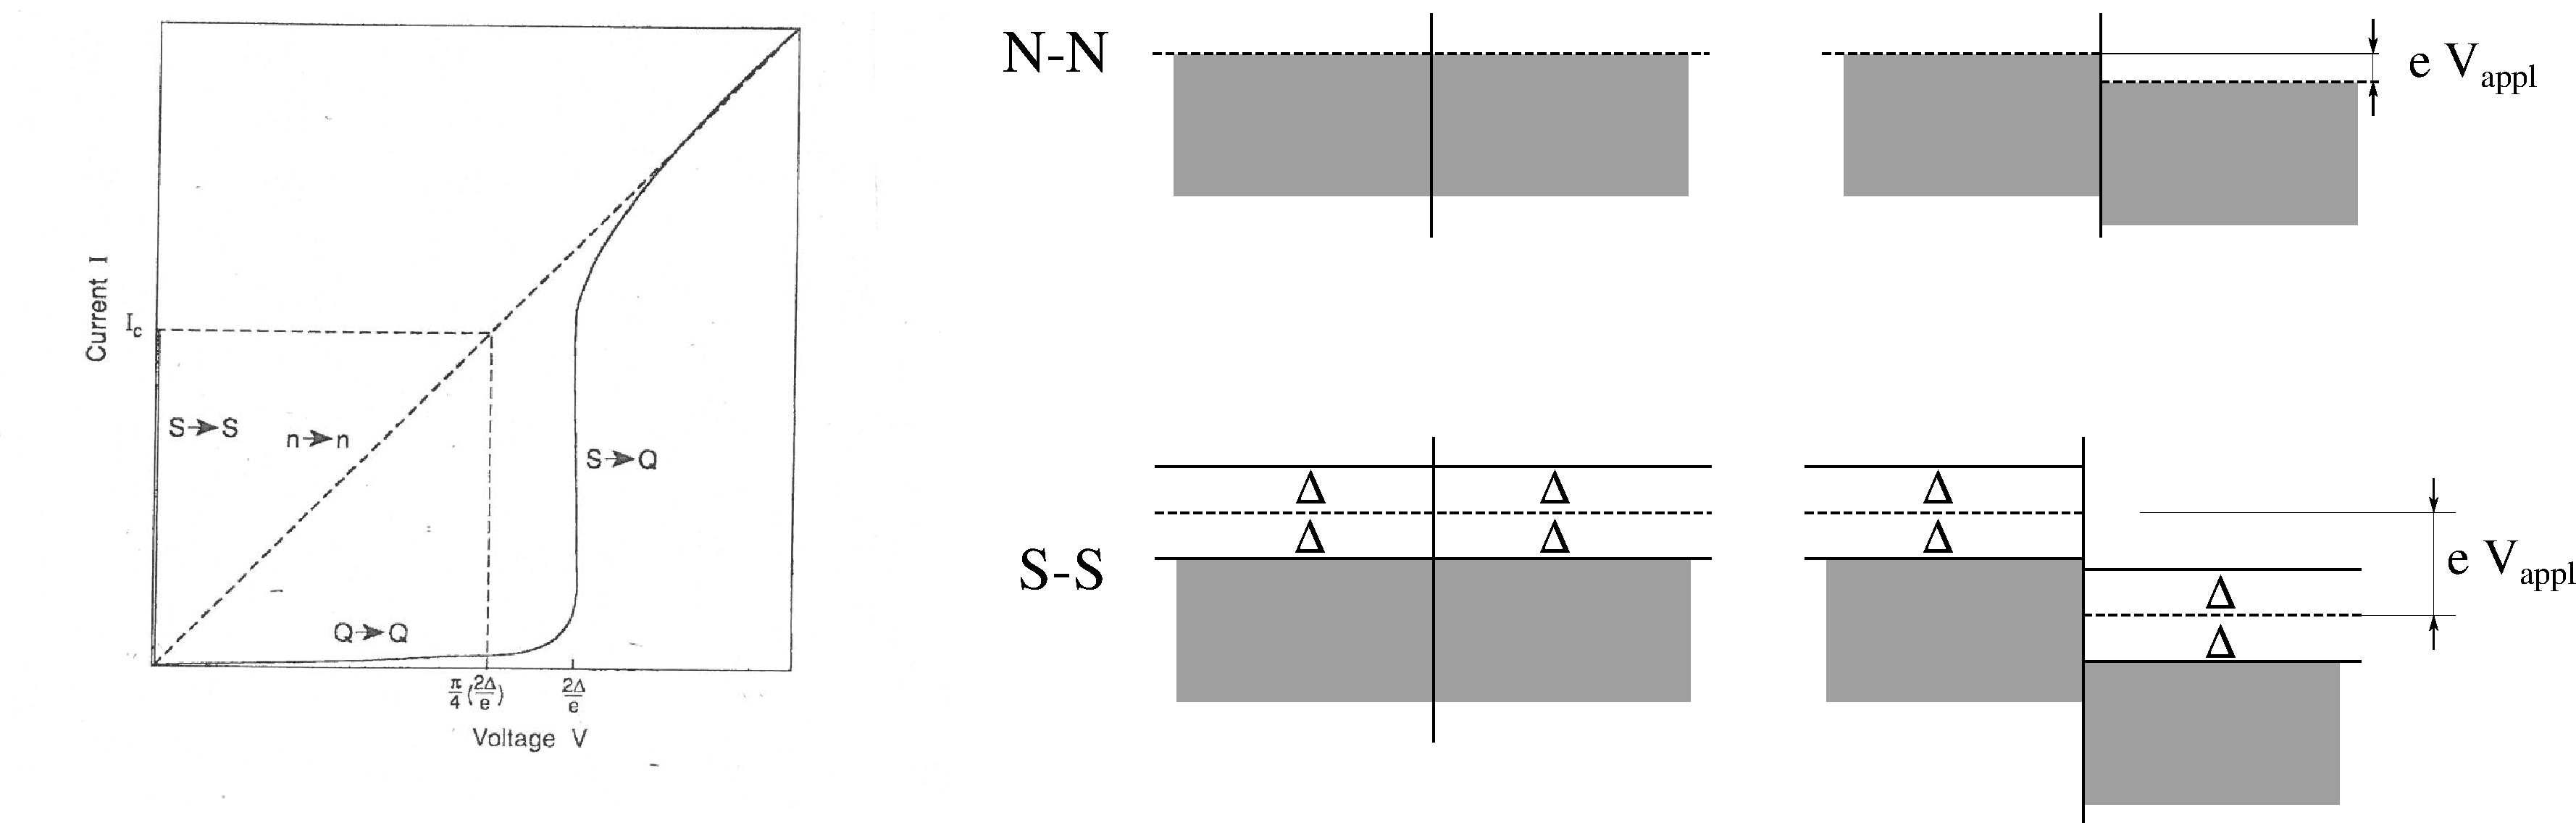
\includegraphics[width=17cm]{C6/figs_C6/fig4_6_1x}}
  	\caption{Current-voltage characteristic curves for tunneling between two metals across a barrier (thin oxide layer of 10--30\AA). It is assumed that both metals are  equal and that they can become superconductors at low temperature (e.g. Al-Al$_2$O$_3$-Al, Sn-SnO$_\text{x}$-Sn). \textbf{N-N} indicates the  current resulting from the \textit{tunneling of single electrons} between the metals, both of them in the normal phase. S-Q indicates the single-electron tunneling between two superconductors \textbf{(S-S)} at finite temperature ($T<T_c$). It shows a small current flow for $0<V<2\Delta/e$, and the usual large flow for $V\gtrsim2\Delta/e$, in which case Cooper pairs are broken and quasiparticles \textbf{(Q)} become excited. \textbf{S-S} labels the (super) current associated with the \textit{tunneling of Cooper pairs} through the unbiased barrier ($V=0$, no potential loss). That is, the (dc) Josephson effect. The critical (dc) Josephson current  is equal to $\pi/4(\approx80\%)$ of the \textbf{N-N} state normal (single electron carrier) current at the gap voltage $V=2\Delta/e$, $2\Delta$ being the energy necessary to break Cooper pairs and excite quasiparticles.}\label{fig4.6.1}
  \end{figure}
  
  For Pb and Sn, the gaps are 1.4 meV and 0.7 meV, leading to $e V_{equiv} \,(V_{equiv})\approx 2.8$ meV (2.8 mV) and 1.4 meV (1.4 mV) respectively. Assuming $R_n$ to be of the order of $1\Omega$ per unit area, implies maximum values of the Josephson supercurrent $J=J_0\sin\gamma$, of the order of $J_0\approx 2$ mA as experimentally observed.
 
 
 It is suggestive that the expression (\ref{eq3.6.19}) is formally similar to that of the ion--ion potential acting between two heavy ions in weak contact, namely at a distance  a diffusivity away from th grazing distance $r_g$. In this case the role of the reduced gap is played by a quantity closely related to the reduced radius of curvature\footnote{\cite{Broglia:04a} p.114  Eq. (40), $U_{aA}^{N}(r)=-V_0/(1+\exp(\frac{r-R_0}{a}))$, $V_0=16\pi\gamma R_{aA}a$, $R_0=R_a+R_A+0.29$ fm, which for two $^{120}$Sn nuclei ($R=5.883$ fm) leads to $R_0\approx12.1$ fm and $V_0=83.8$ MeV. For energies somewhat above the Coulomb barrier, the grazing distance (Eq. (25) p. 128) of the above reference is $r_g=r_B-\delta\approx12.8$ fm ($r_B\approx$ 13.3 fm, $\delta\approx0.5$ fm). Thus $(1+\exp(\frac{r_g+a-R}{a}))\approx10.1$.}
 \begin{align}\label{eq3.6.22}
 U_{aA}^N(r_g+a)\sim \gamma\frac{R_aR_A}{R_a+R_A}a.
 \end{align}
 In the above expression $\gamma\approx$ 0.9 MeV/fm$^2$ is the surface tension, $a=0.63$ fm the diffusivity of the potential, $R_i$(=(1.233$A^{1/3}-0.98A^{-1/3}$) fm) being the radii of nuclei $i=a,A$. For two identical nuclei $R_a=R_A=R$ and $V_0=8\pi\gamma R a$. In the case in which the interacting nuclei are two  $^{120}$Sn systems  $U_{aA}^N(r_g+a)=U_{aA}^N(13.43 \text{ fm})\approx-9$ MeV.
 
 
 
  Nuclei being leptodermous systems can be described at profit, concerning a number of properties, with the help of the liquid drop. Because at the grazing distance the two leptodermous objects overlap, although weakly, two ``unit'' areas disappear. To reconstruct them one has to separate the two nuclei until these areas are reconstructed again. The energy needed to do so has to compensate the value (\ref{eq3.6.22}) which, in the present case  is $\approx$6 MeV. Microscopically, the interaction (\ref{eq3.6.22}) arises from a kind of, weak, covalent mechanism. Single--particle orbitals of the two individual nuclei $a$ and $A$, are shared when in contact, leading to a common mean field.
 
 
 Similarly, the weak limit (\ref{eq3.6.19}) between the two superconductors 1 and 2, is associated with the situations in which each partner of a Cooper pair is in a different superconductor, a kind of incipient covalent phenomenon, each Cooper pair being simultaneously shared by the two superconductors.  
\section{Rotation in gauge space}\label{S3.7}
The occurrence of rotation as a feature of the nuclear spectrum, e.g. of pairing rotational bands, originates in the phenomenon of spontaneous symmetry breaking of rotational invariance in the two dimensional gauge space. In other words, violation of particle number conservation, which introduces a deformation that makes it possible to specify an orientation of the system in gauge space.


The condensate in the nuclear superfluid system involve a deformation of the field that creates the fermion pairs. The process of addition or removal of a Cooper pair constitutes a rotational mode in gauge space in which particle number plays the role of angular momentum. Pairing rotational bands represents the collective mode associated with spontaneous symmetry of particle number conservation.


Let us elaborate on the above points within the framework of a simple model which contains the basic physical features one is interested in discussing.


We consider $N$ nucleons moving in a single $j$--shell\footnote{For details see e.g. App. H of \cite{Brink:05} and refs. therein.} of energy $\epsilon_j$ and total angular momentum $(ls)j$. The number of pairs moving in time reversal state which can be accommodated in the shell is $\Omega=(2j+1)/2$. Consequently, the value of the BCS occupation parameters is $V=(N/2\Omega)^{1/2}$ and $U=(1-N/2\Omega)^{1/2}$. Setting $\epsilon_j=0$. The solution of the BCS number and gap equations associated with a pairing force with constant matrix elements $G$ are
  \begin{align}\label{eq3.7.1}
  \lambda=-\frac{G}{2}(\Omega-N),
  \end{align}
  and
  \begin{align}\label{eq3.7.2}
\Delta=\frac{G}{2}\sqrt{N(2\Omega-N)},
  \end{align}
respectively.


The BCS ground state energy of the superfluid system is
  \begin{align}\label{eq3.7.3}
U=2\sum_{\nu>0}(\epsilon_\nu-\lambda)V^2_\nu-\frac{\Delta^2}{G}.
  \end{align}
Using (\ref{eq3.7.1}) and (\ref{eq3.7.2}), one can write
  \begin{align}\label{eq3.7.4}
U\approx\frac{\hbar^2}{2\mathcal J}N^2,  
    \end{align}
where
  \begin{align}\label{eq3.7.5}
\mathcal J=\frac{2\hbar^2}{G},  
    \end{align}
is the moment of inertia of the associated pairing rotational band. The fact that the single--particle energies are measured with respect to $\lambda$ implies that the nucleons feel the Coriolis force ($\hbar\dot{\phi}=\lambda$) associated with rotation in gauge space (Eq. (\ref{eq3.7.11}) below). In other words, the BCS solution is carried out in the intrinsic system of reference $\mathcal K'$ (see below). In fact, the ground state energy in the laboratory system $\mathcal K$ is (see Fig. \ref{fig1.3}\footnote{\cite{Broglia:00}.})
  \begin{align}\label{eq3.7.6}
E_0=U+\lambda N=\lambda N+\frac{\hbar^2}{2\mathcal J}N^2.
    \end{align}















\subsection{Phase coherence}\label{C3AppD}
The phase of a wavefunction and the number of nucleons (electrons in condensed matter) are conjugate variables. In other words, the gauge angle and the particle number operators $\hat{\phi}$ and $\hat N$ satisfy the commutation relation,
  \begin{align}\label{eq3.7.8}
\left[\hat{\phi},\hat{N}\right]=i.
    \end{align}
In the particle number representation
  \begin{align}\label{eq3.7.9}
\hat N=-i\partial/\partial \phi,\quad \hat \phi=\phi,
    \end{align}
while
  \begin{align}\label{eq3.7.10}
\hat N=N,\quad \hat\phi=i\partial/\partial N,
    \end{align}
in the gauge angle representation. The time derivative of the gauge angle is given by the equation of motion\footnote{See e.g. \cite{Brink:05} App. I.},
  \begin{align}\label{eq3.7.11}
  \dot{\phi}=\frac{i}{\hbar}\left[H,\phi \right]=\frac{1}{\hbar}\frac{\partial H}{\partial N}=\frac{1}{\hbar}\lambda,
    \end{align}
where $\lambda$ is the chemical potential (Fermi energy).







 Gauge invariance, i.e. invariance under phase changes, implies number of particle conservation in a similar way that rotational invariance implies angular momentum conservation.

Example: let us introduce the trivially invariant many-body wavefunction\footnote{\cite{Anderson:64b}.},
\begin{align}\label{eq3.7.12}
\Psi=a_1^\dagger a_2^\dagger\dotsb a_N^\dagger \Psi_{vac},
\end{align}
and rotate it an angle $\phi$ making use of the operator
\begin{align}\label{eq3.7.13}
\mathcal G(\phi)\ket{\Psi_N}=e^{-iN\phi}\ket{\Psi}=\ket{\Psi'},
\end{align}
where
\begin{align}\label{eq3.7.14}
\ket{\Psi'}=a_1'^\dagger a_2'^\dagger\dotsb a_N'^\dagger\ket{0},
\end{align}
and
\begin{align}\label{eq3.7.15}
\mathcal G^{-1}(\phi)a_\nu^\dagger \mathcal G(\phi)=e^{-i\phi}a_\nu^\dagger=a_\nu'^\dagger,
\end{align}
thus
\begin{align}\label{eq3.7.16}
\ket{\Psi_N}=e^{iN\phi}\ket{\Psi'_N},
\end{align}
and
\begin{align}\label{eq3.7.17}
\hat N\ket{\Psi_N}=-i\frac{\partial}{\partial \phi}\ket{\Psi_N}=N\ket{\Psi_N}.
\end{align}
 A phase change for a gauge invariant function is just a trivial operation. Like to rotate a rotational invariant function. Quantum mechanically nothing happens rotating a spherical, symmetry conserving, system (in 3D-, gauge, etc.) space.


The situation is very different in the case of the wavefunction
\begin{align}\label{eq3.7.7}
\nonumber|BCS(\phi)\rangle_{\mathcal{K}} &=\prod_{\nu>0}\left(U_\nu+V_\nu a_\nu^\dagger a_{\bar \nu}^{\dagger}\right)|0\rangle,\\
\nonumber&=\prod_{\nu>0}\left(U'_\nu+e^{-2i\phi}V'_\nu a^\dagger_\nu a^{\dagger}_{\bar \nu}\right)|0\rangle,\\
\nonumber&=\prod_{\nu>0}\left(U'_\nu+V'_\nu a'^\dagger_\nu a'^{\dagger}_{\bar \nu}\right)|0\rangle,\\
&=|BCS(\phi=0)\rangle_{\mathcal{K'}},
\end{align}
where 
\begin{align}
U_\nu=|U_\nu|=U'_\nu;\quad V_\nu=e^{-2i\phi}V'_\nu \;(V'_\nu=|V_\nu|).
\end{align}
In fact,
\begin{align}\label{eq3.7.19}
|BCS(\phi)\rangle_{\mathcal{K}}=\left(\prod_{\nu>0}U_\nu'\right)\sum_{N\text{ even}}\frac{e^{-iN\phi}}{(N/2)!}\left(\sum_{\nu>0}c'_\nu P^\dagger_\nu\right)^{N/2}|0\rangle,
\end{align}
with
\begin{align}
c_\nu'=\frac{V_\nu'}{U_\nu'};\quad \quad P^\dagger_\nu=a^\dagger_\nu a^\dagger_{\bar\nu},
\end{align}
is a coherent state in particle number which can be written as,
\begin{align}\label{eq3.7.21}
\ket{BCS(\phi)}_{\mathcal K}=\sum_N f_N(\phi)\ket{\Psi_N}
\end{align}
Let us now apply the gauge angle operator to it,
\begin{align}
\hat{\phi}\ket{BCS(\phi)}_{\mathcal K}=\hat{\phi}\sum_{N}f_N(\phi)\ket{\Psi_N},
\end{align}
that is,
\begin{align}
i\frac{\partial}{\partial N}f_N(\phi)=\phi f_N(\phi).
\end{align}
Thus,
\begin{align}
f_N(\phi)\sim e^{-iN\phi},
\end{align}
and
\begin{align}
\ket{BCS(\phi)}_{\mathcal K}\sim \sum_{N} e^{-iN\phi}\ket{\Psi_N},
\end{align}
 the state $|BCS(\phi=0)\rangle_{\mathcal{K}'}$ being aligned in gauge space in which it defines a privileged orientation ($z'$).


An isolated nucleus will not remain long in this product type state. Due to the term\footnote{Within BCS theory of pairing, there are two parameters which determines spontaneous symmetry breaking in gauge space. The probability amplitude with which a pair state ($\nu\bar{\nu}$) is occupied, and that with which it is empty. Namely, $V_\nu$ and $U_\nu$ respectively. As a consequence, there only two fields $F$ which contribute, through terms of type $FF^\dagger$, to the residual interaction $H_{res}$ acting among quasiparticles, which is neglected in the mean field solution of the pairing Hamiltonian. One which is antisymmetric with respect to the Fermi surface namely ($U^2_\nu-V^2_\nu)$ and which leads to pairing vibrations of the gauge deformed state $\ket{BCS}$. The other one, ($U^2_\nu+V^2_\nu)$ is symmetric with respect to $\epsilon_F$ and leads to fluctuations which diverge in the long wavelength limit ($W''_1\to0$) in precisely the right way to set $\ket{BCS}$ into rotation with a finite inertia, and restore symmetry (see Eq. \ref{eq0.1.92}).}  $(G/4)\left(\sum_{\nu>0}\left(U^2_\nu+V^2_\nu\right)\left(\Gamma_\nu^\dagger-\Gamma_\nu\right)\right)^2$ in the residual quasiparticle Hamiltonian it will fluctuate, and decay into a state
\begin{align}\label{eqbeta}
|N\rangle \sim \int d\phi e^{iN\phi}|BCS(\phi)\rangle_{\mathcal{K}}\sim \sum_{N'}\int_0^{2\pi}d\phi\, e^{-i(N'-N)\phi}\ket{\Psi_{N'}}\sim\ket{\Psi_{N}}
\end{align}
in keeping with the fact that
\begin{align}\label{eq3.7.27}
\int_0^{2\pi}d\phi\, e^{-i(N'-N)\phi}=\left\{
\begin{array}{c}
 2\pi\delta(N,N')\quad (N=N'),\\ 
 \\
\left.\frac{i}{N'-N}e^{-i(N'-N)\phi}\right|^{2\pi}_0=0\quad (N\neq N').
\end{array} \right.
\end{align}
The state $\ket{N}$ is a member of the pairing rotational band centered around neutron number $N_0$. In the example discussed in connection with Figs. \ref{fig1.2} and \ref{fig1.3}, $\ket{N}$ is one of the ground states of the Sn-isotopes around $N_0=68$. Making use of the fact that $E_R=\left(\hbar^2/2\mathcal I\right)(N-N_0)^2$ and that $\delta N\delta\phi\approx1$, the coherent state (\ref{eq3.7.21}) will decay into one of the states $\ket{N}$, likely the one corresponding to $N=\sum_{\nu>0}2V_\nu^2$, in a time $\hbar/E_R$. The member of  Cooper pairs participating in the nuclear condensate in the case of $^{120}$Sn is $\alpha'_0\approx5-6$, the number of neutrons being $2\alpha'_0\approx10$. Because $\delta N\sim\sqrt{N}\sim3$ ($\delta\phi\sim0.3$ rad, that is\footnote{$\delta\phi\approx0.3/(\pi/180)\approx0.3/0.017\approx17^\circ$.} $\delta\phi\sim0.3/0.017\approx 17^\circ$), the energy of rotation in gauge space of a state which is defined with an uncertainty of $\delta\psi\approx0.3$ rad is  $E_R\approx0.092$ MeV$\times(3)^2\approx 1$ MeV ($\hbar^2/2\mathcal I\approx G/4\approx 25\text{ MeV}/(4N_0)\approx0.092$ MeV, see Fig. \ref{fig1.3}). Consequently $\hbar/E_R\approx10^{-21}$s. 


This is also the case for metallic superconductors. In fact, the state (\ref{eq3.7.7}) even if prepared in isolation will dissipate because there is a term in the energy of the superconductor depending on $N$, namely the electrostatic energy $e^2(N-N_0)^2/2C$, where $C$ is the electrostatic capacity\footnote{The capacity of a sphere is $C=R$. Below we use $R=1$cm (see \cite{Anderson:64b}).}. Because the number of overlapping Cooper pairs contributing to superconductivity is $\alpha'_0\approx10^6$ and thus the associated number of electrons $2\alpha'_0\approx2\times10^6$, $\delta N\sim\sqrt{N}\sim10^3$, one can write $E_{el}=\frac{e^2}{2C}(\delta N)^2\approx\frac{14.4\text{ eV}\times10^{-8}\text{ cm}}{2\times1\text{ cm}}(10)^3\approx10^{-7}$ eV, and $\hbar/E_{el}\approx 10^{-14}$ s.  In this case $\delta\phi\sim10^{-3}$ radians, that is $\delta\phi\sim10^{-3}/0.017\sim1^{\circ}$.   
The opposite situation is that of the case in which one considers different parts of the same superconductor. In this case one can define relative variables $n=N_1-N_2$ and $\phi=\phi_1-\phi_2$ and again $n=-i\partial/\partial \phi$ and $\phi=i\partial/\partial n$. Thus, locally there is a superposition of different $n$ states: $\phi$ is fixed so $n$ is uncertain.There is  a dividing line between these two behaviors, perfect phase coherence and negligible coherence, namely the Josephson effect.


Again, the total phase of the assembly is not physical. However, the relative phases can be given a meaning when one observes, as one does in e.g. metallic superconductors, that electrons can pass back and forth through the barrier, leading to the possibility of coherence between states in which the total number of electrons is not fixed \emph{locally}. Under such conditions there is, for instance, a coherence between the state with $N/2$ electrons in one half of the block and $N/2$ in the other, and that with $(N/2)+2$ on one side side and $(N/2)-2$ on the other.









%\begin{figure}\centerline{\includegraphics*[width=10cm,angle=0]{nutshell/figs/fig3D1.pdf}}
%\caption{Gedanken experiment concerning the possibility of observing weak coupling coherence phenomena between states $|BCS(A+2)\rangle$ and $|BCS(A)\rangle$ in an elastic reaction involving superfluid nuclei (\textbf{a}), e.g. $p+^{120}$Sn$\rightarrow p+^{120}$Sn, the system $^{119}$Sn+$d$ acting as a dynamical barrier (hatched areas arguably play role of that of dioxide layers in Josephson junctions) between the two even $N$ superfluid systems arising from the successive transfer of two nucleons (\textbf{b}) and eventually allowing for  a time dependent gauge phase difference between the $(A+2)$ and $A$ superfluid systems, thus leading, in the case in which $Q$--value effects are appropriate, to an oscillating enhancement of the elastic cross section at large angles as observed, for quite different reasons, in the case of the elastic angular distribution of the reaction $^{16}$O+$^{28}$Si (\textbf{c}) (cf. \cite{Pollarolo:84}).}\label{fig3.C.1}
%\end{figure}

\section{Hindsight}\label{C3AppE}
The formulation of superconductivity (BCS theory) described by Gor'kov\footnote{\cite{Gorkov:58,Gorkov:59}.} allows, among other things for a simple visualization of spatial dependences. In this formulation $F(\mathbf{x},\mathbf{x}')$ is the amplitude for two Fermions (electrons) at $\mathbf{x},\mathbf{x}'$, to belong to the Cooper pair (within the framework of nuclear physics cf. e.g. Fig. \ref{fig1F3} $\Psi_0(\mathbf{r}_1,\mathbf{r}_2)$; see also App. \ref{App3B}). The phase of $F$ is closely  related to the angular orientation of the spin variable  in Anderson's quasispin formulation of BCS theory\footnote{\cite{Anderson:58b}; within the framework of nuclear physics cf. e.g. \cite{Bohr:88}, \cite{Potel:13b} and references therein.}. The gap function $\Delta(x)$ is given by $V(\mathbf{x})F(\mathbf{x},\mathbf{x})$ where $V(\mathbf{x})$ is the local two--body interaction at the point $\mathbf x$. In the insulating barrier between the two superconductors of a Josephson junction, $V(\mathbf{x})$ is zero and thus $\Delta(x)$ is also zero. 



The crucial point is that vanishing\footnote{This point was likely misunderstood by Bardeen who writes``\dots In my view, virtual pair excitations do not extend across the layer\dots'', see \cite{McDonald:01}, see also \cite{Bardeen:61} and \cite{Bardeen:62}.} $\Delta(x)$ does not imply vanishing $F$, provided, of course, that one has within the insulating barrier, a non-zero particle (electron) density, resulting from the overlap of densities from right (R) and left (L) superconductors. Now, these barriers are such that they allow for one-electron-tunneling with a probability of the order of 10$^{-10}$ and, consequently, the above requirement is fulfilled. Nonetheless, conventional (normal) simultaneous pair transfer, with a probability of $(10^{-10})^2$ will not be observed\footnote{\cite{Pippard:12} see also \cite{McDonald:01}.}. \textit{But because one electron at a time can tunnel profiting of the small, but finite electron density within the layer,   $F(\mathbf{x},\mathbf{x}')$ can have a sizable amplitude for Cooper pairs with partners electrons one on each side of the barrier (i.e. $\mathbf x\in$ L and $\mathbf x'\in$ R), separated by distances $|\mathbf{x}-\mathbf{x}'|$ up to the coherence length}. Hence, for barriers thick to only allow for essentially the tunneling of one electron at a time, but thin compared with the coherence length, two electrons on opposite sides of the barrier can still be correlated and the pair current   be consistent. An evaluation of its 
value shows that, at zero temperature, the pair current is equal to $\pi/4$ times the normal, single electron carrier current, at an equivalent voltage\footnote{In the case of Pb at low temperatures ($\approx7.19$ K (0.62 meV)) this voltage is $\approx 1$ meV/$e=1$ mV leading to $\approx$2mA current for a barrier resistance of $R\sim1\Omega$ (\cite{Ambegaokar:63,McDonald:01,Tinkham:96}).} $2\Delta/e$.


The translation of the above parlance to the language of nuclear physics has to come to terms with the basic fact that nuclei are self--bound, finite many--body systems in which the surface, as well as space quantization, play a very important role both as a static element of confinement, as well as a dynamic source for renormalization effects\footnote{Within this context it is of notice that the liquid drop model is a very successful nuclear model, able to accurately describe not only large amplitude motion (fission, exotic decay, low-lying collective density and surface vibrations, cf. e.g. \cite{Bohr:39}, \cite{Bertsch:88b}, \cite{Barranco:90}, and references therein), but also the masses of nuclides (see e.g. \cite{Moller:95}), provided the superfluid inertia and shell corrections respectively, are properly considered. Thus, it is likely that in the quest of  more predictive theoretical tools of the global nuclear properties one should develop on equal footing ever more ``accurate'' bare $NN$-potentials as well as effective forces, and methods to deal with the long wavelength, renormalization effects and induced interactions. Within this context it is illuminating the contribution of \cite{Anderson:62} concerning the nuclear surface diffuseness, at the time of the development of  Brueckner theory (\cite{Brueckner:61}).}$^,$\footnote{\cite{Broglia:02d}.}.
Under the influence of the average potential which can be viewed as very strong external field $(|V_0|\approx 50$ MeV), Cooper pairs ($|E_{corr}|\approx 1.2$ MeV; see e.g. Fig. \ref{fig1E1}) will become constrained within its boundaries with some amount of spill out. In the case of the single open shell superfluid nucleus $^{120}$Sn, the boundary can be characterized by the radius $R_0\approx 6$ fm ($\ll \xi\approx 14$ fm), the spill out being connected with the diffusivity $a\approx 0.65$ fm. 


Let us now consider a two nucleon transfer reaction in the collision Sn+Sn assuming a distance of closest approach of $\approx 14$ fm, in which the two nuclear surfaces are separated by $\approx 2$ fm (Fig \ref{fig_1}). In keeping with the fact that this distance is about 3$\times a$, the heavy ion system will display a few percent (of saturation) density overlap in the interacting region. Ever so small this overlap of the nuclear surfaces, and so narrow the hole between the two leptodermic systems resulting from  it,  Cooper pairs can now extend over the two volumes, in a similar way as electron Cooper pairs could be partially found in the R and L superconductors in a Josephson junction. If this is the case, Cooper pair partners can, in principle, be at distance as large as 26 fm, of the same order of magnitude as twice the correlation length (see Sects. \ref{App4.B.3} and \ref{S7.3}). 

  As previously stated, an example of the fact that Cooper pairs will ``expand'' if the external mean field allows for it, is provided by $^{11}$Li in which case, profiting of the weak binding ($\approx 380$ keV), the extension of the constrained Cooper  pair ($\approx 4.58 $ fm $\pm 0.13$ fm)   is similar to that expected in a nucleus of mass number $A\approx 60$, assuming a standard radial behavior, i.e. $r_0 A^{1/3}$ fm. In keeping with this scenario, it could be expected that moving from one neutron pair addition $0^+$ mode of the $N=6$ isotones\footnote{See e.g. \cite{Gori:04}.} to another one ($|^{11}\text{Li(gs)}\rangle$, $|^{12}\text{Be(gs)}\rangle$ and $|^{12}\text{Be}(0^{+*};2.24\,\text{MeV})\rangle$) one would see the system expanding, contracting and expanding again, respectively, in keeping with the fact that the external (mean) field is weak, strong, weak respectively, as testified by $S_{2n}$ (380 keV, 3672 keV, 1432 keV).  
Within this context, in Fig. \ref{fig3.8.1} an overall view of the pairing vibrational modes associated with $N=6$ parity inverted closed shell isotones, together with low-energy $E1$-strength modes is given. The possible candidates to the role of neutron halo pair addition modes and symbiotic state are explicitly indicated (boxed levels).
   \begin{figure}
   	\centerline{\includegraphics*[width=21cm,angle=90]{nutshell/figs/fig3_8_1_v3}}
   	\caption{Monopole pairing vibrational modes associated with 
   		$N=6$ parity inverted closed shell isotones, together with low-energy E1-strength modes. 
   		The levels are  displayed as a function of the two-neutron separation energies $S(2n)$. 
   		These quantities are shown in parenthesis, the excitation energies with respect to the ground state are quoted in MeV. 
   		Absolute differential cross sections from selected $(t,p)$ and $(p,t)$ reactions calculated as described in the text (cf. \cite{Potel:10,Potel:14}), 
   		in comparison with the experimental data (\cite{Young:71,Fortune:94}).}\label{fig3.8.1}
   \end{figure}
%   \begin{figure}
%   	\centerline{\includegraphics*[width=\textwidth,angle=0.]{nutshell/figs/fig3_8_2x}}
%   	\caption{}\label{fig3.8.2}
%   \end{figure}





\begin{subappendices}
\section{Medium polarization effects and pairing}\label{C3AppEx}
In many-body systems, medium polarization effects play an important role in renormalizing single-particle motion and the four-point vertices, namely Coulomb interaction in condensed matter and the bare $NN$-potential in nuclei. In what follows, special attention is paid to this mechanism in connection with the pairing interaction.
\subsection{Nuclei}\label{S4.A.1}
Elementary modes of excitation constitute a basis of states in which correlations, as found in observables, play an important role. As a consequence, it allows for an economic solution of the nuclear many--body problem of structure and reaction.


Also as a result of their interweaving,  the variety of elementary modes of excitation may break in a number of states, eventually acquiring a lifetime and, within a coarse grain approximation, a damping width (imaginary component of the self energy). Moving into the continuum, as for example in the case of direct reactions, one such component is the imaginary part of the optical potential operating in the particular channel selected. It can, in principle, be calculated microscopically using similar techniques and elements as e.g. those used in the calculation of the damping width of giant resonances or of single-particle motion. In this way, the consistency circle structure-reaction based on elementary modes and codified by NFT could be closed. The rich variety of emergent properties found along the way eventually acquiring a conspicuous level of physical validation. At that time it would be possible, arguably if there is one, to posit that the \textit{ultima ratio} of structure and reactions, in any case that associated with pairing and Cooper pair transfer in nuclei, have been unveiled\footnote{In the above paragraph we allowed ourselves to paraphrase Jacques Monod writing in connection with biology and life: L'\textit{ultima ratio} de toutes les structures et performances t\'el\'eonomiques des \^etres vivants est donc enferm\'ee dans les s\'equences des radicaux des fibres polypeptidiques ``embryons'' de ces d\'emons de Maxwell biologiques que sont les prot\'eines globulaires. En un sens, tr\`{e}s r\'{e}el, c'est \`a ce niveau d'organisation chimique qui g\^it, s'il y en a un, le secret de la vie. Et saurait--on non seullement d\'ecrire les s\'equences, mais \'enoncer la loi d'assemblage \`a laquelle ob\'eissent, on pourrait dire que le secret est perc\'e, l'ultima ratio d\'ecouverte (\cite{Monod:70}).}
\subsubsection{Effective moments}
At the basis of the coupling between elementary modes of excitation, for example of single--particle motion and of collective vibrations, one finds the fact that, in describing the nuclear structure it is necessary to make reference to both of them simultaneously and in an unified way.
   \begin{figure}
   \centerline{\includegraphics*[width=8cm,angle=0	]{nutshell/figs/fig3_A_1}}
   \caption{(a) $F$-moment of single-particle and (b,c) renormalization effects induced by the collective vibration $\alpha$.}\label{fig3.A.1}
   \end{figure}

Within the harmonic approximation the above statement is economically embodied in e.g. the relation existing between the collective $(\hat \alpha)$ and the single--particle $(\hat F)$ representation of the operator creating a particle--hole excitation. That is\footnote{cf. \cite{Bohr:75}, cf. also \cite{Brink:05} App. C.}, 
\begin{align}\label{eq1AppE1}
\nonumber \hat F&=\left\{\braket{k|F|\tilde i}\Gamma_{ki}^\dagger+\braket{\tilde i|F|k}\Gamma_{ki}\right\}\\
\nonumber &=\sum_{k,i,\alpha'}X_{ki}^{\alpha'}\Gamma_{\alpha'}^{\dagger}-Y_{ki}^{\alpha'}\Gamma_{\alpha'}\\
\nonumber &=\sum_{\alpha'}\Lambda_{\alpha'}\sum_{ki}\frac{\left|\braket{\tilde i|F|k}\right|^22(\epsilon_i-\epsilon_k)}{(\epsilon_k-\epsilon_i)^2-(\hbar\omega_{\alpha'})^2}\left(\Gamma_{\alpha'}^\dagger+\Gamma_{\alpha'}\right)\\
 &=\sum_{\alpha'}\frac{\Lambda_{\alpha'}}{\kappa}\left(\Gamma_{\alpha'}^{\dagger}+\Gamma_{\alpha'}\right)=\sum_{\alpha'}\sqrt{\frac{\hbar\omega_{\alpha'}}{2C_\alpha'}}\left(\Gamma_{\alpha'}^{\dagger}+\Gamma_{\alpha'}\right)=\hat \alpha.
\end{align}
This is a consequence of the self consistent relation
\begin{align}
\delta U(r)=\int d\mathbf r' \delta \rho(r)v(|\mathbf r{-\mathbf r'}|),
\end{align}
existing between density (collective) and potential (single--particle) distortion, typical of normal modes of many--body systems.

Relation (\ref{eq1AppE1}) implies that at the basis of these normal modes one finds the (attractive $\kappa<0$) separable interaction 
\begin{align}\label{eq3AppE1}
H=\frac{\kappa}{2}\hat F\hat F,
\end{align}
but where now (Fig. \ref{fig3.A.1} (a))
\begin{align}
\hat F=\sum_{\nu_1,\nu_2} \braket{\nu_1|F|\nu_2}a^\dagger_{\nu_1}a_{\nu_2},
\end{align}
is a general single--particle operator, while $\hat F$ in  Eq. (\ref{eq1AppE1}) is its harmonic representation acting in the particle $(k)$--hole ($i$) space, $\Gamma^\dagger_{ki}$ and $\Gamma_{ki}$ being (quasi) bosons, i.e. respecting the commutation relation 
\begin{align}
\left[\Gamma_{ki},\Gamma^\dagger_{k'i'}\right]=\delta(k,k')\delta(i,i').
\end{align}
In other words, the representation (\ref{eq1AppE1}), which is at the basis of the RPA (as well as QRPA), does not allow for scattering vertices, processes which become operative by rewriting (\ref{eq3AppE1}) in terms of the particle--vibration coupling Hamiltonian
\begin{align}\label{eq3AppE4}
H_c=\kappa\hat \alpha\hat F
\end{align}
\emph{It is of notice that $\kappa$ is negative for an attractive field}. Let us now calculate the effective single--particle moments (cf. Fig. \ref{fig3.A.1} (b)),
\begin{align}
\nonumber \braket{\nu_2|\hat F|\nu_1}_{(b)}=&\frac{\braket{\nu_2|\hat F|\nu_2,n_\alpha=1}\braket{\nu_2,n_\alpha=1|H_c|\nu_1}}{(\epsilon_{\nu_1}-\epsilon_{\nu_2})-\hbar\omega_\alpha},\\
\nonumber &=\frac{\braket{0|\hat \alpha|n_\alpha=1}\kappa\alpha \braket{\nu_2|F|\nu_1}}{(\epsilon_{\nu_1}-\epsilon_{\nu_2})-\hbar\omega_\alpha},\\
&=\kappa\alpha^2\frac{ \braket{\nu_2|F|\nu_1}}{(\epsilon_{\nu_1}-\epsilon_{\nu_2})-\hbar\omega_\alpha},
\end{align}
and (Fig. \ref{fig3.A.1} (c))\footnote{In calculating the energy denominators one takes the difference between the energy of the initial and of the intermediate states. However, when an external field like $\hat F$ acts on the system, before the PVC or four-point vertices operate, being equivalent to an observation, the energy denominator is to be calculated as the energy difference between the final and the intermediate states. }
\begin{align}\label{eq8App1E}
\nonumber \braket{\nu_2|\hat F|\nu_1}_{(c)}&=\frac{\braket{\nu_2|H_c|\nu_1,n_\alpha=1}\braket{\nu_1,n_\alpha=1| F|\nu_1}}{\epsilon_{\nu_2}-(\epsilon_{\nu_1}+\hbar\omega_\alpha)},\\
&=\kappa\alpha^2\left(-\frac{\braket{\nu_2|F|\nu_1}}{(\epsilon_{\nu_1}-\epsilon_{\nu_2})+\hbar\omega_\alpha}\right),
\end{align}
leading to 
\begin{align}
\nonumber \braket{\nu_2|\hat F|\nu_1}_{(b)}&+\braket{\nu_2|\hat F|\nu_1}_{(c)}=\kappa\alpha^2\frac{2\hbar \omega_\alpha\braket{\nu_2|F|\nu_1}}{(\epsilon_{\nu_1}-\epsilon_{\nu_2})^2-(\hbar\omega_\alpha)^2},\\
&=\frac{\kappa}{C_\alpha}\frac{(\hbar\omega_\alpha)^2\braket{\nu_2|F|\nu_1}}{(\epsilon_{\nu_1}-\epsilon_{\nu_2})^2-(\hbar\omega_\alpha)^2}.
\end{align}
This is in keeping with the fact that the ZPF of the $\alpha$-vibrational mode is,
\begin{align}
\alpha=\sqrt{\frac{\hbar\omega_\alpha}{2C_\alpha}}.
\end{align}
The particle-vibration coupling strength used below is defined as,
\begin{align}
\Lambda_\alpha=\kappa\alpha.
\end{align}
Together with $\braket{\nu_2|\hat F|\nu_1}_{(a)}=\braket{\nu_2|F|\nu_1}$ (see Fig. \ref{fig3.A.1} (a)) one obtains
\begin{align}\label{eq3.A.12}
\braket{\nu_2|\hat F|\nu_1}=\left(1+\chi(\omega)\right)\braket{\nu_2|F|\nu_1},
\end{align}
where
\begin{align}\label{eq3.A.13}
 \chi_\alpha(\omega)=\frac{\kappa}{C_\alpha}\frac{\omega_\alpha^2}{\omega^2-\omega_\alpha^2}
\end{align}
is the polarizability coefficient while
\begin{align}\label{eq3.A.14}
\omega=|\epsilon_{\nu_1}-\epsilon_{\nu_2}|/\hbar.
\end{align}
In the static limit, e.g. in the case in which $\alpha$ is a giant resonance and $\omega_\alpha\gg\omega$ one obtains
\begin{align}\label{eq3.A.15}
\chi_\alpha(0)=-\frac{\kappa}{C_\alpha}.
\end{align}
The sign of $\chi_\alpha(0)$ is opposite to that of $\kappa$, since the static polarization effect produced by an attractive coupling ($\kappa<0$) is in phase with the single--particle moment, while a repulsive coupling ($\kappa>0$) implies opposite phases for the polarization effect and the one--particle moment\footnote{\cite{Bohr:75,Mottelson:62}. Think in the first case about the effect the GQR ($\tau=0$) plays in $(e(E2))_{eff}$, in the second that played by the GDR ($\tau=1$) in $(e(E1))_{eff}$.}.



Let us now calculate the two-body pairing induced interaction (Fig. \ref{fig3.A.2}) arising from the exchange of collective vibrations\footnote{In the present discussion we do not consider spin modes. For details see e.g. \cite{Idini:15}. See also \cite{Bortignon:83}.},  summing over the two time orderings and symmetrizing between initial and final states\footnote{Cf. \cite{Brink:05} p. 217.}
\begin{align}
\nonumber v_{\nu\nu'}^{ind}(a)+v_{\nu\nu'}^{ind}(b)&=\kappa^2\alpha^2\left|\braket{\nu'|F|\nu}\right|^2\left(\frac{1}{\epsilon_\nu-\epsilon_{\nu'}-\hbar\omega_\alpha}+\frac{1}{\epsilon_{\nu'}-\epsilon_{\nu}-\hbar\omega_\alpha}\right),\\
\nonumber &=\kappa^2\alpha^2\left|\braket{\nu'|F|\nu}\right|^2\left(\frac{1}{(\epsilon_\nu-\epsilon_{\nu'})-\hbar\omega_\alpha}-\frac{1}{(\epsilon_{\nu}-\epsilon_{\nu'})+\hbar\omega_\alpha}\right),\\
\nonumber &=\Lambda_\alpha^2\left|\braket{\nu'|F|\nu}\right|^2\left(\frac{2\hbar\omega_\alpha}{(\epsilon_\nu-\epsilon_{\nu'})^2-(\hbar\omega_\alpha)^2}\right),\\
&=v_{\nu\nu'}^{ind}(c)+v_{\nu\nu'}^{ind}(d).
\end{align}
   \begin{figure}
   \centerline{\includegraphics*[width=12cm,angle=0	]{nutshell/figs/fig3_A_2}}
   \caption{Diagrams associated with nuclear pairing induced interaction.}\label{fig3.A.2}
   \end{figure}
Thus
\begin{align}\label{eq3.A.17}
\nonumber v_{\nu\nu'}^{ind}&=\frac{1}{2}\left(v_{\nu\nu'}^{ind}(a)+v_{\nu\nu'}^{ind}(b)\right)+\frac{1}{2}\left(v_{\nu\nu'}^{ind}(c)+v_{\nu\nu'}^{ind}(d)\right)\\ &=\Lambda_\alpha^2\left|\braket{\nu'|F|\nu}\right|^2\left(\frac{2\hbar\omega_\alpha}{(\hbar\omega)^2-(\hbar\omega_\alpha)^2}\right).
\end{align}
The diagonal matrix element,
\begin{align}
\nonumber v_{\nu\nu}^{ind}\equiv-\frac{2\Lambda_\alpha^2\left|\braket{\nu|F|\nu}\right|^2}{\hbar\omega_\alpha},
\end{align}
testifies to the fact, for values of $\omega_\alpha\gtrsim\omega$, 
 the induced pairing interaction is attractive.
Summing to (\ref{eq3.A.17}) the matrix element of the bare interaction (\ref{eq3AppE1}), (Fig. \ref{fig3_A_3} (b))\footnote{Within the framework of (\ref{eq3AppE1}) and of its role in (\ref{eq17App1E}) one finds, in the case of superconductivity in metals to be discussed below,  that the bare unscreened Coulomb interaction can be written as 
	\begin{align*}
	U_c(r)=\frac{1}{2}\sum_{i,j}\frac{q_iq_j}{|\mathbf r_i-\mathbf r_j|}, 
	\end{align*}
	$i,j$ running over all particles (nuclei and electrons) and $q_i=-e$ for electrons and $Ze$ for nuclei.}
\begin{align}
v_{\nu\nu'}^{bare}=\kappa\left|\braket{\nu'|F|\nu}\right|^2,
\end{align}
one obtains for the total pairing matrix element\footnote{It is of notice that $\Pi_{\nu\nu'}$ is closely related with Lindhard's function (\cite{Lindhard:53}). See Eq. (\ref{eqC2AppA24}) below.}
\begin{align}\label{eq17App1E}
\nonumber v_{\nu\nu'}&=\kappa\left|\braket{\nu'|F|\nu}\right|^2+\frac{\kappa^2}{C_\alpha}\left|\braket{\nu'|F|\nu}\right|^2\frac{\omega_\alpha^2}{\omega^2-\omega_\alpha^2}\\
&=v_{\nu\nu'}^{bare}\left(1+v_{\nu\nu'}^{bare}\Pi_{\nu\nu'}(\omega,\omega_\alpha)\right)=v^{bare}_{\nu\nu'}+\left(v^{bare}_{\nu\nu'}\right)^2\Pi_{\nu\nu'}(\omega,\omega_\alpha).
\end{align}
where
\begin{align}
\Pi_{\nu,\nu'}=\left\{\begin{array}{c}
 \left(C_\alpha\left|\braket{\nu'|F|\nu}\right|^2\right)^{-1}\frac{\omega_\alpha^2}{\omega^2-\omega_\alpha^2},\\ 
\left(D_\alpha\left|\braket{\nu'|F|\nu}\right|^2\right)^{-1}\frac{1}{\omega^2-\omega_\alpha^2},
\end{array}
\right. 
\end{align}
   \begin{figure}
   \centerline{\includegraphics*[width=12cm,angle=0	]{nutshell/figs/fig3_A_3}}
   \caption{Starting with two bare nucleons moving around a closed shell system $N_0$ in Hartree-Fock orbitals (arrowed lines far left), a graphical (NFT) representation of (a) self energy processes and of (b) bare and (c) induced pairing interactions are displayed.}\label{fig3_A_3}
   \end{figure}
both expressions being equivalent in keeping with the fact that $\omega_\alpha=(C_\alpha/D_\alpha)^{1/2}$. In the second expression of $\Pi_{\nu\nu'}$  the inertia of the phonon appears in the denominator, similar to the factor $(Z/AM)$  in (\ref{eqC2AppA24}) below. The unit of both $C_\alpha$ and $\hbar^2/D_\alpha$ is  MeV.

It is of notice that $v_{\nu\nu'}$ can display a resonant behaviour leading to attraction regardless whether $v_{\nu\nu'}^{bare}$ is attractive or repulsive $(\lim_{\omega-\omega_\alpha\to0^-}\Pi_{\nu\nu'}\to-\infty)$, a situation found in the case of dielectric polarization effects in metals. In this case, the resulting effective electron-electron interaction (phonon exchange) is attractive (see Eq. (\ref{eqC2AppA23})), and is at the basis of Cooper pair correlation and BCS superconductivity.

Let us consider the nucleus $^{11}$Li, in which case Cooper pair binding results mainly from the exchange of the low-lying dipole mode between the two halo nuclei. Making use of the bare screened interaction\footnote{See \cite{Broglia:19b}.} $G_{scr}\approx0.05G\approx0.1$ MeV ($G\approx 28/A$ MeV) ($v_{\nu\nu'}^{bare}=-G_{scr}=-0.1$ MeV), and of the induced pairing interaction $v^{ind}_{\nu\nu'}(=M_{ind}\approx-0.6$ MeV), one can write for the last term in (\ref{eq17App1E}), \mbox{$(0.1$ MeV$)^2\Pi_{\nu\nu'}(\omega_\alpha,\omega)=-0.6$ MeV} leading to $\Pi_{\nu\nu}=-60$ MeV$^{-1}$. This large effect is not a strictly resonant phenomenon, although the energies $\hbar\omega(=\tilde\epsilon_{p_{1/2}}-\tilde\epsilon_{s_{1/2}}\approx0.5$ MeV) and $\hbar\omega_\alpha(\gtrsim0.7$ MeV) are rather similar. 

At the basis of the quite small value of the energy centroid of the $^{11}$Li soft $E1$-mode (pygmy dipole resonance\footnote{\cite{Broglia:19}}), one finds the screening potential ($V_1=125$ MeV) which arising from the poor overlap between the core ($^9$Li) and the halo neutron wavefunctions, as in the case of $G_{scr}$ can be assumed, for order of magnitude estimates, to be equal to it (i.e. $\approx0.05$). Thus $(V_1)_{scr}\approx6$ MeV. Making use of the parametrization\footnote{\cite{Bohr:75} Eq. (6-315a).} $\hbar\omega_\alpha=\hbar\omega_0\left(1+\kappa/C^{(0)}\right)^{1/2}$, where $\kappa\approx V_1 A^{-5/3}$ MeV fm$^{-2}$, $C^{(0)}=41A^{-5/3}$ MeV fm$^{-2}$ and $\hbar\omega_0=41$ MeV$/A^{1/3}$ in the case of nuclei lying along the stability valley, one obtains $\hbar\omega_\alpha=41$ MeV$\left(1+V_1/41\right)^{1/2}\approx80$ MeV$A^{-1/3}$. In the case of $^{11}$Li, $\hbar\omega_0\approx\tilde\epsilon_{p_{1/2}}-\tilde\epsilon_{s_{1/2}}\approx0.5$ MeV, and $V_1$ is to be replaced by $(V_1)_{scr}$. Thus $\hbar\omega_\alpha\approx0.5\times(1.2)^{1/2}$  MeV$\approx0.6$ MeV.

Let us now carry a simple estimate of the contribution of the induced pairing interaction to the (empirical) nuclear pairing gap for nuclei lying along the stability valley. For this purpose we introduce the quantity
 \begin{align}
\lambda=N(0)v_{\nu\nu'}^{ind}
 \end{align}
where $N(0)$ is the density of levels of a single spin orientation at the Fermi energy. The above quantity is known as the nuclear mass enhancement factor. This is because of the role it plays in the nucleon $\omega$--mass (see App. \ref{C6AppA} and App. \ref{C6AppI})
 \begin{align}
m_\omega=(1+\lambda)m.
 \end{align}
Systematic studies of this quantity, and of the related discontinuity occurring by the single--particle occupation number at the Fermi energy, namely $Z_\omega=(m/m_\omega)$ testifies to the fact that $\lambda\approx0.4$, within an energy interval of the order of 10 MeV around the Fermi energy.


The BCS expressions of the pairing gap in terms of $\lambda$ are
\begin{align}\label{eq24App3E}
\Delta=\left\{\begin{array}{ll}
2\hbar\omega_De^{-1/\lambda},&\text{(weak coupling } \lambda\ll1)\\ 
\hbar\omega_D\lambda,&(\text{strong coupling }\lambda\geq1)
\end{array}
\right. 
\end{align}
where $\omega_D$ is the limiting frequency of the low--lying collective modes of nuclear excitation, typically of quadrupole and octupole vibrations. While for weak coupling one can use $\hbar\omega_D\approx10$ MeV, for the strong coupling situation it seems more proper $\hbar\omega_D\approx 2$ MeV.


Making use of $\lambda=0.4$, intermediate between weak and strong coupling situation one obtains
\begin{align}
\Delta\approx1.6\,\text{MeV}
\end{align}
and
\begin{align}
\Delta\approx0.8\,\text{MeV},
\end{align}
to be compared with the empirical value
\begin{align}
\Delta\approx1.4\,\text{MeV}
\end{align}
of superfluid medium heavy mass nuclei like $^{120}$Sn.

While the relations (\ref{eq24App3E}) can hardly be relied to provide a quantitative number, they testify to the fact that induced pairing is expected to play an important role in nuclei. These expectations have been confirmed by detailed confrontation of theory and experiment\footnote{See e.g. \cite{Idini:15}.}.
\subsubsection{Hindsight}
Static polarization effects can be important in dressing single--particle states. For example, effective charges  and induced interactions associated with moments induced by giant resonances\footnote{See e.g. \cite{Bohr:75}, Eqs. (6-217) and (6-228).}. However, retarded $\omega$--dependent self--energy effects and induced interactions are essential in describing structure and reactions of many--body systems. Examples are provided by the bootstrap binding of the halo neutrons (pair addition mode) to $^9$Li, leading to the fragile $\ket{^{11}\text{Li}(gs)}$, displaying a $S_{2n}\approx0.380$ MeV as compared to typical values of $S_{2n}\approx16$ MeV as far as structure goes, and by the $^1$H($^{11}\text{Li},^9\text{Li}(1/2^-;2.69\,\text{MeV}))^3$H population of the lowest member of the ($2^+\times p_{3/2}(\pi))_{J^-}$ multiplet of $^9$Li with a cross section $\sigma(3/2^-\to1/2^-$;2.69 MeV)$\approx 1$ mb, as far as reaction goes.
If there was need for support coming from other fields of research, one can mention just two: van der Waals force and superconductivity.


It was recognized early in the study of dipole--dipole interaction in atomic systems that, of the variety of contributions to the van der Waals interaction, the retarded, fully quantal contribution, arising from (dipole) zero point fluctuations (ZPF) of the two interacting atoms or molecules, and the only active  in the case of non--polar molecules\footnote{Within this context van der Waals and gravitation are two forces which are universally operative, acting among all bodies. In connection with quantal fluctuations and van der Waals forces, see \cite{London:37}.}, play the most important role, static-induced interactions being less important (App. \ref{C2AppD}). A consequence of this result is the fact that the limiting size of globular proteins ($\approx 50$ \AA) is controlled by the strong damping undergone by the retarded contribution to the amino acid interaction, when the frequency associated with the  back and forth propagation of the force  matches the molecules electronic frequencies\footnote{It is of notice that similar arguments (cf. Sect. \ref{App1AF} ) are at the basis of the estimate (\ref{eq2.F.5}) concerning the size of the halo nucleus $^{11}$Li, a quantity which is influenced to a large extent by the maximum distance (correlation length) over which  partners of a Cooper pair are virtually (of course only if particle, normal, density allows for it) but solidly anchored to each other (localized), and have to be seen as an extended (quasi) bosonic entity and not as two fermions. The fact that Cooper pair transfer proceeds mainly in terms of successive transfer controlled by the single--particle mean field, reinforces the above physical picture of nuclear pairing. Even under the effect of an extremely large, as compared to the pair correlation energy, external single--particle fields, namely that of target and projectile, the Cooper pair field extends over the two nuclei, permeating the whole summed nuclear volume also through  tiny density overlaps.}.


Concerning superconductivity, the overscreening effect which  weakly binds Cooper pairs stems from a delicate $\omega$--dependent interaction, interaction which in the case of low temperature superconductors leads, eventually, to one of the first macroscopic manifestations of quantum mechanics, as e.g. ``permanent'' magnetic fields associated with persistent  supercurrents.

The statement ``\textit{Life at the edge of chaos}''coined in connection with the study of emergent properties in biological molecules (e.g. protein evolution, folding and stability) reflects the idea, as expressed by de Gennes\footnote{\cite{DeGennes:94}.}, that truly important new properties and results can emerge in systems lying at the border between rigid order and randomness, as testified by the marginal stability and conspicuous fluctuations characterizing, for example, nuclear Cooper pairs at the dripline and in metals, and that of proteins of e.g.  viral particles like the HIV--1-- and HCV--proteases\footnote{See e.g. \cite{Broglia:13b}.}.


 Let us conclude by quoting again de Gennes but doing so with the hindsight of more than twenty years of nuclear research which have elapsed since ``Les objets fragiles'' was first published. The chapter entitled  ``Savoir s'arreter, savoir changer'' starting at p. 180 opens with the statement ``En ce moment, la physique nucl\'eaire (la science des noyaux atomiques) est une science qui, \`a mon avis, se trouve en fin de parcours\dots C'est une physique qui demande des moyens co\^uteux, et qui s'est constitu\'ee par ailleurs en un puissant lobby. Mais elle me semble naturellement ext\'enu\'ee\dots je suis tent\'e de dire: ``Arretons''\dots mais ce serait aussi absurde que de vouloir arreter un train a grande vitesse. Le mieux serait d'aiguiller ce train sur une autre voie, plus nouvelle et plus utile \`a la collectivit\'e.''


In a way, and even without knowing de Gennes remark, part of the nuclear physics community have followed them, capitalizing on the novel embodiment that concepts like elementary modes of excitation, spontaneous symmetry breaking and phase transitions have had in this paradigm of finite quantum many-body (FQMB) system the nucleus represents, where fluctuations can dominate over potential energy effects. The use of these concepts tainted by  FQMB system effects as applied to proteins, in particular to the understanding of protein folding may, arguably, shed light on the possibility of designing leads to  drugs which are less prone to create resistance\footnote{See e.g. \cite{Broglia:05,Rosner:17} and refs. therein.}, let alone all the parallels that one has been able to establish and the associated progress resulting from them concerning cluster and quantum dots physics, a particular example being the discovery of super shells\footnote{\cite{Pedersen:91,deHeer:87,Brack:93,Pacheco:91,Lipparini:03,Martin:94,Bjornholm:94}.}.







\subsection{Metals}\label{App3A2}
\subsubsection{Plasmons and phonons (jellium model)}
The expression of the electron plasmon (ep) frequency of the antenna--like oscillations of the free, conduction electrons of mass $m_e$ and charge $-e$, against the positive charged background (jellium model) is
\begin{equation}\label{eq3.A.33}
\omega_{ep}^2=\frac{4\pi n_e e^2}{m_e}=\frac{3e^2}{m_er_s^3},
\end{equation}
where 
\begin{equation}
n_e=\frac{3}{4\pi}\frac{1}{r_s^3},
\end{equation}
are the number of electrons per unit volume, $r_s$ being the radius of a sphere whose volume is equal to the volume per conduction electron,
\begin{equation}
r_s=\left(\frac{3}{4\pi n_e}\right)^{1/3},
\end{equation}
that is, the radius of the Wigner--Seitz cell.


For\footnote{cf. page 5, table 1.1 of \cite{Ashcroft:87}.} metallic Li
\begin{equation}
n_e=4.70\frac{10^{22}}{\text{cm}^3}=\frac{4.7\times10^{-2}}{\text{\AA{}}^3},
\end{equation}
while
\begin{equation}
r_s=\left(\frac{3\text{\AA}^3}{4\pi\times4.7\times10^{-2}}\right)^{1/3}=1.72\text{\AA},
\end{equation}
implying a value $(r_s/a_0)=3.25$ in units of  Bohr radius $(a_0=0.529$\AA).
Making use of 
\begin{equation}
\alpha=7.2973\times10^{-3}=\frac{e^2}{\hbar c}
\end{equation}
and
\begin{equation}
e^2=14.4\,\text{eV \AA},
\end{equation}
one obtains
\begin{equation}
\hbar c=\frac{14.4\,\text{eV \AA}}{7.2973\times10^{-3}}=1973.3\,\text{eV \AA}.
\end{equation}
Making use of the above values and of
\begin{equation}
m_ec^2=0.511\,\text{MeV},
\end{equation}
one can write
\begin{equation}
\hbar^2\omega^2_{ep}=\frac{(\hbar c)^2}{m_e c^2}\frac{3e^2}{r_s^3}=\frac{(1973.3\,\text{eV \AA})}{0.511\times10^6\,\text{eV}}\frac{3\times14.4\,\text{eV \AA}}{(1.72\,\text{\AA})^3}=64.7\,\text{eV}^2
\end{equation}
leading to\footnote{\cite{Kittel:96} Table 2, p. 278.}
\begin{equation}
\hbar\omega_{ep}=8.04\,\text{eV}\approx 1.94\times 10^9\,\text{MHz}
\end{equation}


For the case of metal clusters of Li, the Mie resonance frequency is\footnote{See \cite{Bertsch:05}, Sect. 5.1, also Table 5.1.}
\begin{equation}
\hbar\omega_M=\frac{\hbar\omega_{ep}}{\sqrt{3}}=4.6\,\text{eV}.
\end{equation}
\subsection{Elementary theory of phonon dispersion relation}\label{App3A3}
Again, within the framework of the jellium model, one can estimate the long wavelength ionic plasma (ip) frequency introducing in (\ref{eq3.A.33})  the substitution $e\rightarrow Ze$, $m_e\rightarrow AM$ ($A=N+Z$, mass number, $M$ nucleon mass), $n_e\rightarrow n_i=n_e/Z$,
\begin{equation}\label{eqC2AppA2}
\omega_{ip}^2=\frac{4\pi n_i(Ze)^2}{AM}=\frac{Zm_e}{AM}\omega_{ep}^2,
\end{equation}
$AM (Ze)$ being the mass (charge) of the ions\footnote{\cite{Ketterson:99}, p. 230.}.
For metallic Li, one obtains
\begin{align}
\nonumber\hbar\omega_{ip}&=\left(\frac{Zm_e}{AM}\right)^{1/2}\hbar\omega_{ep}=\left(\frac{3\times0.5}{9\times10^3}\right)^{1/2}\times1.94\times 10^{15}\,\text{sec}^{-1}\\
&\approx2.5\times10^{13}\,\text{sec}^{-1}\approx10^{13}\,\text{sec}^{-1}\approx1.04\times10^2\,\text{meV}.
\end{align}
Now, both  the  relations (\ref{eq3.A.33}) and (\ref{eqC2AppA2}), although being quite useful, are wrong from a many-body point of view: $\omega_{ep}$ because electrons appear as bare electrons not dressed by the phonons, neither by the plasmons; $\omega_{ip}$ because the  static negative background does not allow for an exchange of electron plasmons between ions, exchange eventually leading to a screened, short-range ionic Coulomb repulsive field. Namely ions interact, in the approximation used above, in terms of the ``bare'' ion--ion Coulomb interaction. Being it infinite range it does not allow for a dispersion relation linear in $k$ at long wavelengths (sound waves) but forces a finite ``mass'' also to the lattice phonons. Allowing for electron screening of the ``bare'' ion-ion Coulomb interaction, as embodied in the electron gas dielectric function $1/\epsilon(0,q)=q^2/(k_s^2+q^2)$, one obtains the dressed phonon frequency
\begin{equation}\label{eqC2AppA3}
\omega_q^2=\frac{\omega_{ip}^2}{\epsilon(0,q)}=\frac{Zm_e}{AM}\frac{\omega_{ep}^2}{q^2+k_s^2}q^2=\frac{\omega_{ip}^2}{q^2+k_s^2}q^2.
\end{equation}
The quantity
\begin{equation}\label{eq3.A.43}
k_S=\left(\frac{6\pi n_ee^2}{\epsilon_F}\right)^{1/2}=\left(\frac{4k_F}{\pi a_0}\right)^{1/2}=0.82 k_F\left(\frac{r_S}{a_0}\right)^{1/2},
\end{equation}
is the Thomas-Fermi screening wave vector, a quantity which is of the order of the Fermi momentum, the associated screening length being then of the order of the Wigner-Seitz radius. In writing the above relations use has been made of
\begin{equation}\label{eq3.A.44b}
k_F=\left(\frac{9\pi}{4}\right)^{1/3}\frac{1}{r_s}=\frac{1.92}{r_s},
\end{equation}
and
\begin{equation}\label{eq3.A.44}
\epsilon_F=\frac{e^2a_0}{2}k_F^2.
\end{equation}
 In the case of metallic Li ($k_F=1.12$ \AA, $r_S=1.72$ \AA),
\begin{equation}\label{eq3.A.45}
k_S=1.6\text{ \AA}^{-1}.
\end{equation}
 Let us return to (\ref{eq3.A.43}), and take the long wavelength limit of $\omega_q$. One finds
\begin{equation}\label{eq3.A.46}
\lim_{q\to0}\omega_q=c_sq
\end{equation}
 the sound velocity (squared) being 
\begin{equation}\label{eqC2AppA8}
c_s^2=\frac{Zm_e}{AM}\frac{4\pi n_ee^2}{m_e}\frac{\epsilon_F}{6\pi n_e e^2}=\frac{2Z}{3 AM}\epsilon_F=\frac{Zm_e}{3 AM}v_F^2,
\end{equation}
where use has been made of
\begin{equation}\label{eqC2AppA56}
n_e=\frac{3}{4\pi}\;\frac{1}{r_s^3}=4.7\times10^{-2}\,\text{\AA}^{-3}\;(r_s=1.72\,\text{\AA},\text{Li}),
\end{equation}
and
\begin{equation}\label{eqC2AppA57}
\epsilon_F=\frac{50.1}{(r_s/a_0)}\approx 15.42\,\text{eV}\;(r_s/a_0=3.25\,,\text{Li}),
\end{equation}
With the help of
\begin{equation}\label{eqC2AppA9}
k_F=\frac{1.92}{r_s},
\end{equation}
 and of the velocity of light,
\begin{equation}\label{eqC2AppA10}
c=3\times 10^{10}\,\text{cm/sec},
\end{equation}
one obtains,
\begin{align}\label{eqC2AppA11}
\nonumber v_F=\left(\frac{\hbar}{m_e}\right)k_F&
=\left(\frac{\hbar c}{m_e c^2}\right)\times 3\times 10^{10}\frac{\text{cm}}{\text{sec}}\frac{1.92}{r_s}\\
&=\left(\frac{1973.3\,\text{\AA eV}}{0.511\times 10^6\,\text{eV}}\right)\times 3\times 10^{10}\frac{\text{cm}}{\text{sec}}\frac{1.92}{1.72\text{ \AA}}
\approx 1.29\times 10^8 \frac{\text{cm}}{\text{sec}}
\end{align}
Consequently,
\begin{equation}\label{eqC2AppA12}
c_s^2=\frac{1}{3}\frac{3m_e}{9M}v_F^2\approx 6\times 10^{-5}v_F^2,
\end{equation}
and
\begin{equation}\label{eqC2AppA13}
c_s\approx 7.8\times 10^{-3}v_F\approx 1.0\times 10^6 \frac{\text{cm}}{\text{sec}}.
\end{equation}
That is, about a hundreth of the Fermi velocity\footnote{\cite{Ashcroft:87}, p. 51, \cite{Ketterson:99} p. 234.}.



Let us now discuss the effective electron--electron interaction. Within the jellium model used above one can write it as
\begin{equation}\label{eqC2AppA14}
V(\mathbf q,\omega)=\frac{U_c(q)}{\epsilon(\mathbf q,\omega)},
\end{equation}
where the dielectric function
\begin{equation}\label{eqC2AppA15}
\epsilon(\mathbf q,\omega)=\frac{\omega^2(q^2+k_s^2)-\omega^2_{ip}q^2}{\omega^2q^2}
\end{equation}
contains the effects due to both the ions and the background electrons, while
\begin{equation}\label{eqC2AppA16}
U_c(q)=\frac{4\pi e^2}{q^2}
\end{equation}
is the Fourier transform of the bare Coulomb interaction
\begin{equation}\label{eqC2AppA17}
U_c(r)=\frac{e^2}{r}.
\end{equation}
For $\omega\gg \omega_{ip}$ one obtains the so called screened Coulomb field,
\begin{equation}\label{eqC2AppA18}
V(\mathbf q,0)=\frac{U_c(q)}{\epsilon(0,q)}=\frac{4\pi e^2 n_e}{q^2+k_s^2}=U_c^{scr}(q),
\end{equation}
its $\mathbf r$ space Fourier transform being 
\begin{equation}\label{eqC2AppA19}
U_c^{scr}(r)=\frac{e^2}{r}e^{-k_s r}.
\end{equation}
A quantity that for large values of $r$ falls off exponentially. Thus, in the high frequency limit, the electron--electron interaction, although strongly renormalized by the exchange of plasmons, as testified by the fact that (e.g. for Li),
\begin{equation}\label{eqC2AppA20}
U_c^{scr}(r=5\,\text{\AA})\approx U_c(r=5\,\text{\AA})e^{-1.6\times 5}\approx \,1\text{meV},
\end{equation}
as compared to $U_c(r=5\,\text{\AA})\approx 2.9$ eV, is still repulsive.


Let us now consider frequencies $\omega\ll \omega_{ip}$ but for values of $q$ of the order of $a^{-1}$, where $a$ is the lattice constant ($a\approx 3-5$\AA, $a^{-1}\approx 0.25$\AA$^{-1}$) to be compared to $k_s\approx 1.6 $\AA$^{-1}$ and $k_F\approx 1.12$\AA$^{-1}$ (metallic Li). In the case in which $\omega_{ip}^2/\omega^2>(q^2+k_s^2)/q^2$, $V$ is attractive.  This behavior explicitly involves the ions through $\omega_{ip}$ (electron--phonon coupling). 


The dispersion relation of the associated frequency collective modes follows from
\begin{equation}\label{eqC2AppA21}
\epsilon(\mathbf q,\omega)=0.
\end{equation}
In other words, making use of Eq. (\ref{eqC2AppA15}) one obtains the relation (\ref{eqC2AppA3}). One can now rewrite the reciprocal of the dielectric functions in terms of $\omega_{q}$, that is,
\begin{align}\label{eqC2AppA22}
\nonumber \frac{1}{\epsilon(\mathbf q,\omega)}&=\frac{\omega^2q^2}{\omega^2(q^2+k_s^2)-\omega_{ip}^2q^2}=\frac{\omega^2q^2}{\omega^2(q^2+k_s^2)}\left(\frac{1}{1-\frac{\omega^2_{ip}q^2}{\omega^2(q^2+k_S^2)}}\right)\\
&=\frac{q^2}{q^2+k_s^2}\left[1+\frac{\omega_q^2}{\omega^2-\omega_q^2}\right].
\end{align}
For $\omega\gg \omega_q$ one recovers the Thomas--Fermi dielectric function (\ref{eqC2AppA3}). For $\omega$ near, but smaller than $\omega_q$ the interaction eventually becomes   attractive\footnote{\cite{Schrieffer:64}, Fig. 6--11, p. 152.}. The effective electron--electron interaction can be then written as
\begin{align}\label{eqC2AppA23}
\nonumber V(q,\omega)&=\frac{4\pi  e^2n_e}{q^2+k_s^2}+\frac{4\pi  e^2n_e}{q^2+k_s^2}\frac{\omega_q^2}{\omega^2-\omega_q^2}\\
\nonumber &=U^{scr}_c(q)+U_c^{scr}(q)\frac{\omega_q^2}{\omega^2-\omega_q^2}\\
&=U^{scr}(q)\left(1+U^{scr}(q)\Pi(q,\omega)\right),
\end{align}
where
\begin{align}\label{eqC2AppA24}
\Pi(q,\omega)=\left(\frac{Z}{AM}\right)\frac{q^2}{\omega^2-\omega_q^2}.
\end{align}
In working out the last expression Eqs. (\ref{eqC2AppA3}) and (\ref{eq3.A.33}) have been used. In other words $\omega_q^2=(Zm_e/AM)(\omega^2_{ep}/(q^2+k_S^2))q^2=(Z/AM)(4\pi n_ee^2/(q^2+k_S^2))q^2$.
This quantity
is intimately connected with Lindhard's function\footnote{\cite{Lindhard:53}.}. See also the close relation with the expression (\ref{eq17App1E}) of the nuclear renormalized pairing interaction. The first term of $V(q,\omega)$ contains the screened Coulomb field arising from the exchange of plasmons between electrons (cf. Fig. \ref{fig3.A.4}). The second term with the exchange of collective low frequency phonons calculated making use of the same screened interaction as emerges from (\ref{eqC2AppA23}). 


Concerning the parallels discussed above between pairing in nuclei and in metals, it is also important to point  out the important differences. At least concerning the possibility of developing a unified theoretical working tool. 

In metals the bare interaction emerges from the exchange of photons, a process which can be described at profit in terms of an instantaneous Coulomb interaction. While major progress have been made concerning the bare nucleon interaction at large, and the $NN$-pairing interaction in particular, taking also into account three-body processes and carrying out ab initio calculations\footnote{See footnote \ref{f9} Ch. \ref{introduction}.}, we are not yet in possess of the equivalent to the Coulomb interaction.  Let alone of a so called low-$k$ version of such interaction, which could allow to work out on equal footing Hartree-Fock-Boguliubov solutions, and QRPA microscopic calculations of low-lying collective modes in the variety of channels (density, spin, charge-exchange, etc.).

Concerning these phonons, they are built out of the same nucleon degrees of freedom which already exhaust the nuclear phase space. Double counting and Pauli principle violations have to be taken care of in using the collective modes as intermediate bosons. In metals, phonons are associated with lattice vibrations, that is degrees of freedom different from the electronic ones.

On the other hand, the fact that in nuclei one can describe in terms of individual quantal states and of single Cooper pairs, if not identical, rather similar phenomena as those leading to some of the most remarkable and technically transferable quantum phenomena (persistent currents, high magnetic fields, the Josephson effect), makes the nuclear pairing paradigm a unique laboratory of low-temperature many-body physics. 
   \begin{figure}
   	\centerline{\includegraphics*[width=11cm,angle=0	]{nutshell/figs/fig3A4}}
   	\caption{Schematic representation of the variety of contributions to the effective interaction in nuclei and in metals.}\label{fig3.A.4}
   \end{figure}

Let us now introduce the dimensionless quantity
\begin{align}\label{eqC2AppA25}
\lambda=\braket{F|V|I}=N(0)U^{scr}_c\left(1+U^{scr}_c\Pi\right).
\end{align}
In the weak coupling limit $(\lambda^2\ll\lambda)$
\begin{align}\label{eqC2AppA26}
\Delta=2\omega_De^{-1/\lambda},
\end{align}
where $\omega_D$ is the Debye energy.
  Provided that one considers  a situation in which $\omega$ is consistently different from $\omega_q$,
\begin{align}\label{eqC2AppA28}
\frac{1}{\lambda}=\frac{1}{N(0)U^{scr}_c\left(1+U^{scr}_c\Pi\right)}\approx\frac{1}{N(0)U^{scr}_c}\left(1-U^{scr}_c\Pi\right),
\end{align}
Thus
\begin{align}\label{eqC2AppA29}
\frac{1}{\lambda}=\frac{1}{N(0)U^{scr}_c}-\frac{\Pi}{N(0)},
\end{align}
and
\begin{align}\label{eqC2AppA30}
\Delta=\left(2\omega_De^{\frac{\Pi}{N(0)}}\right)e^{-\frac{1}{N(0)U^{scr}_c}}.
\end{align}
Consequently, the renormalization effects of the pairing gap associated with phonon exchange are independent of the approximation used to calculate $U^{scr}_c$ (Thomas--Fermi in the above discussion), provided one has used the same ``bare'' (screened) Coulomb interaction to calculate $\omega^2_q$.   Otherwise, the error introduced through a resonant renormalization process entering the expression of e.g. the pairing gap, may be  large.
\subsection{Pairing condensation (correlation) energy beyond level density}



The condensation energy, namely the energy difference $W_N-W_S$ between the normal $N$-- and superfluid $S$--state is defined as (Eq. (2-35) of ref\footnote{\label{foot1}\cite{Schrieffer:64}.})
\begin{align}\label{eqC3AppA1}
W_{con}=W_N-W_S=\frac{1}{2}N(0)\Delta_0^2,
\end{align}
where $N(0)$ is the density of single-electron states of one-spin orientation evaluated at the Fermi surface, and $\Delta_0$ is the pairing gap at $T=0$.


The correlation energy $E_{corr}$ introduced in equation (6-618) of \footnote{\cite{Bohr:75}.}
\begin{align}\label{eqC3AppA2}
E_{corr}=-\frac{1}{2d}\Delta^2
\end{align}
to represent $W_S-W_N$ in the nuclear case, was calculated making use of a (single particle) spectrum of two--fold degenerate (Kramer degeneracy) equally spaced (spacing $d$) single--particle levels. Consequently, $2/d$ corresponds to the total level density, and $1/d=N(0)$. In keeping with the fact that a nucleus in the ground state (or in any single quantal state), is at zero temperature, (\ref{eqC3AppA1})  coincides with (\ref{eqC3AppA2}), taking into account the difference in sign in the definitions.
\subsubsection{Nuclei}
\begin{table}
	\centerline{
	\begin{tabular}{|c|c|c|c|c|c|c|c|c|c|c|c|}
		\hline
		\multicolumn{2}{|c|}{System} & \multicolumn{2}{|c|}{$\Delta_0$} &
		\multicolumn{2}{|c|}{$N_0$}&
		\multicolumn{2}{|c|}{$W_{con}$} &
		\multicolumn{2}{|c|}{$E_{cohe}\quad BE/A$} &
		\multicolumn{2}{|c|}{$\frac{W_{con}}{E_c}\quad \frac{W_{con}}{BE}$} \\
		\cline{3-12}
		\multicolumn{2}{|c|}{}& meV&MeV&$\frac{\text{meV}^{-1}}{\text{atom}}$&MeV$^{-1}$&$\frac{\text{meV}}{\text{atom}}$&MeV&$\frac{\text{meV}}{\text{atom}}$&$\frac{\text{MeV}}{A}$&10$^{-7}$&10$^{-3}$\\
		\cline{1-10}
		Pb&$^{120}$Sn& 1.4&1.5&0.276&4&$3\times10^{-4}$&4.3&2030&8.5&& \\
		\hline
	\end{tabular}}\caption{Summary of the quantities entering the calculation of the condensation energy seperconducting lead (Pb), and of the single open shell superfluid nucleus $^{120}$Sn.}\label{Tab3.A.1}
\end{table}
The empirical value of the level density parameter for both states $(\nu,\bar \nu)$ (Kramers degeneracy, both spin orientations) is $a=A/8$ MeV$^{-1}, A=N+Z$ being the mass number. Thus, for neutrons one can write $a_N=N/8$ and $N_N(0)=N/16$ MeV$^{-1}$. For $^{120}_{50}$Sn$_{70}$, $N_N(0)\approx 4$ MeV$^{-1}$. Because $\Delta=1.46$ MeV, (Table \ref{Tab3.A.1})
\begin{align}\label{eqC3AppA3}
W_{con}=\frac{1}{2}\times 4\text{ MeV}^{-1}\times (1.46)^2\text{ MeV}^2\approx 4.3\text{ MeV}.
\end{align}
The binding energy per nucleon is $BE/A=8.504$ MeV. Thus $BE=120\times 8.504\text{ MeV}=1.02\times10^{3}$ MeV, and
\begin{align}\label{eqC3AppA4}
\frac{W_{con}}{BE}\approx 4.2\times10^{-3}.
\end{align}
\subsubsection{Superconducting lead}
Making use of the value\footnote{\cite{Beck:70}.}
\begin{align}\label{eqC3AppA5}
N(0)=\frac{0.276\text{ eV}^{-1}}{\text{atom}},
\end{align}
and of $\Delta_0=1.4$ meV, one obtains
\begin{align}\label{eqC3AppA6}
W_{con}=0.27\times10^{-6}\text{eV/atom}.
\end{align}
In keeping with the fact that the cohesive energy of lead, namely the energy required to break all the bonds associated with one of its atoms is
\begin{align}\label{eqC3AppA7}
E_{cohe}=2.03\frac{\text{eV}}{{atom}},
\end{align}
one obtains
\begin{align}\label{eqC3AppA8}
\frac{W_{con}}{E_{cohe}}\approx1.3\times10^{-7}.
\end{align}
The different quantities are summarized in Table \ref{Tab3.A.1}.
\subsection{Hindsight}
         \begin{figure}
         	\centerline{\includegraphics*[width=11cm,angle=0	]{nutshell/figs/fig3B4x}}
         	\caption{Superconductivity in metals and nuclei: a parallel.}\label{fig3B4x}
         \end{figure}
The function $\Pi(q,\omega)$ essentially at resonance $(\omega\lessapprox\omega_q)$ and its nuclear analogue  $\Pi(\omega,\omega_\alpha)$ again close to resonance $(\omega\lessapprox\omega_\alpha)$, have been and are the sources of new physics eventually leading to observable emergent properties, provided one finds the  proper embodiments. In the case of metals at low temperature these were, among others, permanent magnetic fields in a superconducting ring (persistent currents), the Josephson effect, etc. In the case of halo neutron drip line nuclei one finds (see App. \ref{App3C} in particular paragraph before Eq. (\ref{eq3C6})) symbiotic pair addition modes,  and  essentially an equality of the absolute one- and two-particle transfer cross sections, phenomenon at the basis of the Josephson effect. 



In Fig. \ref{fig3B4x} we present a schematic parallel between the physical mechanisms at the basis of the origin of pairing in metals and in nuclei, and of some of the consequences associated with spontaneous breaking of gauge symmetry in these systems, in particular in connection with Cooper pair tunneling.  
\section{Cooper pair: radial dependence}\label{App3B}
  \begin{figure}
  	\centerline{\includegraphics*[width=15cm,angle=0	]{nutshell/figs/Fig3B1}}
  	\caption{Aspects of the halo Cooper pair of the nucleus $^{11}$Li.}\label{fig3B1}
  \end{figure}
The fact that important efforts are still\footnote{BCS was introduced in nuclear physics by \cite{Bohr:58}, see also \cite{Broglia:13}.} being dedicated in trying to understand (BCS-like) pairing (abnormal   density) in nuclei is, to a non negligible extent, due to the fact that, as a rule, pairing in these systems is constrained to manifest itself subject to a very strong ``external'' (normal density) field. Also, to some extent, due to the fact that the analysis of two-nucleon transfer data was made, as a rule, in terms of relative cross sections and not absolute cross sections as done now\footnote{See \cite{Potel:13} and references therein.}. Within this context, Cooper pair transfer was viewed as simultaneous transfer, successive implying a breakup or, at least an anti--pairing disturbance of the pair. There exist a number of evidences which testify to the fact that the picture in which nucleon Cooper pairs are viewed as phase correlated, otherwise independent  entities extending over distances of the order of tens of fm (Fig. \ref{fig3.2.1}), contains a number of correct elements (see e.g. Fig. \ref{fig3B1}). In this Section an attempt at summarizing these evidences, already mentioned and partially discussed above, is made\footnote{Of course such manifestation will be latent, expressing themselves indirectly. In other words, abnormal density can only be present when normal density, at ever so low values already is present. The pairing field does not have within this context an existence by itself uncoupled from the normal density. On the other hand this, in most cases latent (virtual), and in only few cases factual existence, has important consequences on nuclear properties. Within this context one can mention that the neutron halo normal density in $^{11}$Li is not there before the associated abnormal density is operative. In fact in this case abnormal density requires the normal one to develop in this neutron dripline nucleus, and viceversa.}.


The wavefunction of the two electrons can be written as
\begin{align}\label{eq3B1}
\Psi(\mathbf r_1\sigma_1;\mathbf r_2\sigma_1)=\phi_q(\mathbf r)e^{i\mathbf q\cdot\mathbf R}\chi(\sigma_1,\sigma_2)
\end{align}
where $\mathbf R=(\mathbf r_1+\mathbf r_2)/2$, $\mathbf r=\mathbf r_1-\mathbf r_2$, and $\sigma_1$ and $\sigma_2$ denote the spins\footnote{In the limit $q\rightarrow 0$ the relative coordinate problem is spherically symmetric so that $\phi_0(\mathbf r)$ is an eigenfunction of the angular momentum operator (\cite{Schrieffer:64}).}. 


Let us consider the state with zero center of mass momentum ($q=0$) and with zero spin, so that the two electrons carry  equal and opposite momenta, aside of being in the singlet spin state state, with
\begin{align}\label{eq3B2}
\chi=\frac{1}{\sqrt{2}}\left[
\left(\begin{array}{c}
1\\ 
0
\end{array} \right)
\left(\begin{array}{c}
0\\ 
1
\end{array} \right)-
\left(\begin{array}{c}
0\\ 
1
\end{array} \right)
\left(\begin{array}{c}
1\\ 
0
\end{array} \right)
\right].
\end{align}
 We have thus a pair of electrons moving in time reversal states and can write\footnote{In other words, one expands the $l=0$ wavefunction $\phi_0$ in terms of $s$--states of relative momentum $k$ and total momentum zero.},
\begin{align}\label{eq3B3}
\phi_0(\mathbf r)=\sum_{k>k_F}g(\mathbf k)e^{i\mathbf k\cdot\mathbf r}=\sum_{k>k_F}g(\mathbf k)e^{i\mathbf k\cdot\mathbf r_1}\,e^{-i\mathbf k\cdot\mathbf r_2}.
\end{align}
In the above wavefunction Pauli principle $(k>k_F)$ and translational invariance (dependence on the relative coordinate $\mathbf r$) are apparent. 
In other words, $\phi_0(\mathbf r)$ consists mainly of waves of wavenumber $k_F$. Because the wavefunction of a Cooper pair represents a bound $s$--state, the motion it describes is a periodic back and forth movement of the two electrons in  directions which are uniformly distributed, covering a relative distance $\approx\xi$, as schematically\footnote{\cite{Weisskopf:81}.} shown in Fig. \ref{fig3B1} (\textbf{i}). It is analogous to the motion of the two nucleon in a deuteron or the main ($L=0$) component of the two neutrons in the triton. The hydrogen atom in $s$--state is also an example; in that case it is the electron that does most of the back and forth moving, whereas the proton only recoils slightly.

In keeping with the above arguments, $\phi_0(\mathbf r)$ will look like $e^{i\mathbf k_F\cdot \mathbf r}$ for $r\ll\xi$, while for $r\gg \xi$ the waves $e^{i\mathbf k\cdot \mathbf r}$
weighted by $g(k)$ will destroy themselves by interference   (Fig. \ref{fig3B2}). In other words, $\phi_0(\mathbf r)$ will look like $e^{i\mathbf k_F\cdot \mathbf r}$ for $r\ll\xi$ while for $r\gtrsim\xi$ one can approximate the weighing function as,
\begin{align}\label{eq3B7}
g(k)\sim\delta(\mathbf k,\mathbf k_F+i\mathbf{\hat k}_F/\xi),
\end{align}
where $\mathbf{\hat k}_F$ is a unit vector. One then obtains (see also Eq. (\ref{eq4.3.2})),
\begin{align}\label{eq3B8}
\phi_0(\mathbf r)\sim e^{-r/\xi}e^{ik_Fr}.
\end{align}
Because we are dealing with a singlet state, and the total wavefunction has to be antisymmetric,
\begin{align}\label{eq3B9}
\phi_0(\mathbf r)\sim e^{-r/\xi}\cos k_Fr,
\end{align}
 A more proper solution of the Cooper pair problem leads to\footnote{\cite{Kadin:07}; see also \cite{VanWitsen:14}.}
\begin{align}\label{eq3B10}
\phi_0(\mathbf r)\sim K_0(r/\pi\xi)\cos k_Fr,
\end{align}
where $K_0$ is the zeroth-order modified Bessel function. For $x\gg 0$, $K_0(x)\sim (\pi/2x)^{1/2}\exp(-x)$, where $x=r/\pi\xi$.

A wavefunction which extends over distances much larger than the binding potential is a well-known phenomenon when the binding energy is small. For example,  in the case of the deuteron mentioned above.  Be as it may, the large size of the Cooper pair wavefunction also explains why the electrostatic repulsion between electron partners does not appreciably influence the binding. 

Going back to Fig. \ref{fig3B1}, it is illustrative to elaborate on the two (NFT calculated) situations displayed in (\textbf{b}) and (\textbf{e}), concerning the relative distribution of the halo neutrons of $^{11}$Li. Pairing correlations being, in particular in this case, mainly a surface phenomenon bring, for $r_1=7.5$ fm, the two nucleons close to each other as compared to the uncorrelated situation (diagram (\textbf{g})). The fact that this result, which is not under discussion, is more subtle than just expressed, emerges by looking at (\textbf{h}), where the situations displayed in (b) and (e) (see also (a) and (d)), are schematically drawn in a single plot corresponding to: I) the (``free'') BCS  pairing, Cooper pair phenomenon (dashed curve) which implies that the two neutrons recede from each other; II) the (``actual''), confined, situation in which the average potential $U(r)=\int  d\mathbf r' \rho(\mathbf r')v(|\mathbf r-\mathbf r'|)$, acting as a strong external field which determines where normal ($\rho(r)$), and thus abnormal density can find themselves, distorts the halo Cooper pair, leading to the situation represented with the continuous (irregular) curve. Thus,to a situation in which the two halo neutrons have come closer to each other as compared to the uncorrelated configuration\footnote{And to do so, the finite quantal system under discussion uses the mechanism discussed in App. \ref{app3D} (spatial quantization, i.e. independent particle motion, opposed to independent pair motion).}. 


In principle, both situations can be experimentally observed. That labelled II) in terms of electron scattering, while that labelled I),  making use of a two-particle pick up reaction ($^1$H($^{11}$Li,$^9$Li)$^3$H). In fact, during the period of time the proton is around the grazing distance, and one of the halo neutrons joins it to form a virtual deuteron, the other neutron can be at the antipodes, essentially one diameter apart. The situation will essentially evolve into the density distribution represented with the dashed curve in (h), the two members of the halo Cooper pair being at a distance of the order of the correlation length and carrying a much lower relative momentum than that typical of the situation (e) (continuous irregular curve). It is then natural that successive transfer dominates the absolute differential cross section.

While it is true that both I) and II) can be the outcome of experiments the specific probe of dynamic or static distortion in gauge space, and thus of Cooper pair structure is Cooper pair transfer as we discuss below.


\subsubsection{Specific probe}
From daily life experience one can state that, as a rule, macroscopic, condensed systems find themselves in the presence of external fields which fix the \textit{order parameter} at some definite preferred value. Because of the long-range order, a very weak external field can pin down the \textit{orientation} (violation of rotational invariance) and \textit{position} (violation of translational invariance) of a crystal, or of a chair\footnote{Quoting from \cite{Weinberg:96b} Ch. 19: ``\dots spontaneous symmetry breaking actually occurs only for idealized systems that are infinitely large. The appearance of broken symmetry for a chair arises because it has a macroscopic moment of inertia $\mathcal I$, so that its ground state is part of a tower of rotationally excited states whose energies are separated by only tiny amounts, of the order of $\hbar^2/\mathcal I$\dots even very weak\dots rotationally asymmetric external fields will cause any\dots state of the chair with definite angular momentum rapidly to develop components with other angular momentum quantum numbers. States of the chair that are relatively stable\dots are\dots those with a definite orientation, in which the rotational symmetry of the underlying theory is broken''. In connection with superconductivity, distortion in gauge space is measured by the number of Cooper pairs $\alpha'_0(\approx10^6)$ around the Fermi energy, the associated number of electrons taking the place of angular momentum in 3-D space. Now, is it $2\text10^6$ an infinitely large number of particles? And if yes, what about 12--16 nucleons ($\alpha'_0\approx6$--8 for Sn-isotopes)? An answer which can hardly be other than positive, in keeping with the observation of well defined pairing rotational bands, populated in two-nucleon transfer reactions. But if this is so, implying ``angular momentum'' fluctuations as large as $\approx40$\%, why 2 nucleons ($\alpha_0'=1$, $^{11}$Li) with associated fluctuations of $\approx70$\% can not display, in an incipient fashion, basic features of BCS pairing?} and to determine the value of these quantities, one needs to have instruments, probes, experimental setups, or whatever one likes to call them, which violate themselves rotational and translational invariance. Again, daily life objects (instruments) do so.


In the case of superconductivity, the order parameter is $\alpha_0$, $\alpha_0'$ being its magnitude and $\phi$ its phase. It is gauge invariance which is spontaneously violated, the (BCS) superconductor displaying a rather perfect internal gauge phase order. There are not many instruments which have such a property, but another superconductor acting as a probe weakly coupled to the probed superconductor. Said it differently, a Josephson junction and associated spatial effects. In particular direct currents of carriers of charge $2e$ and mass $2m_e$.


Returning to the nuclear scenario, pair transfer of nucleons correlated in time reversal states is the specific probe of pairing in atomic nuclei in general, and of nuclear Cooper pairs in particular.

 Summing up, to interact at profit through long wavelength medium polarization pairing, pairs of nucleons have to have low momentum. To do so they have to reduce the effect of the strong external (mean) field by moving away from it, possible mechanisms being among others: halo (Fig. \ref{fig3B1}), transfer processes (see e.g. Fig. \ref{fig_1}), exotic decay\footnote{In Fig. \ref{fig3B3x}, a parallel is made between correlation lengths associated with (pairing) particle--particle or hole--hole modes and particle--hole vibrations. These last modes  also display a consistent spatial correlation (see e.g. \cite{Broglia:71}).} (see Fig. \ref{fig3B3x}) and, if nothing else, some amount of spill out.
\subsubsection{Caption Fig \ref{fig3B1}}
         Synthesis of the spatial structure of $^{11}$Li neutron halo Cooper pair calculated in NFT (\cite{Barranco:01}). In keeping with the fact that the calculated density of $^{11}$Li is, for $r=7.5$ fm, about a percent of the central density (Fig. \ref{fig3.2.2}), we use this value as an effective Cooper pair mean square radius (dashed circle in (a) and (b))\footnote{In connection with this figure we have estimated the Fermi momentum associated with the two halo neutrons of $^{11}$Li as $k_F=(3\pi^2\times2/((4\pi/3)(4.6)^3-(2.5)^3))^{1/3}\approx0.56$, the denominator being the volume associated with the halo. Thus $(v_F/c)\approx0.2(k_F)_{\text{fm}^{-1}}\approx 0.1$ and $\xi=\hbar v_F/(\pi\times0.5\text{ MeV})\approx 12$ fm (see also Eq. (\ref{eq5App3E}) as well as the end of caption to Fig. \ref{fig3B3x}; see also App. \ref{App6H}).
         
 It is of notice the uncertainties which can arise in connection with the estimate of $k_F$ (and thus of $v_F/c$) when using a model like the Fermi gas model (see Eq. (\ref{eqApp6H9})) in the case of a nucleus which, most of it is surface, s compared with estimates based on the halo neutron shell (variety of volumes associated with core and halo nucleons, Eqs. (\ref{eq3.2.24})--(\ref{eq3.2.27})); see also footnotes \ref{f17C4} and \ref{f18C4} of this Chapter, as well as Eq. (\ref{eq5App3E}).    
 }. Diagrams (a) and (d) are the schematic representations of the modulus square $|\Psi_0(\mathbf r_1, \mathbf r_2)|^2=|\langle\mathbf r_1, \mathbf r_2|0\rangle|^2$ describing the motion of the two halo neutrons of $^{11}$Li, moving around the $^{9}$Li core as a function of the cartesian coordinates of neutron 2, for fixed (small and large as compared to $R(^{11}\text{Li})$=4.6 fm) values of the position $r_1$ of neutron 1 (for more details see Caption to Fig. \ref{fig1F3}). Diagrams (b), (e) and (g) are the results of NFT (see also Fig. \ref{fig1F3} (II) a) and b)). \textbf{(a)} The  circles drawn with continuous lines correspond to the relative distance $r$ at the radius of the $^{9}$Li core and of $^{11}$Li. The Cooper pair ``intrinsic coordinate'' $r_{12}$ is also shown. Particle 1 of the Cooper pair is assumed to occupy the center of the nucleus $(r_1=0)$. \textbf{(b)} Result of NFT for a situation similar to the above. \textbf{(c)} Schematic representation of an uncorrelated pair in a potential weakly binding the pure configuration $p^2_{1/2}(0) (r_1=0)$. \textbf{(d)} Same as (a) but for $r_1=7.5$ fm. \textbf{(e)} Result of the NFT calculation for a similar setup ($r_1=5$ fm). \textbf{(f)} Schematic representation of a pure configuration $p^2_{1/2}(0) (r_1=7.5$ fm), \textbf{(g)} The result of the microscopic calculation for a weakly bound $p^2_{1/2}(0)$ configuration ($r_1=5$ fm). \textbf{(h)} The variety of situations found in (a) and (d) in comparison to each other in a single cartoon. (\textbf{i}) Schematic picture of the dynamics of the partners fermions in the quantum state of the Cooper pair. It is a linear combination of motions away and towards one another. The fermions stay within a distance of the order $\xi$, root mean square radius of the Cooper pair (see \cite{Weisskopf:81}, \cite{Kadin:07} and \cite{VanWitsen:14}).
\begin{center}
	\line(1,0){100}
\end{center}
         
     
        

 \begin{figure}[h]
 	\centerline{\includegraphics*[width=12cm,angle=0	]{nutshell/figs/fig3B2}}
 	\caption{Schematic representation of the Cooper pair wavefunction. Indicated are the coherence length $\xi$ and the Fermi wavelength $\lambda_F=h/p_F=2\pi/k_F$. In the nuclear case, and for nuclei along the stability valley $\lambda_F\approx4.6$ fm and $\xi\approx \hbar v_F/\pi\Delta\approx14$ fm ($k_F\approx 1.36$ fm $^{-1}, v_F/c\approx0.27, \Delta\approx 1.2$ MeV). Thus $\xi/\lambda_F\approx 3$.}\label{fig3B2}
 \end{figure}
 





\subsection{Number of overlapping pairs}
 

The coherence length for low temperature superconductors is of the order of $10^4$\AA. In the case of e.g. bulk Pb, for which\footnote{\label{foot75}  The experimental value of the critical temperature and of the pairing gap for Pb is $T_c=7.193$ K $(k_BT_c=0.62$ meV) and $\Delta_0(0)=1.5$ meV respectively.  Then  $\Delta_0(0)/k_BT_c=2.26$, to be compared with the BCS prediction of 1.76. Within this context, Pb is considered a strong-coupling superconductor (see \cite{Tinkham:96}, Fig. 2-1).} $\Delta=1.4$ meV and $v_F=1.83\times10^8$ cm/s one obtains $\xi\approx0.3\times10^{-4}$ cm. 

Since electrons in metals typically occupy a volume of the order of ($1\times$\AA$)^3$ (Wigner-Seitz cell radius), there would be of the order of\footnote{\cite{Ketterson:99} p. 198.} $\xi^3/(\text{\AA})^3\approx 3\times10^{10}$ other Cooper pairs within a ``coherence volume''. Eliminating the electrons deep within the Fermi sea as they behave essentially as if the metal was in the normal phase\footnote{The BCS ground state at $T=0$ consists in two classes of electrons: those deep inside the Fermi sea, which behave essentially in the same way as those in the normal state, and those near the Fermi surface, which form the overlapping Cooper pairs. The latter electrons cannot scatter because they are in a coherent state. The former electrons  cannot either because  blocked by Pauli principle. At $T=0$, all electrons of both classes contribute to the lossless supercurrent \cite{Waldram:96}.}, one gets\footnote{\cite{Schrieffer:64} p. 43.  That is $3\times10^{10}\times(\Delta/\epsilon_F)\approx3\times10^{10}\times\,(1.4\text{ meV}/9.47\text{ eV})\approx 4\times 10^{6}$.} $\approx$10$^6$. In other words, about a million of other Cooper pairs have their center of mass falling inside the coherence volume of a pair. Thus, the isolated pair picture (Fig. \ref{fig1A4}) is not correct, but yes that displayed in Fig. \ref{fig1A5}.





 


 In the nuclear case, the number of Cooper pairs participating in the condensate, namely 
 \begin{align}\label{eq3B11}
\alpha'_0=\braket{BCS|P'^\dagger|BCS}=\sum_j\frac{2j+1}{2}U'_jV'_j,
 \end{align}
 can be estimated  with the help of the single $j$-shell model, in which case $V_j=(N/2\Omega)^{1/2}$ and $U_j=(1-N/2\Omega)^{1/2}$, where $\Omega=(2j+1)/2$. For a half-filled shell ($N=\Omega$) one obtains\footnote{Making use of the harmonic oscillator, one can write $\Omega=\frac{1}{2}(N+1)(N+2)\sim A^{2/3}$, where the proportionality constant has a value between 1/2 and 2/3.} $\alpha'_0=\Omega/2$. With the help of the approximate expression $\Omega\approx(2/3)A^{2/3}$ one obtains, for $^{120}$Sn ($N=70$), $\alpha_0'\approx6$--8.
 
 
 In keeping with the fact that $\xi>R_0$, in the nuclear case one has a complete overlap between all Cooper pairs participating in the condensate. This, together with the fact that the nuclear Cooper pairs press against the nuclear surface in an attempt to expand and are forced to bounce elastically off from  it, receive strong circumstantial evidence from the following experimental results: \textbf{1}) while the moment of inertia of rotational bands is $\mathcal J_r/2$ it is also $5 \mathcal J_{irrot}$. In other words, while pairing in nuclei is important, its role is only partially exhausted, and certainly strongly distorted by the mean field; \textbf{2}) One-- and two--nucleon transfer reactions in pairing correlated nuclei have the same order of magnitude. For example $\sigma (^{120}\text{Sn}(p,d)^{119}\text{Sn}(5/2^+; 1.09 \text{ MeV}))=5.35 $mb $(2^\circ<\theta_{cm}<55^\circ)$, while $\sigma (^{120}\text{Sn}(p,t)^{118}\text{Sn}(gs))=2.25 $mb $(7.6^\circ<\theta_{cm}<59.7^\circ)$ (see also footnote \ref{f28} of  Ch. \ref{chapter1}). In this last reaction Cooper pair partners can be as far as 12--13 fm away; \textbf{3}) The decay constant of the exotic decay $^{223}_{88}$Ra$_{135}\rightarrow^{14}_6$C$_8+^{209}_{82}$Pb$_{127}$ has been measured to be $\lambda_{exp}=4.3\times10^{-16}$sec$^{-1}$. For theoretical purposes it can be written as $\lambda=PfT$, product of the formation probability $P$ of $^{14}$C in $^{223}$Ra (saddle configuration, see bottom Fig. \ref{fig3B3x}), the knocking rate $f$ and the tunneling probability $T$. These two last quantities hardly depend on pairing. On the other hand $P$ changes from\footnote{See \cite{Brink:05} Ch. 7 and refs. therein.} $\approx 2\times10^{-76}$ to $2.3\times10^{-10}$, and consequently the associated lifetimes from $10^{75}$y to the observed value of $10^8$y  allowing Cooper pairs to be correlated over distances which can be as large as 20 fm.
 
 
 Within the above context, and as discussed in App. \ref{App3C}, exotic halo nuclei open new possibilities to understand the physics at the basis of pairing in nuclei. In fact, one may be able to hide away in a bare $^1S_0$ $NN$--potential the $\approx$50\% contribution associated with the induced pairing interaction to the pairing gap in $^{120}$Sn. Hardly, essentially all of the binding energy ($S_{2n}\approx380$ keV) of the neutron halo Cooper pair of $^{11}$Li to the core $^{9}$Li. At the basis of the large magnitude of renormalization effects of elementary modes of excitation and of medium polarization contributions to the pairing interaction observed in light exotic halo nuclei like e.g. $^{11}$Li,one finds a fundamental parameter of NFT, namely the effective degeneracy $\Omega(\approx2/3A^{2/3})$ of the single--particle phase space, $1/\Omega$ being the small expansion parameter. In the case of $^{11}$Li, $\Omega$ is rather small $(\approx3)$ as compared with heavy nuclei like e.g. $^{210}$Pb $(\Omega\approx24)$. Furthermore, in the case of $^{11}$Li, the surface ($S$) to volume $(V)$ ratio ($=aS/V$, $a$ being the nuclear diffusivity) is much larger\footnote{In carrying out this estimate use was made of $a_{eff}=\left(R(^{11}\text{Li})/R_0(^{11}\text{Li})\right)a$ (within this context see Fig. \ref{fig3.2.2}).} ($\approx0.72$) than in the case of heavy nuclei lying along the stability valley ($\approx0.27$ in the case of $^{210}$Pb).
 \subsection{Coherence length and quantality parameter for $(ph)$ vibrations}\label{App4.B.2}
As seen from Fig. \ref{fig1.2.2}, both $\beta=0$ and $\beta=\pm2$ modes contribute to give rise to a sigmoidal shape to the single-particle occupation probabilities within an energy region $\delta\epsilon=|E_{corr}|$ around the Fermi energy. Concerning $\beta=0$ see also Fig. \ref{fig1.2.5}. Consequently, the arguments used in Sect. \ref{S3.4.1} and leading to 
\begin{align}\label{eq3.B.12}
 \xi=\frac{\hbar v_F}{\pi|E_{corr}|},
 \end{align}
 for pairing modes and resulting in
 \begin{align}
 \xi=\frac{\hbar v_F}{\pi\Delta}
 \end{align} 
 for the case of superfluid nuclei, can be used equally well in connection with $\beta=0$ modes. In other words, in a similar way in which pair addition and substraction modes (Cooper pairs) can be viewed as correlated $pp$ and $hh$ modes over distances of the order $\xi$, $\beta=0$ collective vibrations can be pictured as $ph$ modes correlated again over distances inversely proportional to the correlation energy of e.g. the RPA collective roots. Summing up, $\xi$ describe, both in the case of $\beta=\pm2$ and $\beta=0$ modes, a similar  physical property of the vibration: the  length over which  pairs of fermions $((ph),(pp),(hh)$)  are correlated in normal and in superfluid nuclei\footnote{See also \cite{Barranco:19b}.} (see Fig. \ref{fig3B3x}). 
       \begin{figure}
       	\centerline{\includegraphics*[width=13cm,angle=0	]{nutshell/figs/fig3B3x}}
       	\caption{}\label{fig3B3x}
       \end{figure}
         \subsubsection{Caption Fig \ref{fig3B3x}}
         Vibrations can be classified by the transfer quantum number $\beta$. Collective modes with $\beta=0$ correspond to correlated particle--hole ($ph$) excitations. For example low--lying quadrupole or octupole (surface)  vibrations. Modes with  $\beta=\pm2$  correspond to correlated ($pp$) or $(hh)$ modes, that is, pair addition and pair substraction modes.
         Thinking of these modes propagating in uniform nuclear matter, the associated correlation length can be calculated making use of Eq. (\ref{eq3.B.12}), the correlation energy being, as a rule estimated from the shift of the lowest root of the RPA solution for both, $ph$ and pairing modes, from the lowest unperturbed configuration (pole). The (generalized) quantality parameter, ratio of the quantal kinetic energy of localization and the correlation energy,  gives a measure of the tendency to independent particle $(q_\xi\approx1)$ or independent $pp$, $hh$, $ph$ $(q_\xi\ll1)$ motion. A concrete example which testifies to the fact that $(ph)$ excitations (large amplitude surface distortion) and independent pair motion (superfluidity) are correlated over dimensions larger than typical nuclear dimensions, is provided by e.g. fission and exotic decay, in particular $^{223}$Ra$\rightarrow^{14}$C$+^{209}$Pb. In the related estimates use has been made of\footnote{\cite{Bohr:69}.} $\Delta=12/\sqrt{A}$ MeV; $C=18.1$ MeV, $D/\hbar^2=29.1$ MeV$^{-1}$ and\footnote{\cite{Brink:05} Sect. 7.1.} $\hbar\omega=\hbar(C/D)^{1/2}\approx0.8$ MeV; $E=2\Delta$ (uncorrelated 2-$qp$ states), $E_{corr}=-(E-\hbar\omega)$. In keeping with the uncertainties affecting the above simple estimates (factor 2 or $\pi$ in the denominator of $\xi,\braket{r^2}^{1/2}_{Cooper}$,  $\sqrt{\frac{5}{3}}\braket{r^2}^{1/2}_{Cooper}$, etc.), it seems fair to conclude that $15\text{ fm}\lesssim\xi\lesssim25\text{ fm}$. Thus, one is likely faced with an intermediate situation in which $2\lesssim\xi/R\lesssim3.$
    \begin{table}
    	\begin{tabular}{|c|c|c|c|}
    		\hline
    		\multicolumn{2}{|c|}{$f$} & $\sigma(gs\rightarrow f)/\sigma(gs\rightarrow gs)$ & Table A   \\
    		\cline{1-2}
    		$J^{\pi}$& $E_x$ & & \\
    		\hline
    		$0^+(gs)$ & 0& 1& pair removal ($hh$)\\
    		\hline
    		$3^-$ & 2.62& 0.21& ($ph$) collective mode\\
    		\hline
    		$5^-$ & 3.20& 0.45& ($ph$) collective mode\\
    		\hline
    		$0^+$ & 4.87& 0.45& pair addition\\
    		\hline
    	\end{tabular}\caption{Relative two-nucleon transfer cross sections \mbox{$\sigma (^{206}$Pb $(t,p)^{208}$Pb($f$)/$\sigma (^{206}$Pb $(t,p)^{208}$Pb(gs))} integrated in the range $5^\circ-175^\circ$ of cm angles. (After \cite{Broglia:73}, Table A. VIII b)}\label{Tab3.B.1}
    \end{table}
    \begin{table}
    	\begin{tabular}{|c|c|c|}
    		\hline
    		$J^{\pi}$& $\sigma(gs\rightarrow f)$ (mb) & $\sigma(gs\rightarrow f)/\sigma(gs\rightarrow gs)$  \\
    		\hline
    		$0^+(gs)$ & 2250$\pm$338& 1\\
    		$2^+$ & 613$\pm$ 92& 0.27\\
    		\hline
    	\end{tabular}\caption{Absolute cross section associated with the reaction $^{120}$Sn $(p,t)^{118}$Sn to the ground state and first excited state integrated in the range $7.6^\circ < \theta_{cm}<69.7^\circ$. After \cite{Guazzoni:08}.}\label{Tab3.B.2}
    \end{table}

 The parallel which can be traced between Cooper pairs and correlated particle--hole excitations is further testified by the fact that two--nucleon transfer reaction do excite quite strongly also the $\beta=0$ modes (see Tables \ref{Tab3.B.1} and \ref{Tab3.B.2}). 

This parallel between $\beta=0$ and $\beta=\pm2$ modes emerged already in the analysis\footnote{\cite{Broglia:67}.} of the $^{206}$Pb$(t,p)^{208}$Pb which provided the experimental confirmation of the theoretical predictions concerning pairing vibrations. In particular concerning the population of the pair addition mode $\ket{a}\equiv\ket{gs(^{210}\text{Pb})}$ of the two-phonon pairing vibrational mode $\ket{a}\otimes\ket{r}$; see Fig. \ref{fig1.1} (b) transition denoted \emph{a} (indicating addition mode)  predicted at an excitation energy\footnote{See Fig. 5 \cite{Bes:66}.} of 4.9 MeV (Figs. \ref{fig1E1} and \ref{fig0.3.2}) in $^{208}$Pb, and observed\footnote{\cite{Bjerregaard:66b}.} at 4.87 MeV. Now, because the lowest excited state populated with a sizable cross section (21$\pm3\%$) of that associated with the ground state transition (and thus populating the pair removal mode ($\ket{gs(^{206}\text{Pb})}$), see Fig. \ref{fig1.1}(b) transition denoted r) was observed at $E_x=2.619$ MeV, much effort and time was dedicated to experimentally disentangle an alleged $J^\pi=0^+$ essentially degenerated with the octupole vibration at $E_x=2.62\pm0.01$ MeV.  This was in keeping with the idea that around close shell nuclei, only pairing vibration were strongly populated, this not being the case for $\beta=0$ collective surface state. 

The analysis of the data dispelled such believe, as testified already by the title of the paper reporting the results. In fact, collective $\beta=0$ and $\beta=\pm2$ are similarly strongly populated in two-nucleon transfer reactions\footnote{Within this context we refer to footnote \ref{f19} of Chapter \ref{chapter1} and to Sect. \ref{S7.3}.}, the main difference being the fact that while the $Y$-component (ground state correlations, see Tables \ref{tab1E2} and \ref{tab1E3}) contribute constructively coherent to the cross section, the similar components of the $\beta=0$ modes give rise to destructive interference. Again an example of the competition for phase space between pairing and (dynamical) surface deformation (see e.g. Fig. \ref{figintroF2})\footnote{But more important, a further example of the fact that two-nucleon transfer reaction is the specific tool to probe pairing vibrational modes. In fact, setting $\hbar\omega(\beta=0)=0$ as well as $\hbar\omega(\beta=2)=\hbar\omega(\beta=-2)=0$, in which case the $(X,Y)$-RPA amplitudes of the corresponding modes become equal, the two-nucleon absolute cross section associated with the $\beta=0$ mode vanish, while that of the $\beta=\pm2$ diverge.}. These results originally found in Pb, were extended to other mass regions and $\beta=0$ modes\footnote{\cite{Broglia:71}.}. 


Within the above scenario one can look forward to the test of the $^9$Li$(t,p)^{11}$Li predictions, concerning the population of both the ground state and the PDR ($E_x\lesssim1$ MeV; see Fig. \ref{fig3.8.1}). Also to compare to which extent the $0^{*+}$ $^{12}$Be excited state and $1^-$ excitation on top of it, can be viewed as related elementary mode of excitation (see Fig. \ref{fig3.8.1}).
 \subsection{tunneling probabilities}\label{App4.B.3}
 The state $ \ket{BCS(\phi)}_{\mathcal K}=\prod_{\nu>0}(U'_\nu+V'_\nu e^{-2i\phi} a_\nu^\dagger a_{\bar{\nu}}^\dagger)\ket{0}$ (see Eq. (\ref{eq3.7.7})) displays off--diagonal--long--range--order (ODLRO) \textit{because each pair is in a state $(U'_\nu+V'_\nu e^{-2i\phi} a_\nu^\dagger a_{\bar{\nu}}^\dagger)\ket{0}$ with the same phase as all the others}. In fact, the above wavefunction  leads to a two--particle density matrix with the property $\lim_{\mathbf r_1, \mathbf r_2;\mathbf r_3, \mathbf r_4\rightarrow\infty}\phi(\mathbf r_1, \mathbf r_2;\mathbf r_3, \mathbf r_4)\neq 0$ under the assumption that $r_{12}, r_{34}<\xi, (\mathbf r_1, \mathbf r_2)$ and $(\mathbf r_3, \mathbf r_4)$ being the coordinates of a Cooper pair, $r_{ij}$ the  modulus of the corresponding relative distance and $\xi$ the coherence length\footnote{See e.g. \cite{Ambegaokar:69} and refs. therein, see also \cite{Potel:17}.}. Quoting from \cite{Anderson:96}: ODLRO is the idea that the density matrix contains a factorizable part $\rho(x,x')=f^*(f)f(x')+$reminder, with the factorizable part playing the role of a condensate wavefunction.
 
 
Bringing the above argument into reaction implies, as shown in Eq. (\ref{eq3.2.19}), that $P_2=P_1$.
%In keeping with the parallel made with superconductors (see Fig. \ref{fig3B4x}) one can mention that Josephson showed that at very low temperatures, the pair current is equal to the single--particle current at an equivalent voltage\footnote{In the case of Pb $\Delta=1.4$ meV (see footnote \footnotemark[\ref{foot75}]) this voltage is $(\pi\times1.4/2)\times 10^{-3}\times$eV/e$\approx$ 2mV (see e.g. \cite{McDonald:01}).} $\frac{\pi}{4}\frac{2\Delta}{e}$. Experiments observed values of maximum Josephson current of $\approx1$ mA, consistent with junctions resistances of 1 $\Omega$ per unit area (see Sect. \ref{C3AppC}).
 The importance of this result  concerning the mechanism at the basis of Cooper pair transfer is connected with the fact that the probability of one-electron tunneling across a typical dioxide layer giving rise to a weak $S-S$ coupling\footnote{\cite{Pippard:12}.} is quite mall, of the order of $10^{-10}$. Consequently, simultaneous pair transfer between two superconductors $(S)$, with a probability  $(10^{-10})^2$ would not be observed\footnote{See e.g. \cite{McDonald:01}.}. Thus, the Josephson current of carriers of charge $2e$ results from the tunneling of a Cooper pair partner at a time, equally pairing correlated when they are both in the same superconductor $(S)$ than when each of them is, within a correlation length,  in a different of the two weakly coupled $S$. 

\textit{There is experimental evidence which testifies to the fact that through the Josephson-like junctions, transiently established in heavy ion collisions between superfluid nuclei at energies below the Coulomb barrier, one- and two-nucleon transfer processes fulfill Eq. (\ref{eq3.2.19}) ($P_2=P_1$). More correctly Cooper pair transfer cross section, dominated by ground-ground state transition (i.e. exclusive reactions between members of the corresponding pairing rotational bands), are approximately equal to the incoherent contribution of single quasiparticle states up to an energy of about twice the Cooper pair binding energy ($\approx2\Delta$). In other words, the parallel of the equality, within a factor ($\pi/4$) of the maximum Josephson current of an unbiased junction, and the normal (quasiparticle) single electron carrier current across a Josephson junction biased with the equivalent potential ($2\Delta/e$) needed to be break Cooper pairs (see Eq. (\ref{eq4.7.20}) and Fig. \ref{fig4.6.1}). } 
\subsection{Nuclear correlation (condensation) energy}\label{App3B4}
The BCS mean field can be written as\footnote{\cite{Brink:05}, Appendix G.}
 \begin{align}\label{eq3B14}
H_{MF}=U+H_{11}
 \end{align} 
where
 \begin{align}\label{eq3B15}
 U=2\sum_{\nu>0}(\epsilon_\nu-\epsilon_F)V_\nu^2-G\alpha_0^2
 \end{align} 
while
 \begin{align}\label{eq3B16}
H_{11}=\sum_{\nu>0}E_\nu(\alpha_\nu^\dagger\alpha_\nu+\alpha_{\bar\nu}^\dagger\alpha_{\bar\nu}),
 \end{align} 
$E_\nu$ being the quasiparticle energy, and $\alpha^\dagger_\nu$ the quasiparticle creation operator. The pair-correlation energy is the difference between the energy with and without pairing. The energy including pair correlations is
 \begin{align}\label{eq3B17}
E_p=2\sum_{\nu>0}|V_\nu|^2\epsilon_\nu-G\,|\alpha_0|^2
 \end{align} 
 while the energy without correlation is
  \begin{align}\label{eq3B18}
  E_0=\sum_{\nu>0}|V^0_\nu|^2\epsilon_\nu.
  \end{align} 
 The occupation probabilities $|V^0_\nu|$ are unity below the Fermi energy level and zero above. In both Eqs. (\ref{eq3B17}) and (\ref{eq3B18}) the Fermi energy has to be chosen to give the correct number of particles. The pairing correlation energy is 
   \begin{align}\label{eq3B19}
E_{corr}=E_S-G\,|\alpha_0|^2,
   \end{align} 
 where
   \begin{align}\label{eq3B20}
E_S=\sum_{\nu>0}2(|V_\nu|^2-|V^0_\nu|^2)\,\epsilon_\nu.
   \end{align}  
 The  pairing energy $-G|\alpha_0|^2$ is partially canceled by the first term describing the fact that, in the BCS ground state, particles moving in levels close to the Fermi energy are partially excited across the Fermi surface, in keeping with the fact that $V_\nu^2$ changes smoothly from 1 to 0 around $\epsilon_F$, being 1/2 at the Fermi energy.
 
 
 In other words, the energy gain resulting from the potential energy term, where $G$ is the pairing coupling constant while $|\alpha_0|$ measures the number of Cooper pairs is partially compensated by a quantal, zero point fluctuation like term. It can, in principle, be related to the Cooper pair kinetic energy of confinement $T_\xi=\frac{\hbar^2}{2m}\frac{1}{\xi^2}$ (already discussed in connection with the generalized quantality parameter (Sect. \ref{App1D})), through the relation $2|\alpha_0|T_\xi$ (for one type of nucleons), in keeping with the fact that (\ref{eq3B20}) is expressed in terms of single particle energies. Let us make a simple estimate which can help at providing a qualitative example of the above argument, and consider for the purpose the nucleus $^{223}$Ra and $G\approx(22/A)$ MeV,      $\;|\alpha_0|\approx 5$ and $\xi\approx 20$ fm: $T_\xi\approx 0.1 $ MeV, $\;2\times(2\times|\alpha_0|\times T_\xi)=2$ MeV, $\;2\times (-G|\alpha_0|^2)=-5$ MeV\footnote{This quantity, but divided by 2, i.e. -2.5 MeV can be compared with the effective pairing matrix element $v=\left(\frac{\Delta_\pi^2+\Delta_\nu^2}{4G}\approx -2.9 \text{ MeV}\right)$, operative at level crossing in the calculation of the inertia of the exotic decay $^{223}$Ra$\rightarrow^{14}$Ca+$^{209}$Pb, cf. \cite{Brink:05} p.159 and refs. therein.} (factors of 2,both protons and neutrons). The resulting pairing correlation energy thus being $E_{corr}=-3$ MeV. This number can be compared with a ``realistic'' estimate provided by the relation\footnote{\cite{Brink:05}.}
   \begin{align}\label{eq3B21}
E_{corr}=-\frac{g\Delta^2}{4},
   \end{align}  
 where $g_n=N/16$ MeV$^{-1}$ and $g_p=Z/16$ MeV$^{-1}$. Taking into account both types of particles $g=g_n+g_p=A/16$ MeV$^{-1}$ and making use of $\Delta=12/\sqrt{A}$ MeV, one obtains $E_{corr}=-\frac{144}{64}$ MeV =-2.25 MeV. With the help of $E_{corr}$ and $T_\xi$, one can estimate the generalized quantality parameter, $q_\xi=T_\xi/|E_{corr}|=0.1/2.25\approx 0.04$, as well as make a consistency check  on the value of $\xi$ used, namely $\hbar v_F/(2|E_{corr}|)\approx 12$ fm.
 
\section[Absolute Cooper pair tunneling cross section]{Absolute Cooper pair tunneling cross section: quantitative novel physics at the edge between stability and chaos}\label{App3C}
In the study of many-body systems, in particular of finite quantum many-body systems (FQMBS) like the atomic nucleus, much can be learned from symmetries.  However it is the texture of the associated emergent properties, concrete embodiment of spontaneously symmetry breaking (potential energy) and of its restoration (fluctuations, collective modes), which provides insight into the eventual new physics. In fact, when one understands the many-body under study in terms of the detailed motion of single--particles (nucleons) and collective motion, taking properly into account their couplings and associated zero point fluctuations, is that one can hope to have reached a solid, quantitative, understanding of the problem and of its solutions. Even more, that these solutions are likely transferable, at profit, to the study of other FQMBS like e.g. metal clusters, fullerenes\footnote{Cf. e.g. \cite{Gunnarsson:04}, \cite{Broglia:04b} and refs. therein.}, quantum dots\footnote{\cite{Lipparini:03}.}, and eventually soft matter, in particular proteins\footnote{\cite{Broglia:13b}.}, let alone the fact that one can make predictions. Predictions which, in connection with the study of halo nuclei, in particular of pairing\footnote{Cf. e.g. \cite{Broglia:13}.} in such exotic, highly extended systems lying at the nucleon drip line, involve true novel physics\footnote{Cf. e.g. \cite{Barranco:01,Tanihata:08,Potel:10} and references therein.}. Within this context one can quote from Leon Cooper's contribution to the volume\footnote{\cite{Cooper:11}.} BCS: 50 years: ``It has become fashionable\dots to assert\dots that once gauge symmetry is broken the properties of superconductors follow\dots with no need to inquire into the mechanism by which the symmetry is broken\footnote{Quoting (\cite{Weinberg:11}): ``\dots In consequence of this spontaneous symmetry breaking, products of any even number of electron fields have non--vanishing expectation values in a superconductor, though a single electron field does not. All of the dramatic exact properties of superconductors --zero electric resistance, the expelling of the magnetic fields from superconductors known as the Meissner effect, the quantization of magnetic flux through a thick superconducting ring, and the Josephson formula for the frequency of the ac current at a junction between two superconductors with different voltages-- follow from the assumption that electromagnetic gauge invariance is broken in this way, with no need to inquire into the mechanism by which the symmetry is broken.'' The above quotation is similar to saying that once the idea of a double DNA helix was thought, all about inheritance was solved and known, and that one could forget the X--ray plates of Rosalind Franklin, Maurice Wilkins and collaborators, let alone how DNA and proteins interact with each other (cf. e.g. \cite{Stent:80} and references therein).}. This is not \dots true, since broken gauge symmetry might led to molecule--like and a Bose--Einstein rather than BCS condensation\dots in 1957\dots the major problem was to show\dots how\dots an order parameter or condensation in momentum space could come about\dots to show how\dots gauge--invariant symmetry of the Lagrangian could be spontaneously broken due to interactions which were themselves gauge invariant''.


Nuclear physics has brought this quest a step further. This time in connection with the ``extension'' of the study of BCS condensation to its origin, a single Cooper pair in the rarified atmosphere resulting from the strong radial (isotropic) deformation observed in light halo, exotic nuclei in general, and in $^{11}$Li in particular. During the last few years, the probing of this system in terms of absolute two-nucleon transfer (pick--up) reactions, has helped at making this field a quantitative one, errors below the \%10 limit being the rule. This achievement which has its basis on much experimental work, in particular the remarkable experiments of \cite{Tanihata:08}, is also the result of the combined effort made in treating the structure and reaction aspects of the subject, two sides of the same physics, on equal footing. 
\subsection{Saturation density, spill out and halo}
In the incipit to the Chapter on bulk properties of nuclei of Bohr and Mottelson\footnote{ \cite{Bohr:69} p. 139.} one reads: ``The almost constant density of nuclear matter is associated with the finite range of nuclear forces; the range of the forces is $r_0$ (where $r_0$ enters the nuclear radius in the expression $R=r_0A^{1/3}$) thus small compared to nuclear size. This ``saturation'' of nuclear matter is also reflected in the fact that the total binding energy of the nucleus is roughly proportional to $A$. In a minor way, these features are modified by surface effects and long--range Coulomb forces acting between the protons''.



Electron scattering experiments (see the figure 2-1, p. 159 of the above reference) yield
\begin{align}
\rho(0)=0.17\,\text{fm}^{-3}.
\end{align}
Thus, one can posit that
\begin{align}
\frac{4\pi}{3}R_0^3\rho(0)=A,
\end{align}
leading to
\begin{align}\label{eq3App3E}
r_0=\left(\frac{3}{4\pi}\frac{1}{\rho(0)}\right)^{1/3}\approx 1.12\,\text{fm}.
\end{align}
Because the above relations imply a step function distribution, we have to add to (\ref{eq3App3E}) the nucleon spill out\footnote{\cite{Bertsch:05}.} $(a_0/R_0)\ln 2\approx (0.5/5.5)\ln 2\approx 0.06\, (A=120)$) associated with the fact that a more realistic distribution is provided by a Fermi function of diffusivity $a_0\approx 0.5$ fm. Thus $r_0=(1.12+0.06)$ fm $\approx 1.2$ fm. In the case of the nucleus $^{11}$Li, observations indicate a mean square (gyration radius\footnote{The radius of gyration $R_g$ is a measure of an object of arbitrary shape, $R^2_g$ being the second moment in 3D space. In the case of a sphere of radius $R$, $R^2_g=3R^2/5$.}) radius $\langle r^2\rangle^{1/2}=3.55\pm 0.1$ fm\footnote{\cite{Kobayashi:89}.}. Thus
\begin{align}\label{eq4App3E}
R(^{11}\text{Li})=\sqrt{\frac{5}{3}}\langle r^2\rangle^{1/2}\approx 4.58\pm 0.13\,\text{fm}.
\end{align}
Making use of the relation $R(=R_0)\approx1.2 A^{1/3}$ fm, the quantity (\ref{eq4App3E}) leads to $(4.58/1.2)^3\approx56$, an effective mass number larger five times the actual value $A=11$. To be noted that the actual mass number predicts a ``systematic'' value of the nuclear radius $R_0(^{11}\text{Li})\approx 2.7$ fm.


The above results testify to a very large ``\emph{isotropic radial deformation}'', or halo region (skin), in keeping with the fact\footnote{Let us  parametrize the radius of $^{11}$Li as (see \cite{Bohr:75}), $R=R_0(1+\alpha_{00}Y_{00})=R_0(1+\beta_{0}\frac{1}{\sqrt{4\pi}})$. Thus $\beta_0=\sqrt{4\pi}(\frac{R}{R_0}-1)\approx 2.5$ which testifies to the extreme ``exoticity'' of the phenomenon.} that $R(^{11}$Li)-$R_0(^{9}$Li)=$R_0(^{9}$Li)$(\frac{R(^{11}\text{Li})}{R_0(^9\text{Li})}-1)=0.83R_0(^9\text{Li})$. In other words, $^{11}$Li can be viewed as made out of a normal $^{9}$Li core and of a skin made out of two neutrons   extending over a shell radius of the order of that of the core. But even more important, it is the fashion in which the above mentioned ``deformation'' affects nuclear matter. Matter  which is little complient to undergo either compressions or, for that sake, ``depressions'', without resulting in nuclear instability. In one case, through a mini supernova. In the second, by obliterating the effect of the short range strong force acting in the $^1S_0$ channel (screening effect of the bare pairing interaction).


In fact, in the case of the halo Cooper pair of $^{11}$Li, that is of the last two weakly bound neutrons, one is dealing with a rarefied nuclear atmosphere of density
\begin{align}\label{eq5App3E}
\rho\approx\frac{2}{\frac{4\pi}{3}(R^3(^{11}\text{Li})-R_0^3(^{9}\text{Li}))}\approx 0.6\times 10^{-2}\,\text{fm}^{-3}
\end{align}
where the value $R_0(^9\text{Li})\approx 2.5$ fm was used. That is, we are dealing with pairing in a nuclear system at a density which is only 4\% of saturation density.

The quest for the long range pairing mechanism which is at the basis of the binding of the halo Cooper pair of $^{11}$Li to the $^9$Li core ($S_{2n}\approx0.380$ keV, to be compared to typical systematic values of $S_{2n}\approx 16$ MeV), has lead to the discovery of what can be considered a novel nuclear mode of elementary excitation. The symbiotic halo pair addition mode, which has to carry its own source of binding (glue) like the hermit crab who carries a gastropod shell to protect his body. A novel embodiment of the Axel--Brink scenario in which not only the line shape, but the main structure of the resonance depends on the state on which it is built, and to which it is deeply interweaved as to guarantee its stability\footnote{\cite{Axel:62,Brink:55}.} and thus its own existence. It also provides a novel realization of the Bardeen-Fr\"olich-Pines\footnote{\cite{Bardeen:55,Frohlich:52}.} microscopic mechanism to break gauge invariance: through the exchange of quite large ZPF which ensures the same symmetries of the original Hamiltonian to a system displaying essentially a permanent dipole moment, as a consequence of the almost degeneracy of the  dipole pygmy resonance (centroid $<1$ MeV) with the ground state\footnote{\cite{Aumann:19}.}. An example of a van der Waals Cooper pair (App. \ref{C2SG2}).


The NFT diagram shown in Fig. \ref{fig2.A.1} describing this binding seems quite involved and high order. Thus unlikely to be at the basis of a new elementary mode of nuclear excitation, if nothing else because of the apparent lack of ``elementarity'. This is not the case and, in fact, the physics at the basis of the process depicted by the oyster-like and eagle--like networks displayed in (a) and (b) is quite simple and recurrent throughout nuclear structure and reactions, let alone many-body theories and QED. In fact, it encompasses (see Fig. \ref{fig2.A.1}): (I,II) the changes in energy of single-particle levels as a function of dynamical quadrupole dynamical deformations leading to a Jahn-Teller like effect (III) the interaction between particles through the exchange of (quasi) bosons (vibrations), (IV,V) Pauli principle, (VI,VII) the softening of collective modes due to ground state correlations ((ZPF)-components, QRPA),(VIII) the interaction between two non-polar systems through virtual, ZPF associated dipoles. Referring to general many-degree of freedom systems, (I,II) and (III) are at the basis of the fact that, in QED, the coupling between one and two photons is zero (Furry's theorem). It is also at the basis, through cancellation, of the small width displayed by giant resonances as compared with single-particle widths of similar excitation energies, as well as of inhomogeneous damping in rotational motion at finite temperatures\footnote{\cite{Broglia:87}.}, in NMR of molecules  and in GDR of atomic nuclei. Concerning (VIII), one can mention resonant interactions between fluctuating systems like e.g. two coupled harmonic oscillators\footnote{See e.g. \cite{Born:69}, App. XL p. 471.}. It is like to find a new particle. Either one is at the right energy (on-shell) or one would not see it.

%\begin{figure}
%\centerline{\includegraphics*[width=14cm,angle=0]{nutshell/figs/fig3C1}}
%\caption{Schematic representation of (a) the QRPA calculation of the PDR of $^{11}$Li and associated results: namely $X$ and $Y$ amplitudes divided, for didactical purposes, into low-lying (pygmy) and high lying (PDR) $p-h$ excitations. It is of notice that throughout the odd $p_{3/2}$ proton state is not shown being treated as a spectator, although the corresponding couplings are properly taken  into account in the actual microscopic calculations (\cite{Barranco:01}). (b) Schematic representation of the connection between occupation numbers and NFT wavefunction describing the two halo neutrons. (c) Gedanken eksperiment ($^9$Li$(t,p)^{11}$Li(PDR)) to probe the PDR wavefunction. }\label{fig3C1}
%\end{figure}
%\begin{align}\label{eq3C6}
%\ket 0=0.55\ket{p^2_{1/2}}+0.45\ket{s^2_{1/2}}+0.04\ket{d^2_{5/2}}
%\end{align} 
%\begin{align}\label{eq3C6}
%V_\nu^2\quad \varepsilon_\nu
%\end{align} 
In the case of halo Cooper pair binding by PDR in $^{11}$Li, the system although not being on resonance it is not far from it, in keeping with the fact $\epsilon_{p_{1/2}}-\epsilon_{s_{1/2}}\approx 0.3$ MeV and $\hbar\omega_{PDR}\lesssim1$ MeV, and that independent particle motion emerges from the same properties of the force from which collective modes emerge. In other words the $^{10}$Li inverted parity system is poised to acquire a permanent dipole moment or, almost equivalent, to display a large amplitude, dipole mode at very low energy as well as a collective $B(E1)$ to the halo ground state, of the order of a single-particle unit $B_{W}(E1)$. The PDR (see Fig. \ref{fig3.8.1}, see also Fig. \ref{fig1.9.1}) with centroid about $\lesssim 1$ MeV, 8\% of the EWSR and  screened from the GDR through the poor overlap between core and halo single-particle wavefunctions so as to be able to retain essentially all of its $B_{W}$, $E1$-strength which can rightly be considered a new mode of excitation\footnote{See \cite{Broglia:19} and references therein..}. In other words we are faced, already at the level of single-particle spectrum, with the possibility of a plastic large amplitude dipole mode, as it materializes in $^{11}$Li. In this case, and making use of the relation 
\begin{align}\label{eq3C6}
\frac{dn}{d\beta_L}=\frac{1}{4}\sqrt{\frac{2L+1}{3\pi}}A
\end{align}  
defining the number of crossings $n$ in terms of deformation\footnote{\cite{Brink:05}, Eq. (7.35) and refs. therein.}, one obtains for $L=0$ and $\beta_0=2.5$, $n\approx 2$. That is, one is in presence of a large amplitude plastic mode.
Furthermore, the fact  that the observed $\approx$ 8\% of the EWSR below $\approx 5$ MeV for the PDR corresponds to about $1B_{W}(E1)$ for a single particle transition, testifies to the soundness of this picture. 

 
\section{Pairing spatial correlation: simple estimate}\label{app3D}
Let us assume two equal nucleons above closed shell as the nuclear embodiment of Cooper's model. The two--particle wave function in configuration space can be written as,
\begin{align}\label{eq1App3E}
\Psi(\mathbf r_1\sigma_1,\mathbf r_2\sigma_2)=\Psi_0(\mathbf r_1,\mathbf r_2)\chi_{S=0}(\sigma_1,\sigma_2)+\left[\Psi_1(\mathbf r_1,\mathbf r_2)\chi_{S=1}(\sigma_1\sigma_2)\right]_0,
\end{align}
where $\chi_{S=0}$ and $\chi_{S=1}$ are the singlet and triplet spin wavefunctions, respectively.

In what follows we shall consider a pairing interaction acting on pairs of particles moving in time reversal states. Consequently we shall concentrate in the spin singlet radial component of (\ref{eq1App3E}). In the Tamm-Dancoff approximation (in keeping with Cooper ansatz) one can write
\begin{align}\label{eq2App3E}
\Psi_0(\mathbf r_1,\mathbf r_2)=\sum_{nn'lj}X_{nn'lj}R_{nl}(r_1)R_{n'l}(r_2)\sqrt{\frac{2j+1}{2(2l+1)}}\left[Y_l(\hat r_1)Y_l(\hat r_2)\right]_0.
\end{align}
This wave function can be rewritten as
\begin{align}\label{eq3App3Ex}
\nonumber\Psi_0(\mathbf r_1,&\mathbf r_2)=\Psi_0(|\mathbf r_1|,|\mathbf r_2|,\theta)\\
&=\sum_{n'nlj}X_{nn'lj}R_{nl}(r_1)R_{n'l}(r_2)\sqrt{\frac{2j+1}{2}}\frac{1}{4\pi}P_l(\cos\theta),
\end{align}
where $\theta=\widehat{r_1r_2}$. A convenient way to display two--particle correlation is by plotting $|\Psi_0(|\mathbf r_1|,|\mathbf r_2|,\theta)|^2$ in the $x-z$ plane.


In the case of pure configurations $a\equiv nlj$,
\begin{align}\label{eq4App3Ex}
\Psi_0(|\mathbf r_1|,|\mathbf r_2|,\theta)
=R_{nl}(r_1)R_{nl}(r_2)\sqrt{\frac{2j+1}{2}}\frac{1}{4\pi}P_l(\cos\theta).
\end{align}
In keeping with the fact that the specific probe of pairing correlation is two--nucleon transfer, a phenomenon which takes place mainly, although not only, on the nuclear surface, we shall set $r_1=r_2=R_0$, and use the empirical relation 
\begin{align}\label{eq5App3Ex}
R_{nl}(R_0)=\left(\frac{1.4}{R_0^3}\right)^{1/2},
\end{align}
Thus 
\begin{align}\label{eq6App3E}
\Psi_0(R_0,R_0,\theta)
=\left(\frac{1.4}{R_0^3}\right)\sqrt{\frac{2j+1}{2}}\frac{1}{4\pi}P_l(\cos\theta).
\end{align}
and 
\begin{align}\label{eq7App3E}
|\Psi_0(R_0,R_0,\theta)|^2\sim |P_l(\cos\theta)|^2.
\end{align}
It is seen that the two particles have the same probability to be on top of each other ($\theta=0^\circ$; $P_l(1)=1$), or on opposite sides of the nucleus ($\theta=180^\circ; P_l(-1)=(-1)^l$). Taking into account the actual radial dependence of $R^2_{nl}(r_1)$ for $r_1=R_0$, the width of the two probability peaks is found to be $\approx 2$ fm i.e. $d\approx\left(\frac{4\pi}{3}R^3/A\right)^{1/3}$.

Let us now consider the general expression (\ref{eq3App3Ex}), and assume, aside from $n=n'$, that  the two nucleons are allowed to correlate in a phase space composed of $N$ single--particle levels, and that all amplitudes are equal,
 \begin{align}\label{eq8App3E}
X\approx\frac{1}{\sqrt{N}}.
 \end{align}
Thus 

 \begin{align}\label{eq9App3E}
\Psi_0(R_0,R_0,\theta)
=\left(\frac{1.4}{R_0^3}\right)\frac{1}{\sqrt{N}}\frac{1}{4\pi}\sqrt{\frac{2j+1}{2}}\sum_lP_l(\cos\theta),
 \end{align}
where again (\ref{eq5App3Ex}) have been used. One can then  write 

\begin{align}\label{eq10App3E}
|\Psi_0(R_0,R_0,\theta)|^2\sim |\sum_lP_l(\cos\theta)|^2.
\end{align}
Assuming the closed shell nucleus to be $^{208}$Pb and  the $N$ single-particle levels  the neutron valence orbitals $2g_{9/2},1i_{11/2},1j_{15/2},3d_{5/2},4s_{1/2},2g_{7/2}$ and $3d_{3/2}$, one obtains
\begin{align}\label{eq11App3E}
\frac{|\Psi_0(R_0,R_0,\theta=0^\circ)|^2}{|\Psi_0(R_0,R_0,\theta=180^\circ)|^2}\approx\left(\frac{7}{5}\right)^2\approx2,
\end{align}
in keeping with the fact that there is only a single state of opposite parity (intruder $j_{15/2}$).

Making use of an extended basis, containing a similar amount of positive and negative natural parity states, that is taking into account a large number of major shells ($\pi=(-1)^N, N$ principal quantum number), one can reduce in a consistent fashion the value of $|\Psi_0(R_0,R_0,\theta=180^\circ)|^2$.
This of course materializes already within the basis of valence states in e.g. $^{11}$Li, in keeping with the fact that in this case $s_{1/2}$ and $p_{1/2}$ play a similar role. 


Summing up, the above results have something to do with the Cooper pair problem, but much more with the peculiarities of spatial quantization associated with the nuclear self-bound many-body system. That is, the nuclear Cooper pair phenomenon  is to be expressed under the influence of a very strong external field which imposes not only confinement, but also spatial quantization with strong spin orbit effects resulting, among other things, in intruder states and thus parity mixing, let alone parity inversion due to quadrupole fluctuation of the mean field.   
\section[Coherent state]{Coherent state}\label{App3E}
The BCS ground state can be written as\footnote{See e.g. \cite{Potel:13b}, and references therein.},
\begin{align}\label{eq1App3Ex} 
\nonumber \ket{BCS(\phi)}_{\mathcal K}&=\prod_{\nu>0}\left(U_\nu+V_\nu a_\nu^\dagger a_{\bar{\nu}}^\dagger\right)\ket{0}=\prod_{\nu>0}U_\nu\left(1+\frac{V_\nu}{U_\nu} a_\nu^\dagger a_{\bar{\nu}}^\dagger\right)\ket{0}\\
&=\left(\prod_{\nu>0}U_\nu\right)\left(\prod_{\nu>0}\left(1+c_\nu P^\dagger\right)\right)\ket{0},
\end{align}
where
\begin{align}\label{eq2App3Ex} 
 c_\nu=\frac{V_\nu}{U_\nu}\quad\text{and}\quad P^\dagger=a_\nu^\dagger a_{\bar{\nu}}^\dagger.
\end{align}
In what follows, we worked out a couple of simple examples:\\
\textbf{a) $\nu$=1,2 (two pairs),}
\begin{align}\label{eq2App4Ex} 
 \nonumber \prod_{\nu>0}\left(1+c_\nu P^\dagger\right)&=\left(1+c_1P_1^\dagger\right)\left(1+c_2P_2^\dagger\right)=1+c_1P_1^\dagger+c_2P_2^\dagger\\
 &+c_1c_2P_1^\dagger P_2^\dagger=1+\sum_{\nu>0}c_\nu P_\nu^\dagger + \frac{1}{2!}\left(\sum_{\nu>0}c_\nu P^\dagger_\nu\right)^2,
\end{align}
where use has been made of
\begin{align}\label{eq2App5Ex} 
\left(c_1P_1^\dagger+ c_2P_2^\dagger\right)^2=2c_1c_2P_1^\dagger P_2^\dagger,
\end{align}
in keeping with  the fact that
\begin{align}\label{eq2App6Ex}
\left(P_1^\dagger\right)^2=\left(P_2^\dagger\right)^2=0,\quad \left[P_i^\dagger,P_j^\dagger\right]=0.
\end{align}
\textbf{b) $\nu$=1,2,3 (three pairs):}
\begin{align}\label{eq2App7Ex}
\nonumber \prod_{\nu>0}\left(1+c_\nu P^\dagger\right)&=\left(1+c_3P_3^\dagger\right)\left(1+c_2P_2^\dagger\right)\left(1+c_1P_1^\dagger\right)\\
\nonumber &=\left(1+c_3P_3^\dagger\right)\left(1+c_1P_1^\dagger+c_2P_2^\dagger+c_1c_2P_1^\dagger P_2^\dagger\right)\\
\nonumber&=1+\left(c_1P_1^\dagger+c_2P_2^\dagger+c_3P_3^\dagger\right)+\left(c_1c_2P_1^\dagger P_2^\dagger+c_1c_3P_1^\dagger P_3^\dagger+c_2c_3P_2^\dagger P_3^\dagger\right)\\
&+c_1c_2c_3P_1^\dagger P_2^\dagger P_3^\dagger=1+\sum_{\nu>0}c_\nu P_\nu^\dagger + \frac{1}{2!}\left(\sum_{\nu>0}c_\nu P^\dagger_\nu\right)^2+\frac{1}{3!}\left(\sum_{\nu>0}c_\nu P^\dagger_\nu\right)^3
\end{align}
where use has been made of the relations (\ref{eq2App6Ex}) and of,
\begin{align}
\nonumber \left[\left(a+b+c\right)\left(a+b+c\right)\right]&=ab+ac+ba +bc+ca+cb=2ab+2ac+2bc,\\
\nonumber & a^2=b^2=c^2=0,
\end{align}
together with
\begin{align}\label{eq2App9Ex}
 (a+b+c)\left[\left(a+b+c\right)\left(a+b+c\right)\right]=2abc+2bac+2cab=6abc.
\end{align}
Thus,
\begin{align}\label{eq2App10Ex}
\left(\sum_{\nu>0}c_\nu P_\nu^\dagger\right)^3=6c_1c_2c_3P_1^\dagger P_2^\dagger P_3^\dagger=3!c_1c_2c_3P_1^\dagger P_2^\dagger P_3^\dagger
\end{align}
Making use of
\begin{align}\label{eq2App11Ex}
e^x=1+x+\frac{x^2}{2!}+\frac{x^3}{3!}+\cdots,
\end{align}
one can write
\begin{align}\label{eq1App11Ex} 
\nonumber &\ket{BCS(\phi)}_{\mathcal K}=\left(\prod_{\nu>0}U_\nu\right)\left\{1+\frac{1}{1!}\left(\sum_{\nu>0}c_\nu P_\nu^\dagger\right)+\frac{1}{2!}\left(\sum_{\nu>0}c_\nu P_\nu^\dagger\right)^2+\frac{1}{3!}\left(\sum_{\nu>0}c_\nu P_\nu^\dagger\right)^3+\cdots\right\}\ket{0},\\
&=\left(\prod_{\nu>0}U'_\nu\right)\left\{1+\frac{e^{-2i\phi}}{1!}\left(\sum_{\nu>0}c'_\nu P_\nu^\dagger\right)+\frac{e^{-4i\phi}}{2!}\left(\sum_{\nu>0}c'_\nu P_\nu^\dagger\right)^2+\frac{e^{-6i\phi}}{3!}\left(\sum_{\nu>0}c'_\nu P_\nu^\dagger\right)^3+\cdots\right\}\ket{0},
\end{align}
where
\begin{align}\label{eq2App12Ex}
 c_\nu=e^{-2i\phi}c_\nu',\quad c'_\nu=V'_\nu/U'_\nu.
\end{align}
Thus,
\begin{align}\label{eq2App13Ex}
\ket{BCS(\phi)}_{\mathcal K}=\left(\prod_{\nu>0}U_\nu\right)\exp\left(\sum_{\nu>0}c_\nu P_\nu^\dagger\right)\ket{0}=\left(\prod_{\nu>0}U'_\nu\right)\sum_{N \text{ even}}\frac{e^{-iN\phi}}{(N/2)!}\left(\sum_{\nu>0}c'_\nu P_\nu^\dagger\right)^{N/2}\ket{0},
\end{align}
(see Eq. (\ref{eq3.7.27})) and
\begin{align}\label{eq2App14Ex}
\nonumber\ket{N_0}&=\int d\phi e^{iN_0\phi}\ket{BCS(\phi)}_{\mathcal K}\\
&=\left(\prod_{\nu>0}U'_\nu\right)\sum_{N \text{ even}}\int d\phi e^{iN_0\phi}\frac{e^{-iN\phi}}{(N/2)!}\left(\sum_{\nu>0}c'_\nu P_\nu^\dagger\right)^{N/2}\ket{0}\sim\left(\sum_{\nu>0}c'_\nu P_\nu^\dagger\right)^{N_0/2}\ket{0},
\end{align}
is the member with $N_0$ particles of the pairing rotational band, while
\begin{align}\label{eq2App15Ex}
\left(\sum_{\nu>0}c'_\nu P_\nu^\dagger\right)\ket{0},
\end{align}
is the Cooper pair state. Because $U'_\nu\to 0$ for $\epsilon\ll \epsilon_F$, (\ref{eq2App15Ex}) is to be interpreted to be valid for values of $\epsilon_\nu$ close to $\epsilon_F$.
Making use of the single $j$--shell model
\begin{align}\label{eq2App16Ex}
V'=\sqrt{\frac{N}{2\Omega}},\quad U'=\sqrt{1-\frac{N}{2\Omega}},
\end{align}
and
\begin{align}\label{eq2App17Ex}
\frac{V'}{U'}=\sqrt{\frac{N}{2\Omega-N}}\approx U'V'\left(1+\mathcal O\left(\frac{N}{2\Omega}\right)\right),
\end{align}
for a number of particles considerably smaller than the full degeneracy of the single--particle subspace in which nucleons can correlate, that is for $N\ll2\Omega$. Consequently, one can write
\begin{align}\label{eq2App18Ex}
\ket{\tilde 0}\approx\frac{1}{\sqrt{\mathcal N}}\sum_{\nu>0}(\alpha'_0)_\nu P^\dagger_\nu\ket{0},
\end{align}
where
\begin{align}\label{eq2App19Ex}
(\alpha'_0)_\nu =\braket{BCS|P^\dagger_\nu|BCS}=U'_\nu V'_\nu,
\end{align}
and
\begin{align}\label{eq2App20Ex}
\mathcal N=\sum_{\nu>0}(\alpha'_0)_\nu^2.
\end{align}











\end{subappendices}















%\renewcommand{\bibname}{Bibliography Ch 4}
% \bibliographystyle{abbrvnat}
%\bibliography{../nuclear_bib.bib}
